\ifx\wholebook\relax \else
% ------------------------

\documentclass{article}
%------------------- Other types of document example ------------------------
%
%\documentclass[twocolumn]{IEEEtran-new}
%\documentclass[12pt,twoside,draft]{IEEEtran}
%\documentstyle[9pt,twocolumn,technote,twoside]{IEEEtran}
%
%-----------------------------------------------------------------------------
%%
% loading packages
%
\newif\ifpdf
\ifx\pdfoutput\undefined % We're not running pdftex
  \pdffalse
\else
  \pdftrue
\fi
%
%
\ifpdf
  \RequirePackage[pdftex,%
            CJKbookmarks,%
       bookmarksnumbered,%
              colorlinks,%
          linkcolor=blue,%
              hyperindex,%
        plainpages=false,%
       pdfstartview=FitH]{hyperref}
\else
  \RequirePackage[dvipdfm,%
             CJKbookmarks,%
        bookmarksnumbered,%
               colorlinks,%
           linkcolor=blue,%
               hyperindex,%
         plainpages=false,%
        pdfstartview=FitH]{hyperref}
  \AtBeginDvi{\special{pdf:tounicode GBK-EUC-UCS2}} % GBK -> Unicode
\fi
\usepackage{hyperref}

% other packages
%-----------------------------------------------------------------------------
\usepackage{graphicx, color}
\usepackage{CJK}
%
% for programming 
%
\usepackage{verbatim}
\usepackage{listings}


\lstdefinelanguage{Smalltalk}{
  morekeywords={self,super,true,false,nil,thisContext}, % This is overkill
  morestring=[d]',
  morecomment=[s]{"}{"},
  alsoletter={\#:},
  escapechar={!},
  literate=
    {BANG}{!}1
    {UNDERSCORE}{\_}1
    {\\st}{Smalltalk}9 % convenience -- in case \st occurs in code
    % {'}{{\textquotesingle}}1 % replaced by upquote=true in \lstset
    {_}{{$\leftarrow$}}1
    {>>>}{{\sep}}1
    {^}{{$\uparrow$}}1
    {~}{{$\sim$}}1
    {-}{{\sf -\hspace{-0.13em}-}}1  % the goal is to make - the same width as +
    %{+}{\raisebox{0.08ex}{+}}1		% and to raise + off the baseline to match -
    {-->}{{\quad$\longrightarrow$\quad}}3
	, % Don't forget the comma at the end!
  tabsize=2
}[keywords,comments,strings]

\lstloadlanguages{C++, Lisp, Smalltalk}

% ======================================================================

\def\BibTeX{{\rm B\kern-.05em{\sc i\kern-.025em b}\kern-.08em
    T\kern-.1667em\lower.7ex\hbox{E}\kern-.125emX}}

\newtheorem{theorem}{Theorem}

%
% mathematics
%
\newcommand{\be}{\begin{equation}}
\newcommand{\ee}{\end{equation}}
\newcommand{\bmat}[1]{\left( \begin{array}{#1} }
\newcommand{\emat}{\end{array} \right) }
\newcommand{\VEC}[1]{\mbox{\boldmath $#1$}}

% numbered equation array
\newcommand{\bea}{\begin{eqnarray}}
\newcommand{\eea}{\end{eqnarray}}

% equation array not numbered
\newcommand{\bean}{\begin{eqnarray*}}
\newcommand{\eean}{\end{eqnarray*}}

\RequirePackage{CJK,CJKnumb,CJKulem,CJKpunct}
% we use CJK as default environment
\AtBeginDocument{\begin{CJK*}{GBK}{song}\CJKtilde\CJKindent\CJKcaption{GB}}
\AtEndDocument{\clearpage\end{CJK*}}

%
% loading packages
%
\newif\ifpdf
\ifx\pdfoutput\undefined % We're not running pdftex
  \pdffalse
\else
  \pdftrue
\fi
%
%
\ifpdf
  \RequirePackage[pdftex,%
       bookmarksnumbered,%
              colorlinks,%
          linkcolor=blue,%
              hyperindex,%
        plainpages=false,%
       pdfstartview=FitH]{hyperref}
\else
  \RequirePackage[dvipdfm,%
        bookmarksnumbered,%
               colorlinks,%
           linkcolor=blue,%
               hyperindex,%
         plainpages=false,%
        pdfstartview=FitH]{hyperref}
\fi
\usepackage{hyperref}

% other packages
%-----------------------------------------------------------------------------
\usepackage{graphicx, color}
%
% for programming 
%
\usepackage{verbatim}
\usepackage{listings}
\usepackage{algorithmic} %for pseudocode
\usepackage{algorithm}


\lstdefinelanguage{Smalltalk}{
  morekeywords={self,super,true,false,nil,thisContext}, % This is overkill
  morestring=[d]',
  morecomment=[s]{"}{"},
  alsoletter={\#:},
  escapechar={!},
  literate=
    {BANG}{!}1
    {UNDERSCORE}{\_}1
    {\\st}{Smalltalk}9 % convenience -- in case \st occurs in code
    % {'}{{\textquotesingle}}1 % replaced by upquote=true in \lstset
    {_}{{$\leftarrow$}}1
    {>>>}{{\sep}}1
    {^}{{$\uparrow$}}1
    {~}{{$\sim$}}1
    {-}{{\sf -\hspace{-0.13em}-}}1  % the goal is to make - the same width as +
    %{+}{\raisebox{0.08ex}{+}}1		% and to raise + off the baseline to match -
    {-->}{{\quad$\longrightarrow$\quad}}3
	, % Don't forget the comma at the end!
  tabsize=2
}[keywords,comments,strings]

\lstloadlanguages{C++, Lisp, Haskell, Python, Smalltalk}

% ======================================================================

\def\BibTeX{{\rm B\kern-.05em{\sc i\kern-.025em b}\kern-.08em
    T\kern-.1667em\lower.7ex\hbox{E}\kern-.125emX}}

\newtheorem{theorem}{Theorem}

%
% mathematics
%
\newcommand{\be}{\begin{equation}}
\newcommand{\ee}{\end{equation}}
\newcommand{\bmat}[1]{\left( \begin{array}{#1} }
\newcommand{\emat}{\end{array} \right) }
\newcommand{\VEC}[1]{\mbox{\boldmath $#1$}}

% numbered equation array
\newcommand{\bea}{\begin{eqnarray}}
\newcommand{\eea}{\end{eqnarray}}

% equation array not numbered
\newcommand{\bean}{\begin{eqnarray*}}
\newcommand{\eean}{\end{eqnarray*}}




\setcounter{page}{1}
\setcounter{secnumdepth}{4}

\begin{document}

\fi
%--------------------------

% ================================================================
%                 COVER PAGE
% ================================================================

\title{Searching}

\author{Larry~LIU~Xinyu
\thanks{{\bfseries Larry LIU Xinyu } \newline
  Email: liuxinyu95@gmail.com \newline}
  }

\markboth{Searching}{AlgoXY}

\maketitle

\ifx\wholebook\relax
\chapter{Searching}
\numberwithin{Exercise}{chapter}
\fi

% ================================================================
%                 Introduction
% ================================================================
\section{Introduction}
\label{introduction}
Searching is a quite big and important area. Computer turns many hard
searching problem realistic, which is almost impossible for human begins.
A modern industry robot can even search and pick the correct gadget from
the pipeline for assembly; A GPS car navigator can search among the
map, for the best route to a specific place. The modern mobile phone
does not only equipped with such map navigator, but can also search
for internet shopping with the best price.

This chapter just scratch the surface of elementary searching. One
good thing that computer offers is the brute-force scanning for a
certain result in a large sequences. The divide and conquers
search strategy will be briefed with two problems, one is to find
the $k$-th big one among a list of unsorted elements; the other
is the popular binary search among a list of sorted elements.
We'll also introduce the extension of binary search for searching
among multiple-dimension data.

Text matching is also very important in our daily life, two well-known
searching algorithms, Knuth-Morris-Pratt (KMP) and Boyer-Moore algorithm
will be introduced, They set good example for another searching strategy:
information reusing.

Besides sequence search, some elementary methods for searching
solution of some interesting problems will be introduced. They
were mostly well studied in the early phase of AI (artificial
intelligence), including the basic DFS (Depth first search),
and BFS (Breadth first search).

Finally, Dynamic programming will be briefed for searching
optimal solutions, and we'll also introduce about greedy
algorithm which is applicable for some special cases.

All algorithms will be realized in both imperative and functional
approaches.

% ================================================================
% Sequence search
% ================================================================
\section{Sequence search}
Although modern computer offers fast speed for brute-force searching,
and even if the Moore's law could be strictly followed, the grows of
huge data is too fast to be handled well in this way. We've seen
a vivid example in the introduction chapter of this book.
It's why people study the computer search algorithms.

\subsection{Divide and conquer search}
One solution is to use divide and conquer approach. That if we can
repeatedly scale down the search domain, the data being dropped needn't
be examined at all. This will definately speed up the search.

\subsubsection{$k$-selection problem}
\index{Selection algorithm}
Consider a problem of finding the $k$-th smallest element among $n$ data.
The most straightforward idea is to find the minimum one first, then
drop it and find the second minimum element among the rest. Repeat
this minimum finding and dropping $k$ steps will find the
$k$-th smallest one. Finding the minimum element among $n$ data
costs linear $O(n)$ time. Thus this method performs $O(kn)$ time,
if $k$ is much smaller than $n$.

Another method is to use the `heap' data structure we've introduced.
No matter what concreate heap is used, binary heap with implicit array,
Fibonacci heap or others, a top element accessing followed by a
popping is typically bound $O(\lg n)$ time. Thus this method, as
formalized in euqation (\ref{eq:kth-heap1}) and (\ref{eq:kth-heap2}) performs in $O(k \lg n)$ time, if
$k$ is much smaller than $n$.

\be
top(k, L) = find(k, heapify(L))
\label{eq:kth-heap1}
\ee

\be
find(k, H) = \left \{
  \begin{array}
  {r@{\quad:\quad}l}
  top(H) & k = 0 \\
  find(k-1, pop(H)) & otherwise
  \end{array}
\right.
\label{eq:kth-heap2}
\ee

However, heap adds some complexity to the solution. Is there
any simple, fast method to find the $k$-th element?

The divide and conquer strategy can help us. If we can divide all the
elements into two sub lists $A$ and $B$, and ensure all the elements in
$A$ is not greater than any elements in $B$, we can scale down the
problem by following this method\footnote{This actually demands a more accurate
definition of the $k$-th smallest in $L$: It's equal to the $k$-the element
of $L'$, where $L'$ is a permutation of $L$, and $L'$ is in monotonic non-decreasing order.}:

\begin{enumerate}
\item Compare the length of sub list $A$ and $k$;
\item If $k < |A|$, the $k$-th smallest one must contained in $A$, we can drop $B$ and {\em further search} in $A$;
\item If $|A| < k$, the $k$-th smallest one must contained in $B$, we can drop $A$ and {\em further serach} the $(k-|A|)$-th
smallest one in $B$.
\end{enumerate}

Note that the {\em italic font} emphasizes the fact of recursion. The ideal case always divide
the list into two equaly big sub lists $A$ and $B$, so that we can halve the problem each time.
Such ideal case leads to a performance of $O(n)$ linear time.

Thus the key problem is how to realize dividing, which collect the first $m$ smallest elements in one sub list,
and put the rest in another.

This reminds us the partition algorithm in quick sort, which moves all the elements smaller than the
pivot infront of it, and moves those greater than the pivot after it. Based on this idea, we can
refine a divide and conquer $k$-selection algorithm, which is called quick selection algorithm.

\begin{enumerate}
\item Randomly select an element (the first for instance) as the pivot;
\item Moves all elements which aren't greater than the pivot in a sub list $A$; and moves the rest to sub list $B$;
\item Compare the length of $A$ with $k$, if $|A| = k - 1$, then the pivot is the $k$-th smallest one;
\item If $|A| > k - 1$, recusively find the $k$-th smallest one among $A$;
\item Otherwise, recursively find the $(k - |A|)$-th smallest one among $B$;
\end{enumerate}

This algorithm can be formalized in below equation. Suppose $0 < k \leq |L|$ , where $L$ is a non-empty list of elements.
Denote $l_1$ as the first element in $L$. It is chosen as the pivot; $L'$ contains the rest elements except for $l_1$.
$(A, B) = partition(\lambda_x \cdot x \leq l_1, L')$ partitions $L'$ by using the same algorithm defined
in the chapter of quick sort.

\be
top(k, L) = \left \{
  \begin{array}
  {r@{\quad:\quad}l}
  l_1 & |A| = k - 1 \\
  top(k - 1 - |A|, B) & |A| < k - 1 \\
  top(k, A) & otherwise
  \end{array}
\right.
\ee

\be
partition(p, L) = \left \{
  \begin{array}
  {r@{\quad:\quad}l}
  (\Phi, \Phi) & L = \Phi \\
  (\{ l_1 \} \cup A, B) & p(l_1), (A, B) = partition(p, L') \\
  (A, \{ l_1 \} \cup B) & \lnot p(l_1)
  \end{array}
\right.
\ee

The following Haskell example program implements this algorithm.

\lstset{language=Haskell}
\begin{lstlisting}
top n (x:xs) | len == n - 1 = x
             | len < n - 1 = top (n - len - 1) bs
             | otherwise = top n as
    where
      (as, bs) = partition (<=x) xs
      len = length as
\end{lstlisting}

The partition function is provided in Haskell standard library, the detailed implementation
can be referred to previous chapter about quick sort.

The lucky case is that, the $k$-th smallest element is selected as the pivot at be very beginning.
The partition function examines the whole list, and finds that there are $k-1$ elements not greater
than the pivot, we are done after $O(n)$ time. The worst case is that either the maximum or the
minimum elements are selected as the pivot every time. The partition always produces an empty
sub list, that either $A$ or $B$ is empty. If we always pick the minimum as the pivot, the
performance is bound to $O(kn)$. If we always pick the maximum as the pivot, the performance
is $O((n-k)n)$. If $k$ is much less than $n$, it downgrads to quadratic $O(n^2)$ time.

The best case (not the lucky case), is that the pivot always partition the list perfectly.
The length of $A$ is nearly same as the length of $B$. In such case, the list is halved
every time. It needs about $O(\lg n)$ partitions, each partition takes linear time proportion
to the length of the halved list. This can be expressed as
$O(n + \frac{n}{2} + \frac{n}{4} + ... + \frac{n}{2^m})$, where $m$ is the smallest number satisfies
$\frac{n}{2^m} < k$. Summing the series leads to the result of $O(n)$.

The average case analysis needs tool of mathematical expectation. It's quite similiar to the
proof given in previous chapter of quick sort. It's left as an exercise to the reader.

Similar as quick sort, this divide and conquer selection algorithm performs well most time
in practice. We can take the same engineering practice such as media-of-three, or randomly
pivoting as we did for quick sort. Below is the imperative realization for example.

\begin{algorithmic}[1]
\Function{Top}{$k, A, l, u$}
  \State \textproc{Exchange} $A[l] \leftrightarrow A[$ \Call{Random}{$l, u$} $]$ \Comment{Randomly select in $[l, u]$}
  \State $p \gets$ \Call{Partition}{$A, l, u$}
  \If{$p - l + 1 = k$}
    \State \Return $A[p]$
  \EndIf
  \If{$k < p - l + 1$}
    \State \Return \Call{Top}{$k, A, l, p-1$}
  \EndIf
  \State \Return \Call{Top}{$k - p + l - 1, A, p + 1, u$}
\EndFunction
\end{algorithmic}

This algorithm searches the $k$-th smallest element in range of $[l, u]$ for array $A$. The boundaries
are included. It first randomly selects a position, and swaps it with the first one. Then this element
is chosen as the pivot for partitioning. The partition algorithm in-place moves elements and
returns the position where the pivot being moved. If the pivot is just located at the $k$-th, then
we are done; if there are more than $k-1$ elements not greater than the pivot, the algorithm
recursively search the $k$-th smallest one in range $[l, p-1]$; otherwise, $k$ is deduced by the
number of elements before the pivot, and recusively search the range after the pivot $[p+1, u]$.

There are many methods to realize the partition algorithm, below one is based on N. Lumoto's method.
Other realizations are left as exercises to the reader.

\begin{algorithmic}[1]
\Function{Partition}{A, l, u}
  \State $p \gets A[l]$
  \State $L \gets l$
  \For{$R \in [l+1, u]$}
    \If{$\lnot (p < A[R])$}
      \State $L \gets L + 1$
      \State \textproc{Exchange} $A[L] \leftrightarrow A[R]$
    \EndIf
  \EndFor
  \State \textproc{Exchange} $A[L] \leftrightarrow p$
  \State \Return $L$
\EndFunction
\end{algorithmic}

Below ANSI example program implements this algorithm. Note that it handles the special case that
either the array is empty, or $k$ is out of the boundaries of the array. It returns -1 to indicate
the search failure.

\lstset{language=C}
\begin{lstlisting}
int partition(Key* xs, int l, int u) {
    int r, p = l;
    for (r = l + 1; r < u; ++r)
        if (!(xs[p] < xs[r]))
            swap(xs, ++l, r);
    swap(xs, p, l);
    return l;
}

/* The result is stored in xs[k], returns k if u-l >=k, otherwise -1 */
int top(int k, Key* xs, int l, int u) {
    int p;
    if (l < u) {
        swap(xs, l, rand() % (u - l) + l);
        p = partition(xs, l, u);
        if (p - l + 1 == k)
            return p;
        return (k < p - l + 1) ? top(k, xs, l, p) :
                                 top(k- p + l - 1, xs, p + 1, u);
    }
    return -1;
}
\end{lstlisting}

There is a method proposed by Blum, Floyd, Pratt, Rivest and Tarjan in 1973, which ensure the worst case performance
being bound to $O(n)$ \cite{CLRS}, \cite{median-of-median}. It divides the list into small groups. Each group cnotains
no more than 5 elements. The median of each group among these 5 elements are identified quickly. Then there are $\frac{n}{5}$
median elements selected. We repeat this step, and divide them again into groups of 5, and recursively select the
{\em median of meidan}. It's obviously that the final `true' median can be found in $O(\lg n)$ time. This is the
best pivot for partitioning the list. Next, we halve the list by this pivot and recursively seach for the $k$-th
smallest one. The performance can be calculated as the following.

\be
T(n) = c_1 lg n + c_2 n + T(\frac{n}{2})
\ee

Where $c_1$ and $c_2$ are constant factors for the median of median and parition computation respectively. Solve this
equation by using telescope method or the master theory in \cite{CLRS} gives the linear $O(n)$ performance. The detailed
algorithm realization is left as exercise to the reader.

In case we just want to pick the top $k$ smallest elements, but don't care about the order of them, the algorithm can
be adjusted a little bit to fit.

\be
tops(k, L) = \left \{
  \begin{array}
  {r@{\quad:\quad}l}
  \Phi & k = 0 \lor L = \Phi \\
  A & |A| = k \\
  A \cup \{ l_1 \} \cup tops(k - |A| - 1, B) & |A| < k \\
  tops(k, A) & otherwise
  \end{array}
\right.
\ee

Where $A$, $B$ has the same meaning as before that, $(A, B) = partition(\lambda_x \cdot x \leq l_1, L')$ if $L$ isn't
empty. The relative Haskell program is given as below.

\lstset{language=Haskell}
\begin{lstlisting}
tops _ [] = []
tops 0 _  = []
tops n (x:xs) | len ==n = as
              | len < n  = as ++ [x] ++ tops (n-len-1) bs
              | otherwise = tops n as
    where
      (as, bs) = partition (<= x) xs
      len = length as
\end{lstlisting}

\subsubsection{binary search}
Another popular devide and conquer algorithm is binary search. We've shown it in the chapter about insertion sort.
When I was in school, the teacher who taught math played a magic to me, He asked me to consider a natural number
less than 1000. Then he asked me 10 questions, I only saied `yes' or `no', and finally he guessed my number.
He typically asks questions like the following:

\begin{itemize}
\item Is it an even number?
\item Is it a prime number?
\item Are all digits same?
\item Can it be divided by 3?
\item ...
\end{itemize}

Most of the time he guessed the number within 10 questions. My classmates and I all thought it's unbelievable.

This game will not be so interesting if it downgrades to a popular TV program, that the price of a product
is hidden, and you must figure out the exact price in 30 seconds. The host of the program tells you if
your guess is higher or lower to the fact. If you win, the product is yours. The best strategy is
to use similar divide and conquer approach to perfrom a binary search. So it's common to find such
conversation between the player and the host:

\begin{itemize}
\item P: 1000;
\item H: High;
\item P: 500;
\item H: Low;
\item P: 750;
\item H: Low;
\item P: 890;
\item H: Low;
\item P: 990;
\item H: Bingo.
\end{itemize}

My math teacher told us that, because the number we considered is within 1000, if he can halve the
numbers every time by designing good questions, the number will be found in 10 questions. This is because
$2^{10} = 1024 > 1000$. However, it would be boring to just ask is it higher than 500, is it lower
than 250, ... Actually, the question `is it even' is very good, because it always
halve the number.

Come back to the binary search algorithm, it is only applicable to a sequence of orderred number.
I've seen programmers tried to apply it to unsorted arrays, and took several hours to figure out
why it doesn't work. The idea is quite straightforward, in order to find a number $x$ in a
orderred sequence $A$, we first check middle point number, compare it with $x$, if
they are same, then we are done; If $x$ is smaller, as $A$ is orderred, we need only
recursively search it among the first half; or we search it among the second half.
Once $A$ gets empty and we haven't found $x$ yet, it means $x$ doesn't exsit.

Before formalizing this algorithm. There is a suprising fact need to be noted. Donald Knuth stated that
`Although the basic idea of binary search is comparatively straightforward,
the details can be surprisingly tricky��'. Jon Bentley pointed out that most binary search implementation
contains errors, and even the version given by him in the first version of `Programming pearls' contains
an error undetected over twenty years \cite{programming-pearls}.

There are two kinds of realization, one is recursive, the other is iterative. The recursive solution
is as same as what we described. Suppose the lower and upper bounderies of the array
are $l$ and $u$ inclusive.

\begin{algorithmic}[1]
\Function{Binary-Search}{$x, A, l, u$}
  \If{$u < l$}
    \State Not found error
  \Else
     \State $m \gets l + \lfloor \frac{u - l}{2} \rfloor$ \Comment{avoid overflow of $\lfloor \frac{l+u}{2} \rfloor$}
     \If{$A[m] = x$}
       \State \Return $m$
     \EndIf
     \If{$x < A[m]$}
       \State \Return \Call{Binary-Search}{x, A, l, m - 1}
     \Else
       \State \Return \Call{Binary-Search}{x, A, m + 1, u}
     \EndIf
  \EndIf
\EndFunction
\end{algorithmic}

As the comment highlights, if the integer is presented with limited words, we can't merely use $\lfloor \frac{l+u}{2} \rfloor$
because it may cause overflow if $l$ and $u$ are big.

Binary search can also be realized in iterative manner, that we keep updating the boundaries according to the middle point
comparison result.

\begin{algorithmic}[1]
\Function{Binary-Search}{$x, A, l, u$}
  \While{$l < u$}
    \State $m \gets l + \lfloor \frac{u - l}{2} \rfloor$
    \If{$A[m] = x$}
      \State \Return $m$
    \EndIf
    \If{$x < A[m]$}
      \State $u \gets m - 1$
    \Else
      \State $l \gets m + 1$
    \EndIf
  \EndWhile
  \Return NIL
\EndFunction
\end{algorithmic}

The implementation is very good exercise, we left it to the reader. Please try all kinds of methods to verify your program.

Since the array is halved every time, the performance of binary search is bound to $O(\lg n)$ time.

In purely functional settings, the list is represented with singly linked-list. It's linear time to randomly access the
element for a given position. Binary search doesn't make sense in such case. However, it good to analysis what the perfromance
will downgrade to. Consider the following equation.

\[
bsearch(x, L) = \left \{
  \begin{array}
  {r@{\quad:\quad}l}
  Err & L = \Phi \\
  b_1 & x = b_1, (A, B) = splitAt(\lfloor \frac{|L|}{2} \rfloor, L) \\
  bsearch(x, A) & B = \Phi \lor x < b_1 \\
  bsearch(x, B') & otherwise
  \end{array}
\right.
\]

The $splitAt$ function takes $O(n)$ time to divide the list into two subs $A$ and $B$
(see the appendix A, and the chapter about merge sort for detail).
If $B$ isn't empty, denote the first element in it is $b_1$, and the rest as $B'$.
If $x$ is equal to $b_1$, the search returns; Otherwise if it is less than $b_1$, as
the list is sorted, we need recursively search in $A$, otherwise, we search in $B$.
If the list is empty, we raise error to indicate search failure.

As we always split the list in the middle point, the number of elements halves in each
recursion. In every recursive call, we takes linear time for splitting. The splitting
function only traverses the first half of the linked-list, Thus the
total time can be expressed as.

\[
T(n) = c \frac{n}{2} + c \frac{n}{4} + c \frac{n}{8} + ...
\]

This results $O(n)$ time, which is as same as the brute force search from head to tail:

\[
search(x, L) = \left \{
  \begin{array}
  {r@{\quad:\quad}l}
  Err & L = \Phi \\
  l_1 & x = l_1 \\
  search(x, L') & otherwise
  \end{array}
\right.
\]

As we mentioned in the chapter about insertion sort, the functional approach of binary search
is through binary search tree. The ordered sequence is represented in a binary search tree (
self balanced tree if neccessary), which offers logarithm time search \footnote{Some readers
may argue that array should be used instead of linked-list, for example in Haskell. This book
only deals with purely functional sequences in finger-tree. Different from the
Haskell array, it can't support constant time random accessing}.

Although it doesn't make sense to apply divide and conquer binary sort on linked-list, binary
search can still be very useful in purely functional settings. Consider solving an equation
$a^x = y$, for given naturual numbers $a$ and $y$, where $a \leq y$. We want to find the
integer number solution for $x$ if there is. Of course brute-force naive searching can solve it.
We can examine all numbers one by one from 0 for $a^0, a^1, a^2, ...$, stops if
$a^i = y$ or report that there is no solution if $a^i < y < a^{i+1}$ for some $i$.
We initialize the solution domain as $X = \{0, 1, 2, ...\}$, and call the below
exhausted searching function $solve(a, y, X)$.

\[
solve(a, y, X) = \left \{
  \begin{array}
  {r@{\quad:\quad}l}
  x_1 & a^{x_1} = y \\
  solve(a, y, X') & a^{x_1} < y \\
  Err & otherwise
  \end{array}
\right.
\]

This function examines the solution domain in monotonic increasing order. It takes the first
candidate element $x_1$ from $X$, compare $a^{x_1}$ and $y$, if they are equal, then $x_1$ is
the solution and we are done; if it's less than $y$, then $x_1$ is dropped, and we search
among the rest elements represented as $X'$; Otherwise, since $f(x) = a^x$ is non-decreasing function
when $a$ is natural number, so the rest elements will only make $f(x)$ bigger and bigger.
There is no integer solution for this equation. The function returns error to indicate
no solution.

The computation of $a^x$ is expensive for big $a$ and $x$ if precesion must be kept. Can it
be improved so that we can compute as less as possible? The divide and conquer binary search
can help. Actually, we can estimate the upper limit of the solution domain. As $a^y \leq y$,
We can search in range $\{0, 1, ..., y\}$. As the function $f(x) = a^x$ is non-decreasing
againt its argument $x$, we can first check the middle point candidate $x_m = \lfloor \frac{0 + y}{2} \rfloor$,
if $a^{x_m} = y$, the solution is found; if it's less than $y$, we can drop all candidate
solutions before $x_m$; other wise we drop all candidate solutions after it; Both halve
the solution domain. We repeate this approach until either the solution is found or
the solution domain becomes empty, which indicate there is no integer solution.

The binary search method can be formalized as in the following equation. The non-decreasing
function is abstracted as a parameter. To solve our problem, we can just call it as
$bsearch(f, y, 0, y)$, where $f(x) = a^x$.

\be
bsearch(f, y, l, u) = \left \{
  \begin{array}
  {r@{\quad:\quad}l}
  Err & u < l \\
  m & f(m) = y, m = \lfloor \frac{l + u}{2} \rfloor \\
  bsearch(f, y, l, m-1) & f(m) > y \\
  bsearch(f, y, m+1, u) & f(m) < y
  \end{array}
\right.
\label{eq:bsearch}
\ee

As we halve the solution domain in every recursion, this method computes $f(x)$ in $O(\log y)$ times.
It's much faster than the brute-force searching.

\subsubsection{2 demensions search}

It's quite natural to think that the idea of binary search can be extended to 2 demensions or even
more generl -- multi-demension domain. However, it's not an easy step.

Consider the example of a $m \times n$ matrix $M$. The elements in each row and
each column are in strict increasing order. Figure \ref{fig:matrix-eg} illustrates such a matrix for example.

\begin{figure}[htbp]
 \centering
\[
\left [
  \begin{array}{ccccc}
    1 & 2 & 3 & 4 & ... \\
    2 & 4 & 5 & 6 & ... \\
    3 & 5 & 7 & 8 & ... \\
    4 & 6 & 8 & 9 & ...
    ... \\
  \end{array}
\right ]
\]
\caption{A matrix in non-decreasing order for each row and column.}
\label{fig:matrix-eg}
\end{figure}

Given a value $x$, how to locate all elements equal to $x$ in the matrix quickly? We need develop an algorithm,
which returns a list of locations $(i, j)$ so that $M_{i,j} = x$.

Richard Bird in \cite{fp-pearls} mentioned that he used this problem to interview candidates for entry to Oxford.
The interesting story was that, those who had some computer background at school tendeded to use binary search.
But it's easy to get stuck.

The usual way follows binary search idea is to examine element at $M_{\frac{m}{2}, \frac{n}{2}}$. If it is less than
$x$, we can only drop the elements in the top-left area; If it is greater than $x$, only the bottom-right area
can be dropped. Both cases are illustrated in figure \ref{fig:bsearch-2D}, the gray areas indicate elements can be dropped.

\begin{figure}[htbp]
 \centering
 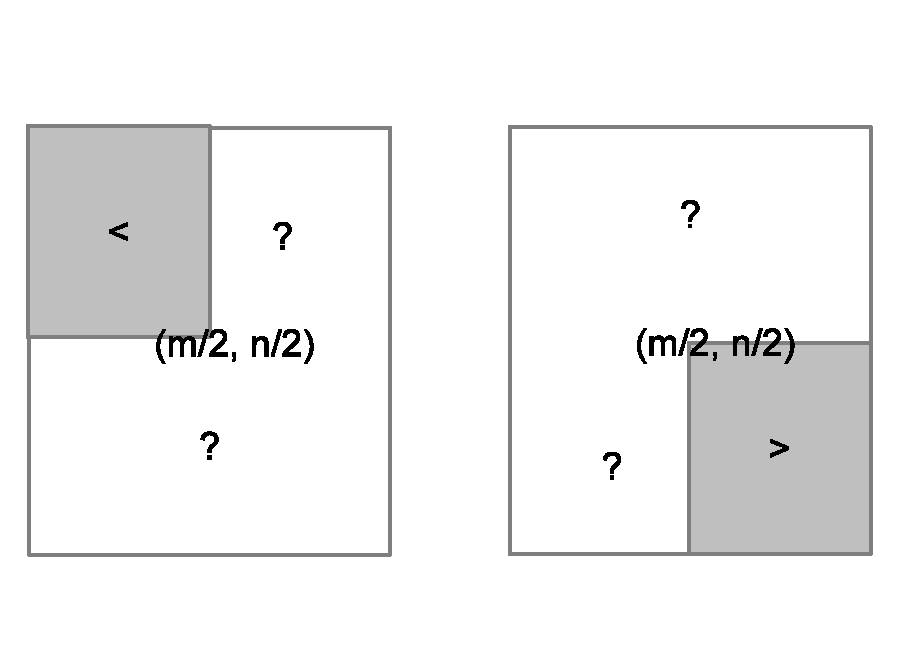
\includegraphics[scale=0.5]{img/bsearch-2D.eps}
 \caption{Left: the middle point element is smaller than $x$. All elements in the gray area are less than $x$; Right: the middle point element is greater than $x$. All elements in the gray area are greater than $x$.}
 \label{fig:bsearch-2D}
\end{figure}

The problem is that the solution domain chnages from a rectangle to a 'L' shape in both cases. We can't just
recursively apply search on it. In order to solve this problem systematically, we define the problem more
generally, use brute-force search as a start point, and keep improving it bit by bit.

Consider a function $f(x, y)$, which is strict increasing for its arguments, for instance $f(x, y) = a^x + b^y$, where
$a$ and $b$ are natural numbers. Given a value $z$, which is natural number as well. We want to sovle the equation
$f(x, y) = z$ by finding all candidate pairs $(x, y)$.

With this definition, the non-decreasing matrix search problem can be specialized by the below function.

\[
f(x, y) = \left \{
  \begin{array}
  {r@{\quad:\quad}l}
  M_{x, y} & 1 \leq x \leq m, 1 \leq y \leq n \\
  -1 & otherwise
  \end{array}
\right.
\]

\paragraph{Brute-force 2D search}

As all solutions should be found for $f(x, y)$. One can immediately give the
brute force solution by embedded looping.

\begin{algorithmic}[1]
\Function{Solve}{$f, z$}
  \State $A \gets \Phi$
  \For{$x \in \{0, 1, 2, ..., z\}$}
    \For{$y \in \{0, 1, 2, ..., z\}$}
      \If{$f(x, y) = z$}
        \State $A \gets A \cup \{(x, y)\}$
      \EndIf
    \EndFor
  \EndFor
  \State \Return $A$
\EndFunction
\end{algorithmic}

This definately calculates $f$ for $(z+1)^2$ times. It can be formalized as in (\ref{eq:bsearch-brute}).

\be
solve(f, z) = \{ (x, y) | x \in \{0, 1, ..., z\}, y \in \{0, 1, ..., z\}, f(x, y) = z\}
\label{eq:bsearch-brute}
\ee

\paragraph{Saddleback search}

We haven't utilize the fact that $f(x, y)$ is strict increasing yet. Dijkstra pointed out in \cite{saddle-back}, instead
of searching from bottom-left corner, search from the top-left leads to a effective solution. As illustrated in figure
\ref{fig:saddleback-1}, the search starts from $(0, z)$, for every point $(p, q)$, we compare $f(p, q)$ with $z$:

\begin{itemize}
\item If $f(p, q) < z$, since $f$ is strict increasing, for all $0 \leq y < q$, we have $f(p, y) < z$. We can drop all
points in the vertical line section (in red color);
\item If $f(p, q) > z$, then $f(x, q) > z$ for all $p < x \leq z$. We can drop all points in the horizontal
line section (in blue color);
\item Otherwise if $f(p, q) = z$, we mark $(p, q)$ as one solution, then both line sections can be dropped.
\end{itemize}

This is a systematical way to scale down the solution
domain rectangle. We keep dropping either a row, or a column, or both.

\begin{figure}[htbp]
 \centering
 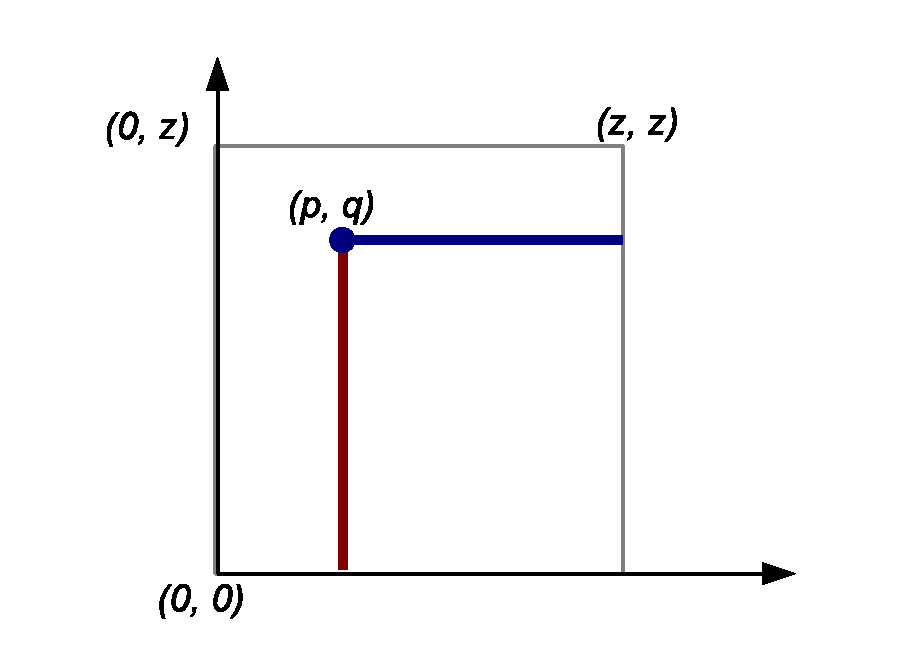
\includegraphics[scale=0.5]{img/saddleback-1.eps}
 \caption{Search from top-left.}
 \label{fig:saddleback-1}
\end{figure}

This method can be formalized as a function $search(f, z, p, q)$, which search solutions for equation $f(x, y) = z$ in
rectancle with top-left corner $(p, q)$, and bottom-right corner $(z, 0)$. We start the searching by intializing
$(p, q) = (0, z)$ as $solve(f, z) = search(f, z, 0, z)$

\be
search(f, z, p, q) =  \left \{
  \begin{array}
  {r@{\quad:\quad}l}
  \Phi & p > z \lor q < 0 \\
  search(f, z, p + 1, q) & f(p, q) < z \\
  search(f, z, p, q - 1) & f(p, q) > z \\
  \{(p, q)\} \cup search(f, z, p + 1, q - 1) & otherwise
  \end{array}
\right.
\ee

The first clause is the edge case, there is no solution if $(p, q)$ isn't on the top-left to $(z, 0)$. The following
example Haskell program implents this algorithm.

\lstset{language=Haskell}
\begin{lstlisting}
solve f z = search 0 z where
  search p q | p > z || q < 0 = []
             | z' < z = search (p + 1) q
             | z' > z = search p (q - 1)
             | otherwise = (p, q) : search (p + 1) (q - 1)
    where z' = f p q
\end{lstlisting}

Consider the calculation of $f$ is expensive, this program stores the result of $f(p, q)$ to variable $z'$.
This algorithm can also be implemented in iterative manner, that the boundaries of solution domain keeps being updated
in a loop.

\begin{algorithmic}[1]
\Function{Solve}{$f, z$}
  \State $p \gets 0, q \gets z$
  \State $S \gets \Phi$
  \While{$p \leq z \land q \geq 0$}
    \State $z' \gets f(p, q)$
    \If{$z' < z$}
      \State $p \gets p + 1$
    \ElsIf{$z' > z$}
      \State $q \gets q - 1$
    \Else
      \State $S \gets S \cup \{(p, q)\}$
      \State $p \gets p + 1, q \gets q - 1$
    \EndIf
  \EndWhile
  \State \Return $S$
\EndFunction
\end{algorithmic}

It's intuitive to translate this imperative algorithm to real program, for example, the following example Python code.

\lstset{language=Python}
\begin{lstlisting}
def solve(f, z):
    (p, q) = (0, z)
    res = []
    while p <= z and q >= 0:
        z1 = f(p, q)
        if z1 < z:
            p = p + 1
        elif z1 > z:
            q = q - 1
        else:
            res.append((p, q))
            (p, q) = (p + 1, q - 1)
    return res

\end{lstlisting}

It is clear that in every iteration, either $p$ or $q$ or both advance to the bottom-right corner by one.
Thus it takes at most $2(z+1)$ steps to complete searching. This is the worst case. There are three best
cases. The first one happens that in every iteration, both $p$ and $q$ advance by one, so that it needs
only $z+1$ steps; The second case keeps advancing horizontally to right and ends when $p$ exceeds $z$;
The last case is similar, that it keeps moving down vertically to the bottom until $q$ becomes negative.

Figure \ref{fig:saddleback-1-cases} illustrates the bese cases and the worst cases respectively. Figure
\ref{fig:saddleback-1-cases} (a) is the case that every point $(x, z-x)$ in diagonal satisfies $f(x, z-x) = z$,
it uses $z+1$ steps to arrive at $(z, 0)$; (b) is the case that every point $(x, z)$ along the top
horizontal line gives the result $f(x, z) < z$, the algorithm takes $z+1$ steps to finish; (c) is
the case that every point $(0, x)$ along the left vertical line gives the result $f(0, x) > z$, thus
the algorithm takes $z+1$ steps to finish; (d) is the worst case. If we project all the horizontal
sections along the search path to $x$ axis, the project all the vertical sections to $y$ axis, it
gives the total steps of $2(z+1)$.

\begin{figure}[htbp]
 \centering
 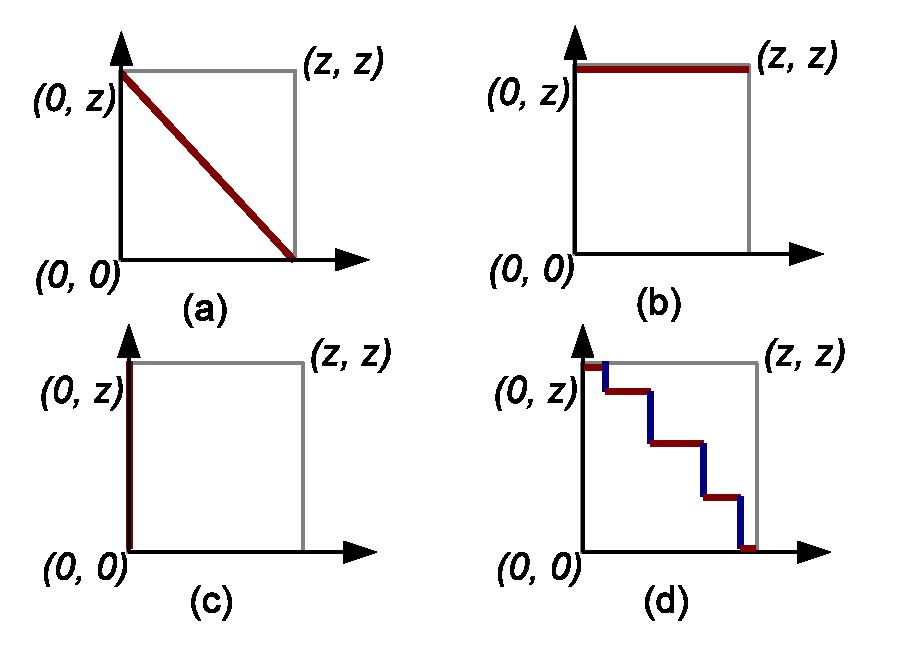
\includegraphics[scale=0.5]{img/saddleback-1-cases.eps}
 \caption{The best cases and the worst cases.}
 \label{fig:saddleback-1-cases}
\end{figure}

Compare to the quadratic brute-froce method ($O(z^2)$), we improve to a linear algorithm bound to $O(z)$.

Bird imaged that the naming `saddleback' is because the 3D plot of $f$ with the smallest bottom-left and the
latest top-right and two wings looks like a saddle as shown in figure \ref{fig:saddleback-frame}
\begin{figure}[htbp]
 \centering
 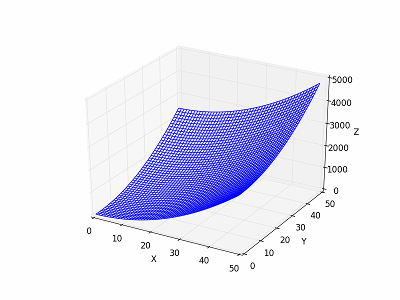
\includegraphics[scale=0.8]{img/saddleback-xx-yy.eps}
 \caption{Plot of $f(x, y) = x^2 + y^2$.}
 \label{fig:saddleback-frame}
\end{figure}

\paragraph{Improved saddleback search}

We haven't utilized the binary search tool so far, even the problem extends to 2-dimension domain.
The basic saddleback search starts from the top-left corner $(0, z)$ to the bottom-right corner $(z, 0)$.
This is acutally over-general domain. we can constrait it a bit more accurate.

Since $f$ is strict increasing, we can find the biggest number $m$, that $0 \leq m \leq z$, along the
$y$ axis which satisfies $f(0, m) \leq z$; Similarly, we can find the biggest $n$, that $0 \leq n \leq z$,
along the $x$ axis, which satisifes $f(n, 0) \leq z$; And the solution domain shrinks
from $(0, z) - (z, 0)$ to $(0, m) - (n, 0)$ as shown in figure \ref{fig:saddleback-2}.

\begin{figure}[htbp]
 \centering
 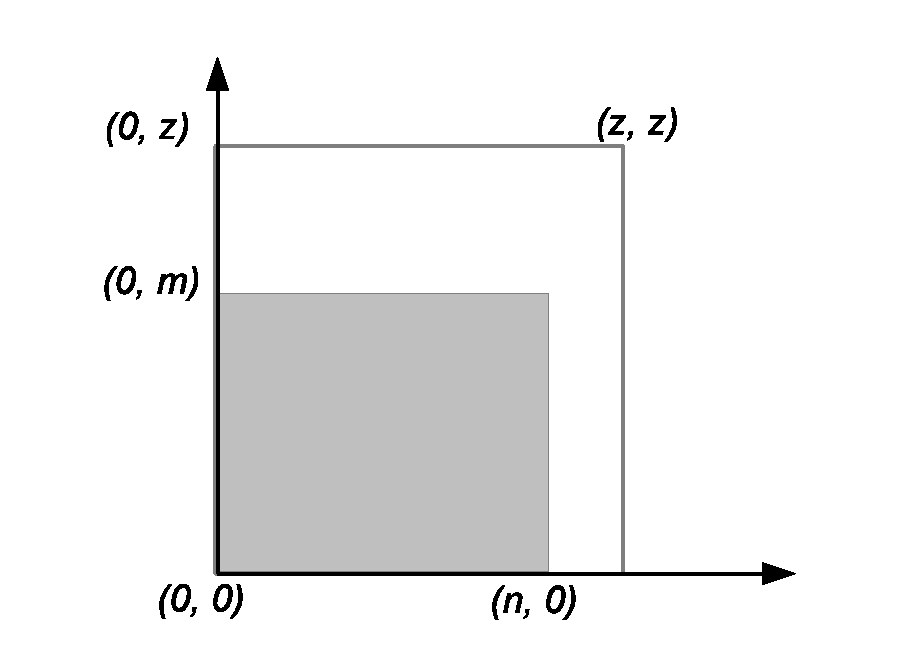
\includegraphics[scale=0.5]{img/saddleback-2.eps}
 \caption{A more accurate search domain shown in shaded color.}
 \label{fig:saddleback-2}
\end{figure}

Of course $m$ and $n$ can be found by brute-force searching like below.

\be
\begin{array}{rl}
m & = max(\{y | 0 \leq y \leq z, f(0, y) \leq z\}) \\
n & = max(\{x | 0 \leq x \leq z, f(x, 0) \leq z\})
\end{array}
\ee

When searching $m$, the $x$ variable of $f$ is bound to 0. It turns to be one dimension search problem
for a strict increasing function (or in functional term, a Curried function $f(0, y)$). Binary search works
in such case. However, we need a bit modification for equation (\ref{eq:bsearch}). Different from searching
a solution $l \leq x \leq u$, so that $f(x) = y$ for a given $y$; we need search for a solution
$l \leq x \leq u$ so that $f(x) \leq y < f(x+1)$.

\be
bsearch(f, y, l, u) = \left \{
  \begin{array}
  {r@{\quad:\quad}l}
  l & u \leq l \\
  m & f(m) \leq y < f(m+1), m = \lfloor \frac{l + u}{2} \rfloor \\
  bsearch(f, y, m + 1, u) & f(m) \leq y \\
  bsearch(f, y, l, m-1) & otherwise
  \end{array}
\right.
\label{eq:bsearch-general}
\ee

The first clause handles the edge case that the range contains less than one integer. The lower
boundary is returned in such case;
If the middle point produces a value less than or equal to the target, while the next one evaluates
to a bigger value, the middle point is what we are looking for;
Otherwise if the point next to the middle also evaluates to a value not greater than the target,
the lower bound is increased by one, and we perform recursively binary search;
The only left case is that, the middle point evaluates to a value greater than the target,
upperbound is updated as the point preceeds to the middle for furthur recursive searching. The following
Haskell example code implements this modified binary search.

\lstset{language=Haskell}
\begin{lstlisting}
bsearch f y (l, u) | u <= l = l
                   | f m <= y = if f (m + 1) <= y then bsearch f y (m + 1, u) else m
                   | otherwise = bsearch f y (l, m-1)
  where m = (l + u) `div` 2
\end{lstlisting}

Then $m$ and $n$ can be found by using this binary search function.

\be
\begin{array}{rl}
m & = bsearch(\lambda_y \cdot f(0, y), z, 0, z) \\
n & = bsearch(\lambda_x \cdot f(x, 0), z, 0, z)
\end{array}
\label{eq:bsearch-boundaries}
\ee

And the improved saddleback search shrinks to this new search domain $solve(f, z) = search(f, z, 0, m)$:

\be
search(f, z, p, q) =  \left \{
  \begin{array}
  {r@{\quad:\quad}l}
  \Phi & p > n \lor q < 0 \\
  search(f, z, p + 1, q) & f(p, q) < z \\
  search(f, z, p, q - 1) & f(p, q) > z \\
  \{(p, q)\} \cup search(f, z, p + 1, q - 1) & otherwise
  \end{array}
\right.
\ee

It's almost as same as the basic saddleback version, except that it stops if $p$ exceeds $n$, but not $z$.
In real implementation, the result of $f(p, q)$ can be calculated once, and stored in a variable as
shown in the following Haskell example.

\lstset{language=Haskell}
\begin{lstlisting}
solve' f z = search 0 m where
  search p q | p > n || q < 0 = []
             | z' < z = search (p + 1) q
             | z' > z = search p (q - 1)
             | otherwise = (p, q) : search (p + 1) (q - 1)
    where z' = f p q
  m = bsearch (f 0) z (0, z)
  n = bsearch (\x->f x 0) z (0, z)
\end{lstlisting}

This improved saddleback firstly performs binary search two rounds to find the proper $m$, and $n$.
Eash round is bound to $O(\lg z)$ times of calculation for $f$; After that, it takes $O(m + n)$
time in the worst case; and $O(min(m, n))$ time in the best case. The overall performance is
given in the following table.

\begin{tabular}{|l|l|}
\hline
 & times of evaluation $f$ \\
\hline
worst case & $2 \log z + m + n$ \\
best case & $2 \log z + min(m, n)$ \\
\hline
\end{tabular}

For some function $f(x, y) = a^x + b^y$, for positive integers $a$ and $b$, $m$ and $n$ will be
relative small, that the performance is near to $O(\lg z)$.

This algorithm can also be realized in imperative approach. Firstly, the binary search should be modified.

\begin{algorithmic}[1]
\Function{Binary-Search}{$f, y, (l, u)$}
  \While{$l < u$}
    \State $m \gets \lfloor \frac{l + u}{2} \rfloor$
    \If{$f(m) \leq y$}
      \If{$y < f(m+1)$}
        \State \Return m
      \EndIf
      \State $l \gets m + 1$
    \Else
      \State $u \gets m$
    \EndIf
  \EndWhile
  \State \Return $l$
\EndFunction
\end{algorithmic}

Utilize this algorithm, the boundaries $m$ and $n$ can be found before performing the saddleback search.

\begin{algorithmic}[1]
\Function{Solve}{$f, z$}
  \State $m \gets$ \Call{Binary-Search}{$\lambda_y \cdot f(0, y), z, (0, z)$}
  \State $n \gets$ \Call{Binary-Search}{$\lambda_x \cdot f(x, 0), z, (0, z)$}
  \State $p \gets 0, q \gets m$
  \State $S \gets \Phi$
  \While{$p \leq n \land q \geq 0$}
    \State $z' \gets f(p, q)$
    \If{$z' < z$}
      \State $p \gets p + 1$
    \ElsIf{$z' > z$}
      \State $q \gets q - 1$
    \Else
      \State $S \gets S \cup \{(p, q)\}$
      \State $p \gets p + 1, q \gets q - 1$
    \EndIf
  \EndWhile
  \State \Return $S$
\EndFunction
\end{algorithmic}

The implementation is left as exercise to the reader.

\paragraph{More improvement to saddleback search}

In figure \ref{fig:bsearch-2D}, two cases are shown for comparing the value of the middle point in a matirx with the given value.
One case is the center value is smaller than the given value, the other is bigger. In both case, we can only throw away
$\frac{1}{4}$ candidates, and left a 'L' shape for further searching.

Actually, one important case is missing. We can extend the observation to any point inside the rectagle searching area.
As shown in the figure \ref{fig:saddleback-drop}.

\begin{figure}[htbp]
 \centering
 \subfloat[If $f(p, q) \neq z$, only lower-left or upper-right sub area (in gray color) can be thrown. Both left a 'L' shape.]{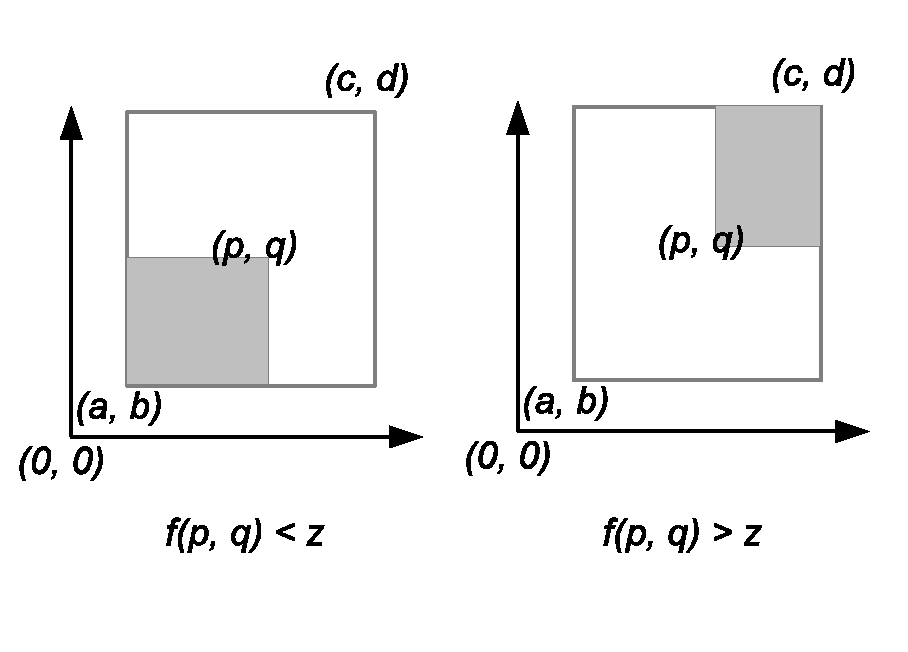
\includegraphics[scale=0.5]{img/saddleback-3.eps}} \\
 \subfloat[If $f(p, q) = z$, both sub areas can be thrown, the scale of the problem is halved.]{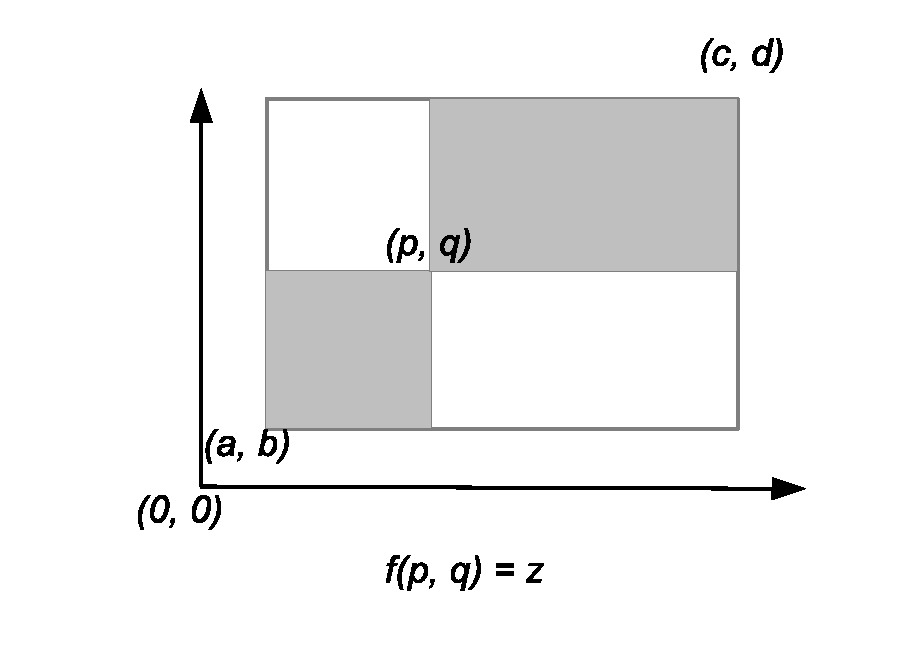
\includegraphics[scale=0.5]{img/saddleback-4.eps}}
 \caption{The efficiency of scaling down the search domain.}
 \label{fig:saddleback-drop}
\end{figure}

Suppose we are searching in a rectangle from the lower-left corner $(a, b)$ to the upper-right corner $(c, d)$.
If the $(p, q)$ isn't the middle point, and $f(p, q) \neq z$. We can't ensure the area to be dropped is always
1/4. However, if $f(p, q) = z$, as $f$ is strict increasing, we are not only sure both the lower-left and the
upper-right sub areas can be thrown, but also all the other points in the column $p$ and row $q$. The problem
can be scaled down fast, because only 1/2 area is left.

This indicates us, instead of jumping to the middle point to start searching. A more efficient way is to find
a point which evaluates to the target value. One straightforward way to find such a point, is to perform
binary search along the center horizontal line or the center vertical line of the rectangle.

The performance of binary search along a line is the length of that line. A good idea is alway pick the shorter
center line as shown in figure \ref{fig:saddleback-centerline}. That if the height of the rectangle is longer
than the width, we perform binary search along the horizontal center line; otherwise we choose the vertical
center line.

\begin{figure}[htbp]
 \centering
 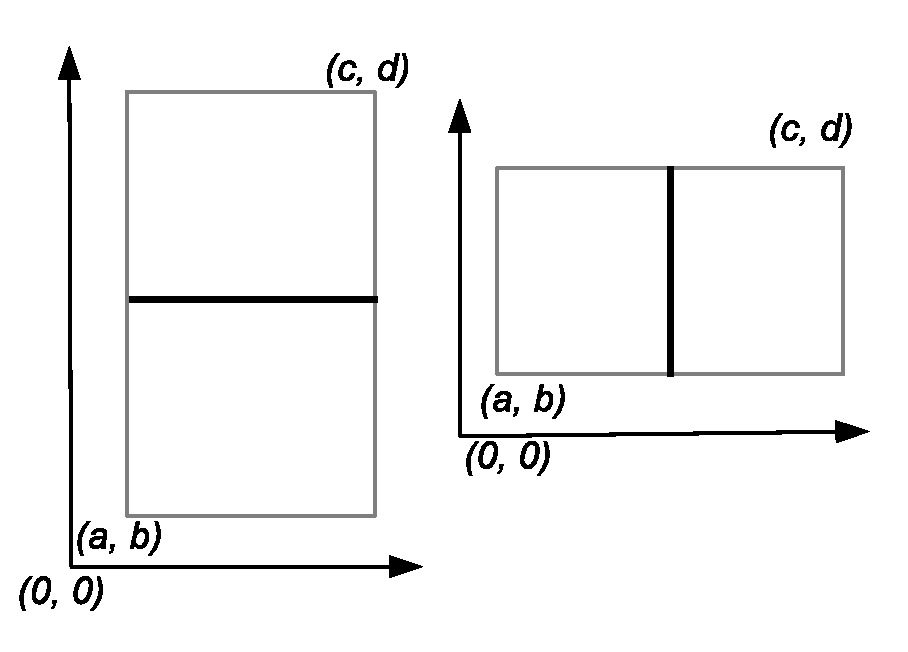
\includegraphics[scale=0.5]{img/saddleback-centerline.eps}
 \caption{Binary search along the shorter center line.}
 \label{fig:saddleback-centerline}
\end{figure}

However, what if we can't find a point $(p, q)$ in the center line, that satisfies $f(p, q) = z$? Let's take
the center horizontal line for example. even in such case, we can still search for a point that
$f(p, q) < z < f(p+1, q)$. The only difference is that we can't drop the points in row $p$ and $q$ completely.

Combine this condition, the binary search along the horinzontal line is to find a $p$, satisifies
$f(p, q) \leq z < f(p+1, q)$; While the vertical line search condition is $f(p, q) \leq z < f(p, q + 1)$.

The modified binary serach ensures that, if all points in the line segment give $f(p, q) < z$, the upper
bound will be found; and the lower bound will be found if they all greater than $z$. We can drop the
whole area on one side of the center line in such case.

Sum up all the ideas, we can develop a effcient improved saddleback search as the following.

\begin{enumerate}
\item Perform binary search along the $y$ axis and $x$ axis to find the tight boundaries from $(0, m)$ to $(n, 0)$;
\item Denote the candidate rectangle as $(a, b) - (c, d)$, if the candidate rectangle is empty, the solution is empty;
\item If the height of the rectangle is longer than the width, perform binary search along the center horinzontal line; otherwise, perform binary search along the center vertical line; denote the search result as $(p, q)$;
\item If $f(p, q) = z$, record $(p, q)$ as a solution, and recursively search two sub rectangles $(a, b) - (p-1, q+1)$ and
$(p+1, q-1) - (c, d)$;
\item Otherwise, $f(p, q) \neq z$, recursively the same two sub rectangles plus a line section. The line section
is either $(p, q+1) - (p, b)$ as shown in figure \ref{fig:include-line} (a); or $(p+1, q) - (c, q)$ as shown in
figure \ref{fig:include-line} (b).
\end{enumerate}

\begin{figure}[htbp]
 \centering
 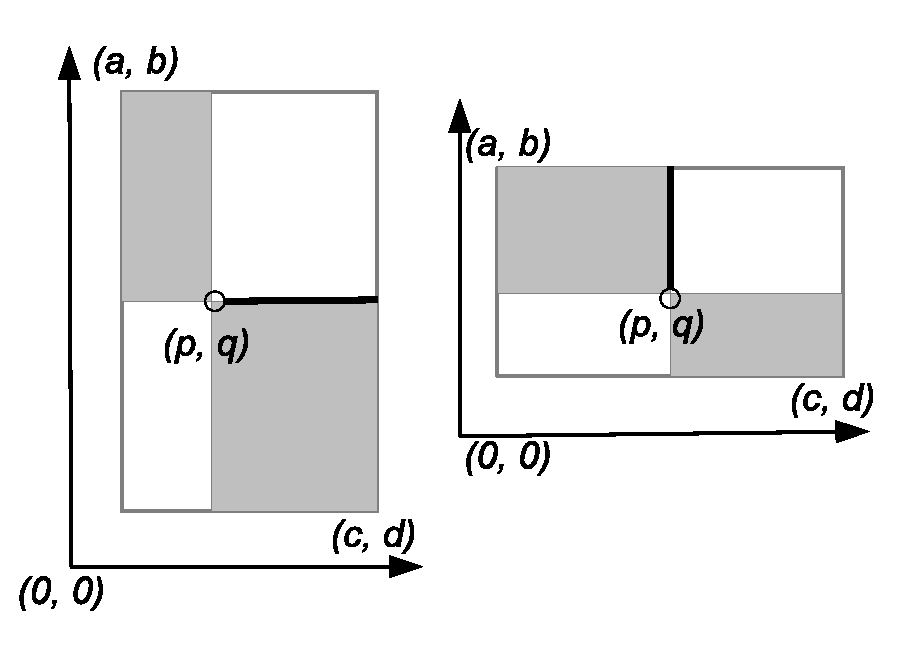
\includegraphics[scale=0.5]{img/saddleback-include-ln.eps}
 \caption{Recursively search the gray areas, the bold line should be included if $f(p, q) \neq z$.}
 \label{fig:include-line}
\end{figure}

This algorithm can be formalized as the following. The equation (\ref{eq:bsearch-general}), and (\ref{eq:bsearch-boundaries})
are as same as before. A new $search$ function should be defined.

Define $Search_{(a, b), (c, d)}$ as a function for searching rectangle with top-left corner $(a, b)$,
and bottom-right corner $(c, d)$.

\be
search_{(a, b), (c, d)} =  \left \{
  \begin{array}
  {r@{\quad:\quad}l}
  \Phi & c < a \lor d < b \\
  csearch & c - a < b - d \\
  rsearch & otherwise
  \end{array}
\right.
\ee

Function $csearch$ perfroms binary search in the center horinzontal line to find a point $(p, q)$ that
$f(p, q) \leq z < f(p+1, q)$. This is shown in figure \ref{fig:include-line} (a).
There is a special edge case, that all points in the lines evaluate to values greater than $z$. The general binary search
will return the lower bound as result, so that $(p, q) = (a, \lfloor \frac{b + d}{2} \rfloor)$. The whole upper side
includes the center line can be dropped as shown in figure \ref{fig:saddleback-edge-cases} (a).

\begin{figure}[htbp]
 \centering
 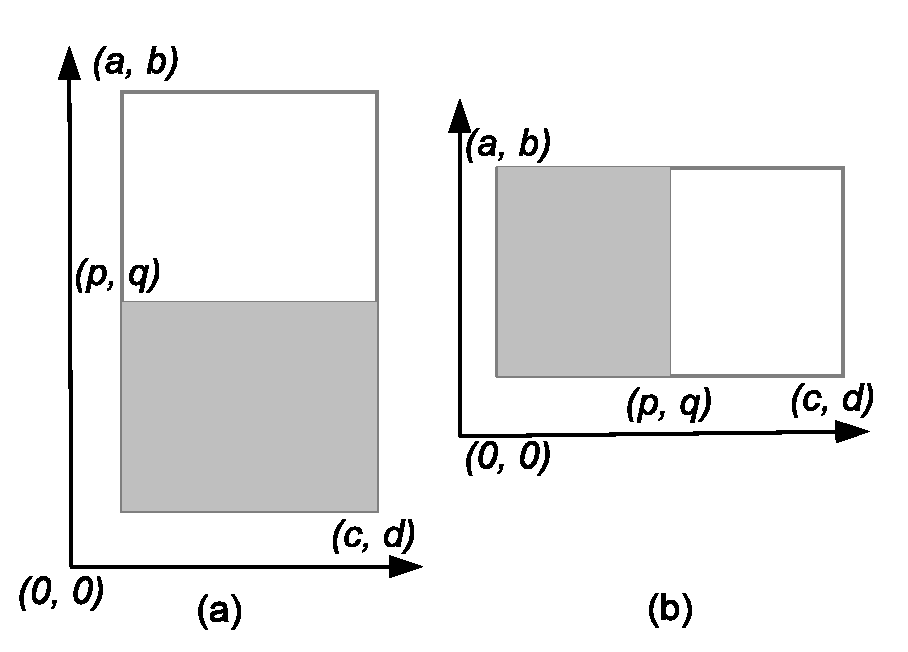
\includegraphics[scale=0.5]{img/saddleback-edge-cases.eps}
 \caption{Edge cases when performing binary search in the center line.}
 \label{fig:saddleback-edge-cases}
\end{figure}

\be
csearch = \left \{
  \begin{array}
  {r@{\quad:\quad}l}
  search_{(p, q-1), (c, d)} & z < f(p, q) \\
  search_{(a, b), (p-1, q+1)} \cup \{(p, q)\} \cup search_{(p+1, q-1), (c, d)} & f(p, q) = z \\
  search_{(a, b), (p, q+1)} \cup search_{(p+1, q-1), (c, d)} & otherwise
  \end{array}
\right.
\ee

Where

\[
\begin{array}{l}
q = \lfloor \frac{b + d}{2} \rfloor) \\
p = bsearch(\lambda_x \cdot f(x, q), z, (a, c))
\end{array}
\]

Function $rsearch$ is quite similar except that it searches in the center horinzental line.

\be
rsearch = \left \{
  \begin{array}
  {r@{\quad:\quad}l}
  search_{(a, b), (p - 1, q)} & z < f(p, q) \\
  search_{(a, b), (p-1, q+1)} \cup \{(p, q)\} \cup search_{(p+1, q-1), (c, d)} & f(p, q) = z \\
  search_{(a, b), (p-1, q+1)} \cup search_{(p+1, q), (c, d)} & otherwise
  \end{array}
\right.
\ee

Where

\[
\begin{array}{l}
p = \lfloor \frac{a + c}{2} \rfloor) \\
q = bsearch(\lambda_y \cdot f(p, y), z, (d, b))
\end{array}
\]

The following Haskell program implements this algorithm.

\lstset{language=Haskell}
\begin{lstlisting}
search f z (a, b) (c, d) | c < a || b < d = []
                         | c - a < b - d = let q = (b + d) `div` 2 in
                                             csearch (bsearch (\x -> f x q) z (a, c), q)
                         | otherwise = let p = (a + c) `div` 2 in
                                             rsearch (p, bsearch (f p) z (d, b))
  where
    csearch (p, q) | z < f p q = search f z (p, q - 1) (c, d)
                   | f p q == z = search f z (a, b) (p - 1, q + 1) ++
                                    (p, q) : search f z (p + 1, q - 1) (c, d)
                   | otherwise = search f z (a, b) (p, q + 1) ++
                                   search f z (p + 1, q - 1) (c, d)
    rsearch (p, q) | z < f p q = search f z (a, b) (p - 1, q)
                   | f p q == z = search f z (a, b) (p - 1, q + 1) ++
                                    (p, q) : search f z (p + 1, q - 1) (c, d)
                   | otherwise = search f z (a, b) (p - 1, q + 1) ++
                                    search f z (p + 1, q) (c, d)
\end{lstlisting}

And the main program calls this function after performing binary search in $X$ and $Y$ axes.

\lstset{language=Haskell}
\begin{lstlisting}
solve f z = search f z (0, m) (n, 0) where
  m = bsearch (f 0) z (0, z)
  n = bsearch (\x -> f x 0) z (0, z)
\end{lstlisting}

Since we drop half areas in every recursion, it takes $O(\log (mn))$ rounds of search. However, in order to
locate the point $(p, q)$, which halves the problem, we must perform binary search along the center line.
which will call $f$ about $O(\log(min(m, n)))$ times. Denote the time of searching a $m \times n$ rectangle
as $T(m, n)$, the recursion relation ship can be represented as the following.

\be
T(m, n) = \log(min(m, n)) + 2 T(\frac{m}{2}, \frac{n}{2})
\ee

Suppose $m > n$, using telescope method, for $m = 2^i$, and $n = 2^j$. We have:

\be
\begin{array}{rl}
T(2^i, 2^j) & = j + 2 T(2^{i-1}, 2^{j-1}) \\
            & = \displaystyle \sum_{k=0}^{i-1} 2^k(j - k) \\
            & = O(2^i(j-i)) \\
            & = O(m \log (n/m))
\end{array}
\ee

Richard Bird proved that this is asymptotically optimal by a lower bound of searching a given value in
$m \times n$ rectangle \cite{fp-pearls}.

The imperative algorithm is almost as same as the funcitonal version. We skip it for the sake of brevity.

\begin{Exercise}
\begin{itemize}
\item Prove that the average case of the divide and conquer solution to $k$-selection problem is $O(n)$. Please refer to previous chapter about quick sort.
\item Implement the imperative $k$-selection problem with 2-way partition, and median-of-three pivot selection.
\item Implement the imperative $k$-selection problem to handle duplicated elements effectively.
\item Realize the median-of-median $k$-selection algorithm and implement it in your favorite programming language.
\item The $tops(k, L)$ algorithm uses list concatenation likes $A \cup \{ l_1 \} \cup tops(k - |A| - 1, B)$. It is linear operation which is proportion to the length of the list to be concatenated. Modify the algorithm so that the sub lists are concatenated by one pass.
\item The author considered another divide and conquer solution for the $k$-selection problem. It finds the maximum of the
first $k$ elements and the minimum of the rest. Denote them as $x$, and $y$. If $x$ is smaller than $y$, it means that
all the first $k$ elements are smaller than the rest, so that they are exactly the top $k$ smallest; Otherwise, There
some elements in the first $k$ should be moved.
\begin{algorithmic}[1]
\Procedure{Tops}{$k, A$}
  \State $l \gets 1$
  \State $u \gets |A|$
  \Loop
    \State $i \gets$ \Call{Max-At}{$A[l..k]$}
    \State $j \gets$ \Call{Min-At}{$A[k+1..u]$}
    \If{$A[i] < A[j]$}
      \State break
    \EndIf
    \State \textproc{Exchange} $A[l] \leftrightarrow A[j]$
    \State \textproc{Exchange} $A[k+1] \leftrightarrow A[i]$
    \State $l \gets$ \Call{Partition}{$A, l, k$}
    \State $u \gets$ \Call{Partition}{$A, k+1, u$}
  \EndLoop
\EndProcedure
\end{algorithmic}
Explain why this algorithm works? What's the performance of it?
\item Implement the binary search algorithm in both recursive and iterative manner, and try to verify your version
automatically. You can generate randomized data, test your program with the binary search invariant and against the
one provided in your standard library.
\item Implement the improved saddleback search by first performing binary search to find a more accurate solution domain
in your favorite imperative programming language.
\item Realize the improved 2D search, by performing binary search along the shorter center line, in your favorite
imprative programming language.
\item Someone considers that the 2D search can be designed as the following. When search a rectangle, as the
minimum value is at bottom-left, and the maximum at to-right. If the target value is less than the minimum or
greater than the maximum, then there is no solution; otherwise, the rectangle is divided into 4 sub renctangles
at the center point, then perform recursively searching.
\begin{algorithmic}[1]
\Procedure{Search}{$f, z, a, b, c, d$} \Comment{$(a, b)$: bottom-left $(c, d)$: top-right}
  \If {$z \leq f(a, b) \lor f(c, d) \geq z$}
    \If{$z = f(a, b)$}
      \State record $(a, b)$ as a solution
    \EndIf
    \If{$z = f(c, d)$}
      \State record $(c, d)$ as a solution
    \EndIf
    \State \Return
  \EndIf
  \State $p \gets \lfloor \frac{a + c}{2} \rfloor$
  \State $q \gets \lfloor \frac{b + d}{2} \rfloor$
  \State \Call{Search}{$f, z, a, q, p, d$}
  \State \Call{Search}{$f, z, p, q, c, d$}
  \State \Call{Search}{$f, z, a, b, p, q$}
  \State \Call{Search}{$f, z, p, b, c, q$}
\EndProcedure
\end{algorithmic}
What's the performance of this algorithm?
\end{itemize}
\end{Exercise}

\subsection{Information reuse}
One interesting behavior that human search things is that people learn while searching. We do not only
remember lessons which cause search fails, but also learn patterns which lead to success. This is a
kind of information reusing, no matter the infomation is positive or negative. However, It's not easy
to determine what information should be kept for further searching. Too little infomration isn't
enough to help effective searching, while keeping too much is expensive in term of spaces.

In this section, we'll first introduce two interesting problems, Boyer-Moore majority number problem
and the maximum sum of sub vector problem. Both resuses information as little as possible. Next two
popular string matching algorithm, Knuth-Morris-Pratt algorithm and Boyer-Moore algorithm will be
introduced.

\subsubsection{Boyer-Moore majority number}

Voting is quite ciritical to people. We use voting to select the leader, to make decision or reject a
proposal. In the months when I was writing this chapter, there are three countries in the world voted their
presidents. All of the three voting acitivites utilized computer to calculate the result.

Suppose there is a country in a small island wants to select a new president. According to the constitution
of this country, only if the candidate win more than half of the voting can be selected as the
president. Given a serious of votes, such as A, B, A, C, B, B, D, ...,
can we develop a program tells who is the new president if there is,
or indicate nobody wins more than half of the votes?

Of course this problem can be solved with brute-force by uisng a map. As what we did in the chapter
of binary search tree.

\lstset{language=C++}
\begin{lstlisting}
template<typename T>
T majority(const T* xs, int n, T fail) {
    map<T, int> m;
    int i, max = 0;
    T r;
    for (i = 0; i < n; ++i)
        ++m[xs[i]];
    for (typename map<T, int>::iterator it = m.begin(); it != m.end(); ++it)
        if (it->second > max) {
            max = it->second;
            r = it->first;
        }
    return max * 2 > n ? r : fail;
}
\end{lstlisting}

This program first scan the votes, and accumulates the number of votes for each individual with a map.
After that, it traverse the map to find the one with most of votes. If the number of votes is bigger
than half of the total, the element is output otherwise, it returns a value to indicate fail.

The following pseudo code decribes this algorithm.

\begin{algorithmic}[1]
\Function{Majority}{$A$}
  \State $M \gets $ empty map
  \For{$\forall a \in A$}
    \State \textproc{Put}($M$, $a, 1 + $ \Call{Get}{$M, a$})
  \EndFor
  \State $max \gets 0$, $m \gets NIL$
  \For{$\forall (k, v) \in M$}
    \If{$max < v$}
      \State $max \gets v$, $m \gets k$
    \EndIf
  \EndFor
  \If{$max > |A| 50\%$}
    \State \Return $m$
  \Else
    \State fail
  \EndIf
\EndFunction
\end{algorithmic}

For $m$ individuals and $n$ votes, this program firstly takes about $O(n \log m)$ to build the map if
the map is implemented in self balanced tree (red-black tree for instance); or about $O(n)$ time if
the map is implemented in hash table. However, the hash table needs more space. Next the program
takes $O(m)$ time to traverse the map, and find the majority vote. The following table lists the
time and space performance for different maps.

\begin{tabular}{|l|l|l|}
\hline
map & time & space \\
\hline
self-balanced tree & $O(n \log m)$ & $O(m)$ \\
hashing & $O(n)$ & $O(m)$ at least \\
\hline
\end{tabular}

Boyer and Moore invented a cleaver algorithm in 1980, which can pick the majority element with only
one scan if there is. Their algorithm only needs $O(1)$ space \cite{boyer-moore-majority}.

The idea is that, record the first candidate as the winner so far, and mark he wins 1 vote. During
the scan process, if the winner being selected gets another vote, we just increase the vote counter;
otherwise, it means somebody vote against this candidate, so the vote counter should be decreased
by one. If the vote counter becomes zero, it means this candidate is voted out; We select
the next candidate as the new winner and repeate the above scanning process.

Suppose there is a series of votes: A, B, C, B, B, C, A, B, A, B, B, D, B.
Below table illustrates the steps of this processing.

\begin{tabular}{|l|l|l|}
\hline
winer & count & scan position \\
\hline
A & 1 & {\bf A}, B, C, B, B, C, A, B, A, B, B, D, B \\
A & 0 & A, {\bf B}, C, B, B, C, A, B, A, B, B, D, B \\
C & 1 & A, B, {\bf C}, B, B, C, A, B, A, B, B, D, B \\
C & 0 & A, B, C, {\bf B}, B, C, A, B, A, B, B, D, B \\
B & 1 & A, B, C, B, {\bf B}, C, A, B, A, B, B, D, B \\
B & 0 & A, B, C, B, B, {\bf C}, A, B, A, B, B, D, B \\
A & 1 & A, B, C, B, B, C, {\bf A}, B, A, B, B, D, B \\
A & 0 & A, B, C, B, B, C, A, {\bf B}, A, B, B, D, B \\
A & 1 & A, B, C, B, B, C, A, B, {\bf A}, B, B, D, B \\
A & 0 & A, B, C, B, B, C, A, B, A, {\bf B}, B, D, B \\
B & 1 & A, B, C, B, B, C, A, B, A, B, {\bf B}, D, B \\
B & 0 & A, B, C, B, B, C, A, B, A, B, B, {\bf D}, B \\
B & 1 & A, B, C, B, B, C, A, B, A, B, B, D, {\bf B} \\
\hline
\end{tabular}

The key point is that, if there exits majority greater than 50\%, it can't be voted out
by all the others. However, if there are not any candidates win more than half of the votes, the recorded
`winner' is invalid. Thus it is neccessary to perform a second round scan for verification.

The following pseudo code illustrates this algorithm.

\begin{algorithmic}[1]
\Function{Majority}{$A$}
  \State $c \gets 0$
  \For{$i \gets$ 1 to $|A|$}
    \If{$c = 0$}
      \State $x \gets A[i]$
    \EndIf
    \If{$A[i] = x$}
      \State $c \gets c + 1$
    \Else
      \State $c \gets c - 1$
    \EndIf
  \EndFor
  \State \Return $x$
\EndFunction
\end{algorithmic}

If there is the majority element, this algorithm takes one pass to scan the votes. In every
iteration, it either increases or decreases the counter according to the vote is support
or against the current selection. If the counter becomes zero, it means the current
selection is voted out. So the new one is selected as the updated candiate for further scan.

The process is linear $O(n)$ time, and the spaces needed are just two variables. One
for recording the selected candidate so far, the other is for vote counting.

Athough this algorithm can find the majority element if there is. it still picks an element
even there isn't. It is neccessary to scan the votes for the second round for verification.

\begin{algorithmic}[1]
\Function{Majority}{$A$}
  \State $c \gets 0$
  \For{$i \gets$ 1 to $|A|$}
    \If{$c = 0$}
      \State $x \gets A[i]$
    \EndIf
    \If{$A[i] = x$}
      \State $c \gets c + 1$
    \Else
      \State $c \gets c - 1$
    \EndIf
  \EndFor
  \State $c \gets 0$
  \For{$i \gets 1$ to $|A|$}
    \If{$A[i] = x$}
      \State $c \gets c + 1$
    \EndIf
  \EndFor
  \If{$c > \%50|A|$}
    \State \Return $x$
  \Else
    \State fail
  \EndIf
\EndFunction
\end{algorithmic}

Even with this verification process, the algorithm is still bound to $O(n)$ time, and the
space needed is constant. The following ISO C++ program implements this algorithm \footnote{We acutally
uses the ANSI C style. Only C++ template is used to generalize the type of the element}.

\lstset{language=C++}
\begin{lstlisting}
template<typename T>
T majority(const T* xs, int n, T fail) {
    T m;
    int i, c;
    for (i = 0, c = 0; i < n; ++i) {
        if (!c)
            m = xs[i];
        c += xs[i] == m ? 1 : -1;
    }
    for (i = 0, c = 0; i < n; ++i, c += xs[i] == m);
    return c * 2 > n ? m : fail;
}
\end{lstlisting}

Boyer-Moore majority algorithm can also be realized in pure functional approach. Different from the
imperative settings, which use variables to record and update infomation, accumulators are
used to define the core algorithm. Define function $maj(c, n, L)$, which takes a list of votes $L$,
a selected candidate $c$ so far, and a counter $n$. For non empty list $L$, we initialize $c$ as
the first vote $l_1$, and set the counter as 1 to start the algorithm: $maj(l_1, 1, L')$, where
$L'$ is the rest votes except for $l_1$. Below are the definition of this funciton.

\be
maj(c, n, L) = \left \{
  \begin{array}
  {r@{\quad:\quad}l}
  c & L = \Phi \\
  maj(c, n + 1, L') & l_1 = c \\
  maj(l_1, 1, L') & n = 0 \land l_1 \neq c \\
  maj(c, n - 1, L') & otherwise
  \end{array}
\right.
\ee

We also need to define a function, which can verify the result. The idea is that, if the list of votes
is empty, the final result is a failure; otherwise, we start the Boyer-moore algorithm to find a
candiate $c$, then we count the list again to get the total votes $c$ wins, and verify if $c$ wins
at least half votes.

\be
majority(L) = \left \{
  \begin{array}
  {r@{\quad:\quad}l}
  fail & L = \Phi \\
  c & c = maj(l_1, 1, L'), |\{x | x \in L, x = c\}| > \%50 |L| \\
  fail & otherwise
  \end{array}
\right.
\ee

Below Haskell example code implements this algorithm.

\lstset{language=Haskell}
\begin{lstlisting}
majority :: (Eq a) => [a] -> Maybe a
majority [] = Nothing
majority (x:xs) = let m = maj x 1 xs in verify m (x:xs)

maj c n [] = c
maj c n (x:xs) | c == x = maj c (n+1) xs
               | n == 0 = maj x 1 xs
               | otherwise = maj c (n-1) xs

verify m xs = if 2 * (length $ filter (==m) xs) > length xs then Just m else Nothing
\end{lstlisting} %$

\subsubsection{Maximum sum of sub vector}
Jon Bentley presents another interesting puzzle which can be solved by using quite similar idea in \cite{programming-pearls}.
The problem is to find the maximum sum of sub vector. For example in the following array, The sub vector
\{19, -12, 1, 9, 18\} yields the biggest sum 35.

\begin{tabular}{|c|c|c|c|c|c|c|c|c|c|}
\hline
3 & -13 & 19 & -12 & 1 & 9 & 18 & -16 & 15 & -15 \\
\hline
\end{tabular}

Note that it is only required to ouput the value of the maximum sum. If all the numbers are positive, the answer is
definitely the sum of all. Another special case is that all numbers are negative. We define the maximum sum is 0 for
an empty sub vector.

Of course we can find the anwser by brute-force calculating all sums of sub vectors and pick the maximum. Such naive
method is typical quadratic.

\begin{algorithmic}[1]
\Function{Max-Sum}{$A$}
  \State $m \gets 0$
  \For{$i \gets 1$ to $|A|$}
    \State $s \gets 0$
    \For{$j \gets i$ to $|A|$}
      \State $s \gets s + A[j]$
      \State $m \gets $ \Call{Max}{$m, s$}
    \EndFor
  \EndFor
  \State \Return $m$
\EndFunction
\end{algorithmic}

The brute force algorithm does not reuse any information in previous search. Similar with Boyer-Moore majority
vote algorithm, we can record the maximum sum end to the position where we are scaning. Of course we also need
record the biggest sum found so far. The following figure illustrates this idea and the invariant during scan.

\begin{figure}[htbp]
 \centering
 \includegraphics[scale=0.5]{img/max-sum-invariant.ps}
 \caption{Invariant during scan.}
 \label{fig:max-sum-invariant}
\end{figure}

At any time when we scan to the $i$-th position, the max sum found so far is recorded as $A$. At the same time, we
also record the biggest sum end at $i$ as $B$. Note that $A$ and $B$ may not be the same, infact, we always maintain
$B \leq A$. and when $B$ becomes greater than $A$ by adding with the next element,
we update $A$ with this new value. When $B$ becomes negative, this happens when the next element is a negative number,
we reset it to 0. The following tables illustrated the steps when we scan the example vector
$\{3, -13, 19, -12, 1, 9, 18, -16, 15, -15\}$.

\begin{tabular}{|l|l|r|}
\hline
max sum & max end at $i$ & list to be scan \\
\hline
0 & 0 & $\{3, -13, 19, -12, 1, 9, 18, -16, 15, -15\}$ \\
3 & 3 & $\{-13, 19, -12, 1, 9, 18, -16, 15, -15\}$ \\
3 & 0 & $\{19, -12, 1, 9, 18, -16, 15, -15\}$ \\
22 & 19 & $\{-12, 1, 9, 18, -16, 15, -15\}$ \\
22 & 7 & $\{1, 9, 18, -16, 15, -15\}$ \\
22 & 8 & $\{9, 18, -16, 15, -15\}$ \\
22 & 17 & $\{18, -16, 15, -15\}$ \\
35 & 35 & $\{-16, 15, -15\}$ \\
35 & 19 & $\{15, -15\}$ \\
35 & 34 & $\{-15\}$ \\
35 & 19 & $\{\}$\\
\hline
\end{tabular}

This algorithm can be described as below.

\begin{algorithmic}[1]
\Function{Max-Sum}{$V$}
  \State $A \gets 0, B \gets 0$
  \For{$i \gets 1$ to  $|V|$}
    \State $B \gets $ \Call{Max}{$B + V[i], 0$}
    \State $A \gets $ \Call{Max}{$A, B$}
  \EndFor
\EndFunction
\end{algorithmic}

It is trivial to implement this linear time algorithm, that we skip the details here.

This algorithm can also be defined in functional approach. Instead of mutating variables, we use accumulator
to record $A$ and $B$. In order to search the maximum sum of list $L$, we call the below funciton with $max_{sum}(0, 0, L)$.

\be
max_{sum}(A, B, L) = \left \{
  \begin{array}
  {r@{\quad:\quad}l}
  A & L = \Phi \\
  max_{sum}(A', B', L') & otherwise
  \end{array}
\right.
\ee

Where
\[
\begin{array}{l}
B' = max(l_0 + B, 0) \\
A' = max(A, B')
\end{array}
\]

Below Haskell example code implements this algorithm.

\lstset{language=Haskell}
\begin{lstlisting}
maxsum = msum 0 0 where
  msum a _ [] = a
  msum a b (x:xs) = let b' = max (x+b) 0
                        a' = max a b'
                    in msum a' b' xs
\end{lstlisting}

\subsubsection{KMP}
String matching is another important type of searching. Almost all the software editors are equipped with finding
tools. In chapters about Trie, Patricia, and suffix tree, we have introduced some powerful data structures which
can help to search string. In this section, we introduce another two string matching algorithms all based on
information reusing.

Some programming environment provides built-in string search tools, however, most of them are brute-force solution
including `strstr' funciton in ANSI C standard library, `find' in C++ standard template library, `indexOf' in Java
Development Kit etc. Figure \ref{fig:strstr} illustrate how such character by character comparsion process works.

\begin{figure}[htbp]
 \centering
 \subfloat[The offset $s = 4$, after matching $q=4$ characters, the 5th mismatch.]{\includegraphics[scale=0.5]{img/strstr.ps}} \\
 \subfloat[Move $s = 4 + 2 = 6$, directly.]{\includegraphics[scale=0.5]{img/kmp.ps}}
 \caption{Match `ananym' in `any ananthous ananym flower'.}
 \label{fig:strstr}
\end{figure}

Suppose we search a pattern $P$ in text $T$, as shown in figure \ref{fig:strstr} (a), at offset $s = 4$,
the process examines every character in $P$ and $T$ to check if they are same. It successfully matches
the first 4 characters `anan'. However, the 5th character in the pattern string is `y'. It doesn't match
the corresponding character in the text, which is `t'.

At this stage, the brute-force solution terminates the attempt, increases $s$ by one to 5, and restart the
comparison between `ananym' and `nantho...'. Actually, we can incrase $s$ not only by one. This is because
we have already known that the first four characters `anan' have been matched, and the failure happends
at the 5th position. Observe the two letters prefix `an' of the pattern string is also a suffix of
`anan' that we have matched so far. A more effective way is to shift $s$ by two but not one, which is
shown in figure \ref{fig:strstr} (b). By this means, we reused the information that 4 characters have
been matched. This helps us to skip invalid positions as many as possible.

Knuth, Morris and Pratt presented this idea in \cite{kmp} and developed a novell string matching algorithm.
This algorithm is later called as `KMP', which is consist of the three authors names.

For the purpose of brevity notation, we denote the first $k$ characters of text $T$ as $T_k$. Which means $T_k$ is the $k$-character prefix of $T$.

The key point to shift $s$ effectively is to find a function of $q$, where $q$ is the number of characters
matching successfully. For instance, $q$ is 4 in figure \ref{fig:strstr} (a), as the 5th character doesn't match.

Consider what situation we can shift $s$ more than 1. As shown in figure \ref{fig:kmp-fallback}, if we can
shift the pattern $P$ ahead, there must exist $k$, so that the first $k$ characters are as same as the
last $k$ characters of $P_q$. In otherwords, the prefix $P_k$ is suffix of $P_q$.

\begin{figure}[htbp]
 \centering
 \includegraphics[scale=0.5]{img/kmp-fallback.ps}
 \caption{$P_k$ is both prefix of $P_q$ and suffix of $P_q$.}
 \label{fig:kmp-fallback}
\end{figure}

It's possible that there is not such a prefix is the suffix at the sametime. If we treat empty string as
the prefix and the suffix of any others, there must be at least one solution that $k=0$. It's also
quite possible thst there are mutliple $k$ satisifies. To avoid missing any possible mathing positions,
we have to find the biggest $k$.
We can define a {\em prefix function} $\pi(q)$ which tells us where we can fallback if the $(q+1)$-th character does
not match \cite{CLRS}.

\be
\pi(q) = max \{ k | k < q \land P_k \sqsupset P_q \}
\label{eq:prefix-function}
\ee

Where $\sqsupset$ is read as `is suffix of', for instance, $A \sqsupset B$ means $A$ is suffix
of $B$.
This function is used as the following. When we match pattern $P$ against text $T$ from offset $s$,
If it fails after matching $q$ characters, we next look up $\pi(q)$ to get a fallback $q'$,
and retry to compare $P[q']$ with the previous unmatching character. Based on this idea, the
core algorithm of KMP can be described as the following.

\begin{algorithmic}[1]
\Function{KMP}{$T, P$}
  \State $n \gets |T|, m \gets |P|$
  \State build prefix function $\pi(p)$
  \State $q \gets 0$ \Comment{How many characters have been matched so far.}
  \For{$i \gets 1$ to $n$}
    \While{$q > 0 \land P[q+1] \neq T[i]$}
      \State $q \gets \pi(q)$
    \EndWhile
    \If{$P[q+1] = T[i]$}
      \State $q \gets q + 1$
    \EndIf
    \If{$q = m$}
      \State found one solution at $i - m$
      \State $q \gets \pi(q)$ \Comment{look for next solution}
    \EndIf
  \EndFor
\EndFunction
\end{algorithmic}

Although the definition of prefix function $\pi(q)$ is given in equation \ref{eq:prefix-function}, realizing it
blindly by finding the longest suffix isn't effective. Actually we can use the idea of information reusing again
to build the prefix function.

The trivial edge case is that, the first character doesn't match. In this case the longest prefix, which is
also the suffix if empty string is definitely empty, so $\pi(1) = k = 0$. We record the longest prefix as $P_k$.
In this edge case $P_k = P_0$ is the empty string.

After that, when we scan at the $q$-th character in the pattern string $P$, we hold the invariant that the
prefix funciton values $\pi(i)$ for $i$ in $\{1, 2, ..., q-1 \}$ have already been recorded, and $P_k$ is
the longest prefix which is also the suffix of $P_{q-1}$. As shown in figure \ref{fig:kmp-prefix-func},
if $P[q] = P[k+1]$, A bigger $k$ than before is found, we can increase the maximum of $k$ by one;
otherwise, if they are not same, we can use $\pi(k)$ to fallback to a shorter prefix $P_{k'}$ where
$k' = \pi(k)$, and check if the next character after this new prefix is same as the $q$-th character.
We need repeat this step until either $k$ becomes zero (which means only empty string satisfies),
or the $q$-th character matches.

\begin{figure}[htbp]
 \centering
 \includegraphics[scale=0.5]{img/kmp-prefix-func.ps}
 \caption{$P_k$ is suffix of $P_{q-1}$, $P[q]$ and $P[k+1]$ are compared.}
 \label{fig:kmp-prefix-func}
\end{figure}

Realizing this idea gives the KMP prefix building algorithm.

\begin{algorithmic}[1]
\Function{Build-Prefix-Function}{$P$}
  \State $m \gets |P|, k \gets 0$
  \State $\pi(1) \gets 0$
  \For{$q \gets 2$ to $m$}
    \While{$k > 0 \land P[q] \neq P[k+1]$}
      \State $k \gets \pi(k)$
    \EndWhile
    \If{$P[q] = P[k+1]$}
      \State $k \gets k + 1$
    \EndIf
    \State $\pi(q) \gets k$
  \EndFor
  \State \Return $\pi$
\EndFunction
\end{algorithmic}

The following table lists the steps of building prefix function for patter string `ananym'. Note that
the $k$ in the table actually means the maximum $k$ statisfies equation (\ref{eq:prefix-function}).

\begin{tabular}{|c|r|c|l|}
\hline
$q$ & $P_q$ & $k$ & $P_k$ \\
\hline
1 & a & 0 & ``'' \\
2 & an & 0 & ``'' \\
3 & ana & 1 & a \\
4 & anan & 2 & an  \\
5 & anany & 0 & ``'' \\
6 & ananym & 0 & ``'' \\
\hline
\end{tabular}

Translating the KMP algorithm to Python gives the below example code.

\lstset{language=Python}
\begin{lstlisting}
def kmp_match(w, p):
    n = len(w)
    m = len(p)
    fallback = fprefix(p)
    k = 0 # how many elements have been matched so far.
    res = []
    for i in range(n):
        while k > 0 and p[k] != w[i]:
            k = fallback[k] #fall back
        if p[k] == w[i]:
            k = k + 1
        if k == m:
            res.append(i+1-m)
            k = fallback[k-1] # look for next
    return res

def fprefix(p):
    m = len(p)
    t = [0]*m  # fallback table
    k = 0
    for i in range(2, m):
        while k>0 and p[i-1] != p[k]:
            k = t[k-1] #fallback
        if p[i-1] == p[k]:
            k = k + 1
        t[i] = k
    return t
\end{lstlisting}

The KMP algorithm builds the prefix function for the pattern string as a kind of pre-processing before the
search. Because of this, it can reuse as much information of the previous matching as possible.

The armotized performance of building the prefix function is $O(m)$. This can be proved by using potential
method as in \cite{CLRS}. Using the similar method, it can be proved that the matching algorithm itself is
also linear. Thus the total performance is $O(m + n)$ at the expense of the $O(m)$ space to record the
prefix function table.

It seems that varies pattern string would affect the performance of KMP. Considering the case that
we are finding pattern string `aaa...a' of length $m$ in a string `aaa...a' of length $n$.
All the characters are same, when the last character in the pattern is examined, we can only fallback by 1,
and this 1 character fallback repeats util it falls back to zero. Even in this extreme case, KMP
algorithm still holds its linear performance (why?). Please try to consider more cases such as $P = aaaa...b$,
$T = aaaa...a$ and so on.

\paragraph{Purely functional KMP algorithm}

It is not easy to realize KMP matching algorithm in purely functional manner. The imperative algorithm represented
so far intensely use array to record prefix function values. Although it is possible to utilize sequence like structure
in purely functional settings, such sequence is typically implemented with finger tree. Unlike native arrays,
finger tree based sequence needs logarithm time for random accessing.

Richard Bird presents a formal program deduction to KMP algorithm by using fold fusion law in chapter 17 of \cite{fp-pearls}.
In this secion, we show how to develop purely functional KMP algorithm step by step from a brute-force prefix
function creation version.

Both text string and pattern are represented as singly linked-list in purely functional settings. During the scan
process, these two lists are further partitioned, every one is broken into two parts. As shown in figure \ref{fig:fp-strstr},
The first $j$ characters in the pattern string have been matched. $T[i+1]$ and $P[j+1]$ are compared next.
If they are same, we need append the character to the matched part. However, since strings are essentially singly
linked list, such appending is proportion to $j$.

\begin{figure}[htbp]
 \centering
 \includegraphics[scale=0.5]{img/fp-strstr.ps}
 \caption{$P_k$ is suffix of $P_{q-1}$, $P[q]$ and $P[k+1]$ are compared.}
 \label{fig:fp-strstr}
\end{figure}

Denote the first $i$ characters as $T_p$, which means the prefix of $T$, the rest characters as $T_s$ for suffix;
Similarily, the first $j$ characters as $P_p$, and the rest as $P_s$; Denote the first character of $T_s$ as $t$,
the first character of $P_s$ as $p$. We have the following `cons' relationship.

\[
\begin{array}{l}
T_s = cons(t, T_s') \\
P_s = cons(p, P_s')
\end{array}
\]

If $t = s$, note the following updating process is bound to linear time.

\[
\begin{array}{l}
T_p' = T_p \cup \{t\} \\
P_p' = P_p \cup \{p\}
\end{array}
\]

We've introduced a method in the chapter about purely functional queue, which can solve this problem.
By using a pair of front and rear list, we can turn the linear time appending to constant time linking.
The key point is to represent the prefix part in reverse order.

\be
\begin{array}{l}
T = T_p \cup T_s = reverse(reverse(T_p)) \cup T_s = reverse(\overleftarrow{T_p}) \cup T_s \\
P = P_p \cup P_s = reverse(reverse(P_p)) \cup P_s = reverse(\overleftarrow{P_p}) \cup P_s \\
\end{array}
\ee

The idea is to using pair $(\overleftarrow{T_p}, T_s)$ and $(\overleftarrow{P_p}, P_s)$ instead. With this change,
the if $t=p$, we can update the prefix part fast in constant time.

\be
\begin{array}{l}
\overleftarrow{T_p'} = cons(t, \overleftarrow{T_p}) \\
\overleftarrow{P_p'} = cons(p, \overleftarrow{P_p})
\end{array}
\ee

The KMP matching algorithms starts by initialzing the success prefix parts to empty strings as the following.

\be
search(P, T) = kmp(\pi, (\Phi, P) (\Phi, T))
\ee

Where $\pi$ is the prefix function we explained before. The core part of KMP algorithm, except for the prefix function
building part, can be defined as below.

\be
kmp(\pi, (\overleftarrow{P_p}, P_s), (\overleftarrow{T_p}, T_s)) =  \left \{
  \begin{array}
  {r@{\quad:\quad}l}
  \{ |\overleftarrow{T_p}| \} & P_s = \Phi \land T_s = \Phi \\
  \Phi & P_s \neq \Phi \land T_s = \Phi \\
  \{ |\overleftarrow{T_p} \} \cup kmp(\pi, \pi(\overleftarrow{P_p}, P_s), (\overleftarrow{T_p}, T_s)) & P_s = \Phi \land T_s \neq \Phi \\
  kmp(\pi, (\overleftarrow{P_p'}, P_s'), (\overleftarrow{T_p'}, T_s')) & t = p \\
  kmp(\pi, \pi(\overleftarrow{P_p}, P_s), (\overleftarrow{T_p'}, T_s')) & t \neq p \land \overleftarrow{P_p} = \Phi \\
  kmp(\pi, \pi(\overleftarrow{P_p}, P_s), (\overleftarrow{T_p}, T_s)) & t \neq p \land \overleftarrow{P_p} \neq \Phi
  \end{array}
\right.
\ee

The first clause states that, if the scan successfully ends to both the pattern and text strings, we get a solution.
And the algorithm terminates.
Note that we use the right position in the text string as the matching point. It's easy to use the left position by
substracting with the length of the pattern string. For sake of brevity, we switch to right position in functional
solutions.

The second clause states that if the scan arrives at the end of text string, while there are still rest of characters
in the pattern string haven't been matched, there is no solution. And the algorithm terminates.

The third clause states that, if all the characters in the pattern string have been successfully matched, while there
are still characters in the text haven't been examined, we get a solution, and we fallback by calling prefix function
$\pi$ to go on searching other solutions.

The fourth clause deals with the case, that the next characters in pattern string and text are same. In such case, the
algorithm advances one character ahead, and recursively performs searching.

If the the next characters are not same and this is the first character in the pattern string, we just need advance
to next character in the text, and try again. Otherwiese if this isn't the first character in the pattern,
we call prefix function $\pi$ to fallback, and try again.

The brute-force way to build the prefix function is just to follow the definition equation (\ref{eq:prefix-function}).

\be
\pi(\overleftarrow{P_p}, P_s) = (\overleftarrow{P_p'}, P_s')
\ee

where

\[
\begin{array}{l}
P_p' = longest(\{ s | s \in prefixes(P_p), s \sqsupset P_p \}) \\
P_s' = P - P_p'
\end{array}
\]

Every time when calculate the fallback position, the algorithm natively enumerates all prefixes of $P_p$, checks
if it is also the suffix of $P_p$, and then pick the longest one as result. Note that we reuse the substraction
symbol here for list differ operation.

There is a tricky case which should be avoided. Because any string itself is both its prefix and suffix.
Say $P_p \sqsubset P_p$  and $P_p \sqsupset P_p$. We shouldn't enumerate $P_p$ as a candiate prefix. One
solution of such prefix enumerateion can be realized as the following.

\be
prefixes(L) = \left \{
  \begin{array}
  {r@{\quad:\quad}l}
  \{ \Phi \} & L = \Phi \lor |L| = 1 \\
  cons(\Phi, map(\lambda_s \cdot cons(l_1, s), prefixes(L'))) & otherwise
  \end{array}
\right.
\ee

Below Haskell example program implements this version of string matching algorithm completely.

\lstset{language=Haskell}
\begin{lstlisting}
kmpSearch1 ptn text = kmpSearch' next ([], ptn) ([], text)

kmpSearch' _ (sp, []) (sw, []) = [length sw]
kmpSearch' _ _ (_, []) = []
kmpSearch' f (sp, []) (sw, ws) = length sw : kmpSearch' f (f sp []) (sw, ws)
kmpSearch' f (sp, (p:ps)) (sw, (w:ws))
    | p == w = kmpSearch' f ((p:sp), ps) ((w:sw), ws)
    | otherwise = if sp ==[] then kmpSearch' f (sp, (p:ps)) ((w:sw), ws)
                  else kmpSearch' f (f sp (p:ps)) (sw, (w:ws))

next sp ps = (sp', ps') where
    prev = reverse sp
    prefix = longest [xs | xs <- inits prev, xs `isSuffixOf` prev]
    sp' = reverse prefix
    ps' = (prev ++ ps) \\ prefix
    longest = maximumBy (compare `on` length)

inits [] = [[]]
inits [_] = [[]]
inits (x:xs) = [] : (map (x:) $ inits xs)
\end{lstlisting} %$

This version does not only perform poorly, but also is complex. We can simplify it a bit. Observe
the KMP matching is a scan process from left to the right of the text, it can be represented
with folding (refer to Appendix A for detail). Firstly, we can augment each character with an index
for folding like below.

\be
zip(T, \{1, 2, ... \})
\ee

Zipping the text string with infinity natural numbers gives list of pairs. For example,
text string `The quick brown fox jumps over the lazy dog' turns into (T, 1), (h, 2), (e, 3), ...
(o, 42), (g, 43).

The initial state for folding contains two parts, one is the pair of pattern $(P_p, P_s)$, with
prefix starts from empty, and the suffix is the whole pattern string $(\Phi, P)$. For illustration
purpose only, we revert back to normal pairs but not $(\overleftarrow{P_p}, P_s)$ notation.
It can be easily replaced with reversed form in the finalized version. This is left as exercise
to the reader. The other part
is a list of positions, where the successful matchings are found. It starts from empty list.
After the folding finishes, this list contains all solutions. What we need is to extract this
list from the final state. The core KMP search algorithm is simplified like this.

\be
kmp(P, T) = snd(fold(search, ((\Phi, P), \Phi), zip(T, \{1, 2, ... \})))
\ee

The only `black box' is the $search$ function, which takes a state, and a pair of character and index,
and it returns a new state as result. Denote the first character in $P_s$ as $p$ and the rest characters
as $P_s'$ ($P_s = cons(p, P_s')$), we have the following definition.

\be
search(((P_p, P_s), L), (c, i)) = \left \{
  \begin{array}
  {r@{\quad:\quad}l}
  ((P_p \cup {p}, P_s'), L \cup \{i\}) & p = c \land P_s' = \Phi \\
  ((P_p \cup {p}, P_s'), L) & p = c \land P_s' \neq \Phi \\
  ((P_p, P_s), L) & P_p = \Phi \\
  search((\pi(P_p, P_s), L), (c, i)) & otherwise
  \end{array}
\right.
\ee

If the first character in $P_s$ matches the current scanned character $c$, we need further check
if all the characters in the pattern havet been examined, if so, we successfully find a solution,
so we record this position $i$ in list $L$; otherwise, we advance one character ahead and go on.
If $p$ does not match $c$, we need fallback for further retry. However, there is an edge case
that we can't fallback any more. $P_p$ is empty in this case, and we need do nothing but keep
the current state.

The prefix-function $\pi$ developed so far can also be improved although it is minor. Since we want
to find the longest prefix of $P_p$, which is also suffix of it, we can scan from right to left
instead. For any non empty list $L$, denote the first element as $l_1$, and all the rest except
for the first one as $L'$, define a function $init(L)$, which returns all the elements except for the last one
as below.

\be
init(L) = \left \{
  \begin{array}
  {r@{\quad:\quad}l}
  \Phi & |L| = 1 \\
  cons(l_1, init(L')) & otherwise
  \end{array}
\right.
\ee

Note that this function can not handle empty list. The idea of scan from right to left for $P_p$
is first check if $init(P_p) \sqsupset P_p$, if yes, then we are done; otherwise, we examine if
$init(init(P_p))$ is OK, and repeated this until to the left most. Based on this idea, the
prefix-funciton can be modified as the following.

\be
\pi(P_p, P_s) = \left \{
  \begin{array}
  {r@{\quad:\quad}l}
  (P_p, P_s) & P_p = \Phi \\
  fallback(init(P_p), cons(last(P_p), P_s)) & otherwise
  \end{array}
\right.
\ee

Where

\be
fallback(A, B) = \left \{
  \begin{array}
  {r@{\quad:\quad}l}
  (A, B) & A \sqsupset P_p \\
  (init(A), cons(last(A), B)) & otherwise
  \end{array}
\right.
\ee

Note that fallback always terminates because empty string is suffix of any string. The $last$ function
returns the last element of a list, it is also a linear time operation (refer to Appendix A) for detail.
However, it's constant operation if we use $\overleftarrow(P_p)$ approach. This improved prefix-function
is bound to linear time. Itis still quite slow than the imperative algorith which can look up prefix-funciton
in constant $O(1)$ time. The following Haskell exmple program implements this minor improvement.

\lstset{language=Haskell}
\begin{lstlisting}
failure ([], ys) = ([], ys)
failure (xs, ys) = fallback (init xs) (last xs:ys) where
    fallback as bs | as `isSuffixOf` xs = (as, bs)
                   | otherwise = fallback (init as) (last as:bs)

kmpSearch ws txt = snd $ foldl f (([], ws), []) (zip txt [1..]) where
    f (p@(xs, (y:ys)), ns) (x, n) | x == y = if ys==[] then ((xs++[y], ys), ns++[n])
                                             else ((xs++[y], ys), ns)
                                  | xs == [] = (p, ns)
                                  | otherwise = f (failure p, ns) (x, n)
    f (p, ns) e = f (failure p, ns) e
\end{lstlisting} %$

The bottleneck is that we can not use raw array to record prefix function values in purely functional settings.
In fact the prefix funciton can be understood as a state transform function. It transfer from one state
to the other according to the matching is success or fail. We can abstract such state changing as a tree.
In environment supporting algebraic data type, Haskell for example, such state tree can be defined like
below.

\lstset{language=Haskell}
\begin{lstlisting}
data State a = E | S a (State a) (State a)
\end{lstlisting}

A state is either empty, or contains three part: the current state, the new state if match fails, and
the new state if match succeeds. Such definition is quite similiar to the binary tree. We can call it
`left-fail, right-success' tree. The state we are using here is $(P_p, P_s)$.

Similar as imperative KMP algorithm, which build the prefix function from the pattern string, the
state transforming tree can also be built from the pattern. The idea is to build the tree from the
very begining state $(\Phi, P)$, with both its children empty. We replace the left child with a
new state by calling $\pi$ function defined above, and replace the right child by advancing one character
ahead. There is an edge case, that when the state transfers to $(P, \Phi)$, we can not advance any more
in success case, such node only contains child for failure case.
The build function is defined as the following.

\be
build((P_p, P_s), \Phi, \Phi) = \left \{
  \begin{array}
  {r@{\quad:\quad}l}
  build(\pi(P_p, P_s), \Phi, \Phi) & P_s = \Phi \\
  build((P_p, P_s), L, R) & otherwise
  \end{array}
\right.
\ee

Where
\[
\begin{array}{l}
L = build(\pi(P_p, P_s), \Phi, \Phi) \\
R = build((P_s \cup \{p\}, P_s'), \Phi, \Phi))
\end{array}
\]

The meaning of $p$ and $P_s'$ are as same as before, that $p$ is the first character in $P_s$, and
$P_s'$ is the rest characters. The most interesting point is that the build funciton will never
stop. It endless build a infinite tree. In strict programming environment, calling this function
will freeze. However, in environment supports lazy evaluation, only the node has to be use will
be created. For example, both Haskell and Scheme/Lisp is capable to construct such infinite state
tree. In imperatvie settings, it is typically realized by using pointers which links to ancestor
of a node.

\begin{figure}[htbp]
 \centering
 \includegraphics[scale=0.4]{img/fallback-tr.ps}
 \caption{The infinite state tree for pattern `ananym'.}
 \label{fig:fallback-tree}
\end{figure}

Figure \ref{fig:fallback-tree} illustrates such an infinite state tree for pattern string `ananym'.
Note that the right most edge represents the case that the matching continously succeed for all
characters. After that, since we can't match any more, so the right subtree is empty.
Base on this fact, we can define a auxiliary function to test if a state indicates the whole
pattern is successfully matched.

\be
match((P_p, P_s), L, R) =  \left \{
  \begin{array}
  {r@{\quad:\quad}l}
  True & P_s = \Phi \\
  False & otherwise
  \end{array}
\right.
\ee

With the help of state transform tree, we can realize KMP algorithm in an automata manner.

\be
kmp(P, T) = snd(fold(search, (Tr, []), zip(T, \{1, 2, ... \})))
\ee

Where the tree $Tr = build((\Phi, P), \Phi, \Phi)$ is the infinite state transform tree.
Function $search$ utilizes this tree to transform the state according to match or fail.
Denote the first character in $P_s$ as $p$, the rest characters as $P_s'$, and the matched
position found so far as $A$.

\be
search((((P_p, P_s), L, R), A), (c, i)) = \left \{
  \begin{array}
  {r@{\quad:\quad}l}
  (R, A \cup \{ i \} & p = c \land match(R) \\
  (R, A) & p = c \land \neg{match(R)} \\
  ((((P_p, P_s), L, R), A) & P_p = \Phi \\
  search((L, A), (c, i)) & otherwise
  \end{array}
\right.
\ee

The following Haskell example program implements this algorithm.

\lstset{language=Haskell}
\begin{lstlisting}
data State a = E | S a (State a) (State a) -- state, ok-state, fail-state
               deriving (Eq, Show)

build :: (Eq a)=>State ([a], [a]) -> State ([a], [a])
build (S s@(xs, []) E E) = S s (build (S (failure s) E E)) E
build (S s@(xs, (y:ys)) E E) = S s l r where
    l = build (S (failure s) E E) -- fail state
    r = build (S (xs++[y], ys) E E)

matched (S (_, []) _ _) = True
matched _ = False

kmpSearch3 :: (Eq a) => [a] -> [a] -> [Int]
kmpSearch3 ws txt = snd $ foldl f (auto, []) (zip txt [1..]) where
    auto = build (S ([], ws) E E)
    f (s@(S (xs, ys) l r), ns) (x, n)
        | [x] `isPrefixOf` ys = if matched r then (r, ns++[n])
                                else (r, ns)
        | xs == [] = (s, ns)
        | otherwise = f (l, ns) (x, n)
\end{lstlisting} %$

The bottle-neck is that the state tree building function calls $\pi$ to fallback. While current definition
of $\pi$ isn't effective enough, because it enumerates all candidates from right to the left every time.

Since the state tree is infinite, we can adopt some common treatment for infinite structures. One good example
is the Fibonacci series. The first two Fibonacci numbers are defined as 0 and 1; the rest Fibonacci numbers
can be obtained by adding the previous two nubmers.

\be
\begin{array}{l}
F_0 = 0 \\
F_1 = 1 \\
F_n = F_{n-1} + F_{n-2} \\
\end{array}
\ee

Let us list the Fibonacci numbers one by one as the following

\be
\begin{array}{l}
F_0 = 0 \\
F_1 = 1 \\
F_2 = F_1 + F_0 \\
F_3 = F_2 + F_1 \\
...
\end{array}
\ee

We can collect all numbers in both sides, and define $F = \{ 0, 1, F_1, F_2, ... \}$, Thus we have the following
equation.

\be
\begin{array}{rl}
F = & \{ 0, 1, F_1 + F_0, F_2 + F_1, ... \}  \\
  = & \{ 0, 1 \} \cup \{ x + y | x \in \{ F_0, F_1, F_2, ...\}, y \in \{ F_1, F_2, F_3, ... \}\} \\
  = & \{ 0, 1 \} \cup \{ x + y | x \in F, y \in F'\}
\end{array}
\ee

Where $F' = tail(F)$ is all the Fibonacci numbers except for the first one. In environment support lazy evaluation,
Haskell for instance, this definition can be expressed like below.

\lstset{language=Haskell}
\begin{lstlisting}
fibs = 0 : 1 : zipWith (+) fibs (tail fibs)
\end{lstlisting}

The recursive definiton for infinite Fibonacci series indicates an idea which can be used to get rid of the
fallback funciton $\pi$. Denote the state transfer tree as $T$, we can define the transfer function
when matching a character on this tree as the following.

\be
trans(T, c) = \left \{
  \begin{array}
  {r@{\quad:\quad}l}
  root & T = \Phi \\
  R & T = ((P_p, P_s), L, R), c = p \\
  trans(L, c) & otherwise
  \end{array}
\right.
\ee

If we match a character againt empty node, we transfer to the root of the tree. We'll define the root later soon.
Otherwise, we compare if the character $c$ is as same as the first character $p$ in $P_s$. If they match, then
we transfer to the right sub tree for this success case; otherwise, we transfer to the left sub tree for fail case.

With transfer function defined, we can modify the previous tree building function by using it. This is quite similiar
to the previous Fibonacci series definition.

\[
build(T, (P_p, P_s)) = ((P_p, P_s), T, build(trans(T, p), (P_p \cup \{ p \}, P_s')))
\]

The right hand of this equation contains three parts. The first one is the state that we are matching $(P_p, P_s)$;
If the match fails, Since $T$ itself can handle any fail case, we use it directly as the left sub tree; otherwise
we recursive build the right sub tree for success case by advancing one character ahead, and calling transfer
function we defined above.

However, there is an edge case which has to be handled specially, that if $P_s$ is empty, which indicates a successful
match. As defined above, there isn't right sub tree any more. Combine this case gives the final building function.

\be
build(T, (P_p, P_s)) =  \left \{
  \begin{array}
  {r@{\quad:\quad}l}
  ((P_p, P_s), T, \Phi) & P_s = \Phi \\
  ((P_p, P_s), T, build(trans(T, p), (P_p \cup \{ p \}, P_s'))) & otherwise
  \end{array}
\right.
\ee

The last brick is to define the root of the infinite state transfer tree, which initializes the building.

\be
root = build(\Phi, (\Phi, P))
\ee

And the new KMP matching algorithm is modifiied by using this root.

\be
kmp(P, T) = snd(fold(trans, (root, []), zip(T, \{1, 2, ... \})))
\ee

The following Haskell example program implements this final version.

\lstset{language=Haskell}
\begin{lstlisting}
kmpSearch ws txt = snd $ foldl tr (root, []) (zip txt [1..]) where
    root = build' E ([], ws)
    build' fails (xs, []) = S (xs, []) fails E
    build' fails s@(xs, (y:ys)) = S s fails succs where
        succs = build' (fst (tr (fails, []) (y, 0))) (xs++[y], ys)
    tr (E, ns) _ = (root, ns)
    tr ((S (xs, ys) fails succs), ns) (x, n)
        | [x] `isPrefixOf` ys = if matched succs then (succs, ns++[n]) else (succs, ns)
        | otherwise = tr (fails, ns) (x, n)
\end{lstlisting} %$

Figre \ref{fig:lazy-fallback-tree} shows the first 4 steps when search `anaym' in text 'anal'.
Since the first 3 steps all succeed, so the left sub tree of these 3 states are not actually
constructed, which is marked as `?'. In the fourth step, the match fails, thus the right
sub tree needn't be built. On the other hand, we must construct the left sub tree, which
is on top of the result of $trans(right(right(right(T))), n)$, where function
$right(T)$ returns the right sub tree of $T$. This can be furthur expanded according to
the definition of building and state transfering functions till we get the concrete state
$((a, nanym), L, R)$. The detailed deduce process is left as exercise to the reader.

\begin{figure}[htbp]
 \centering
 \includegraphics[scale=0.4]{img/lazy-fallback-tr.ps}
 \caption{On demand construct the state tranfer tree when searching `ananym' in text `anal'.}
 \label{fig:lazy-fallback-tree}
\end{figure}

Note that this algorithm depends on the critical lazy evaluation fact. All the states to be transferred
are built on demand. So that the building process is armortized $O(m)$, and the total performance is
amortized $O(n + m)$. Readers can refer to \cite{fp-pearls} for detailed proof of it.

It's worth of comparing the final purely functional and the imperative algorithms. In many cases, we
have expressive funcitonal realization, however, for KMP matching algorithm, the imperative approach
is much simpler and more intuitive. This is because we have to mimic the raw array by a infinite state
transfer tree.

\subsubsection{Boyer-moore}

Boyer-Moore string matching algorithm is another effective algorithm invited in 1977 \cite{boyer-moore}.
The idea of Boyer-Moore algorithm comes from the following observation.

\paragraph{The bad character heuristics}
The first observation is when attempt to match the pattern, even if there are several characters from the
left are same, it fails if the last one does not match, as shown in figure \ref{fig:bad-char}. What's more,
we wouldn't find a match even if we slide the pattern down by 1, nor 2. Actually, the length of the
pattern `ananym' is 5, the last character is `m', however, the correcponding character in the
text is `h'. It does not appear in the pattern at all. We can directly slide the pattern down by 5.

\begin{figure}[htbp]
 \centering
 \includegraphics[scale=0.5]{img/strstr.ps}
 \caption{Since character `h' doesn't appear in the pattern, we wouldn't find a match even if we slide the pattern
down less than the length of the pattern.}
 \label{fig:bad-char}
\end{figure}

This leads to {\em the bad-character rule}. We can do a preprocessing for the pattern. If the character set
of the text is already known, we can find all characters which don't appear in the pattern string. During the
later scan process, as long as we find such a bad character, we can immediately slide the pattern down by
its length. The question is what if the unmatched character does appear in the pattern? While, in order not to
miss any potential matches, we have to slide down the pattern to check again. This is shown as in the figure \ref{fig:good-char}

\begin{figure}[htbp]
 \centering
 \subfloat[The last character in the pattern `e' doesn't match `p'. However, `p' appears in the pattern.]{\includegraphics[scale=0.5]{img/good-char.ps}} \\
 \subfloat[We have to slide the pattern down by 2 to check again.]{\includegraphics[scale=0.5]{img/good-char-2.ps}}
 \caption{Slide the pattern if the unmatched character appears in the pattern.}
 \label{fig:good-char}
\end{figure}

It's quite possible that the unmatched character appears in the pattern more than one position. Denote the
length of the pattern as $|P|$, the character appears in position $p_1, p_2, ..., p_i$. In such case, we
take the right most one to avoid miss any matches.

\be
s = |P| - p_i
\ee

Note that the shifting length is 0 for the last position in the pattern according to the above
equation. Thus we can skip it in real realization.
Another important point is that since the shifting is calculated against the position aligned
with the last character in the pattern string, (we deduce it from $|P|$), no matter where the
mismatching happens when we scan from right to the left, we slide down the pattern string
by looking up the bad character table with the one in the text aligned with the last
character of the pattern. This is shown in figure \ref{fig:good-char-2}.

\begin{figure}[htbp]
 \centering
 \subfloat[]{\includegraphics[scale=0.5]{img/good-char-3.ps}}
 \subfloat[]{\includegraphics[scale=0.5]{img/good-char-4.ps}}
 \caption{Even the mismatching happens in the middle, between char `i' and `a', we look up the shifting value with character `e', which is 6 (calculated from the first `e', the second `e' is skipped to avoid zero shifting according to our previous explaination).}
 \label{fig:good-char-2}
\end{figure}

There is a good result in practice, that only using the bad-character rule leads to a simple
and fast string matching algorithm, called Boyer-Moore-Horspool algorithm
\cite{boyer-moore-horspool}.

\begin{algorithmic}[1]
\Procedure{Boyer-Moore-Horspool}{$T, P$}
  \For{$\forall c \in \Sigma$}
    \State $\pi[c] \gets |P|$
  \EndFor
  \For{$i \gets 1$ to $|P|-1$} \Comment{Skip the last position}
    \State $\pi[P[i]] \gets |P| - i$
  \EndFor
  \State $s \gets 0$
  \While{$s + |P| \leq |T|$}
    \State $i \gets |P|$
    \While{$i \geq 1 \land P[i] = T[s+i]$} \Comment{scan from right}
      \State $i \gets i - 1$
    \EndWhile
    \If{$i < 1$}
      \State found one solution at $s$
      \State $s \gets s + 1$ \Comment{go on finding the next}
    \Else
      \State $s \gets s + \pi[T[s + |P|]]$
    \EndIf
  \EndWhile
\EndProcedure
\end{algorithmic}

The character set is denoted as $\Sigma$, we first intialize all the values of sliding table $\pi$ as the length
of the pattern string $|P|$. After that we process the pattern from left to right, update the sliding value.
If a character appears multiple times in the pattern, the latter value, which is on the right hand, will overwrite
the previous value. We start the matching scan process by align the pattern and the text string from the very left.
However, for every alignment $s$, we scan from the right to the left until either there is unmatched character or
all the characters in the pattern have been examined. The latter case indicates that we've found a match; while for
the former case, we look up $\pi$ to slide the pattern down to the right.

The following example Python code implements this algorithm accordingly.

\lstset{language=Python}
\begin{lstlisting}
def bmh_match(w, p):
    n = len(w)
    m = len(p)
    tab = [m for _ in range(256)]  # table to hold the bad character rule.
    for i in range(m-1):
        tab[ord(p[i])] = m - 1 - i
    res = []
    offset = 0
    while offset + m <= n:
        i = m - 1
        while i >= 0 and p[i] == w[offset+i]:
            i = i - 1
        if i < 0:
            res.append(offset)
            offset = offset + 1
        else:
            offset = offset + tab[ord(w[offset + m - 1])]
    return res
\end{lstlisting}

The algorithm firstly takes about $O(|\Sigma| + |P|)$ time to build the sliding table. If the character set size is
small, the performance is dominated by the pattern and the text. There is definitely a worst case
that all the characters in the pattern and text are same, e.g. searching `aa...a' (denoted as $a^m$) in text `aa......a' (denoted as $a^n$). The performance in
this worst case is $O(mn)$. This algorithm performs well if the pattern is long, and there is constant number of matchings. The result is bound to linear time.
This is as same as the best case of full Boyer-Moore algorithm which will be explained next.

\paragraph{The good suffix heuristics}

Consider searching pattern `abbabab' in text `bbbababbabab...' like figure \ref{fig:bad-char-2}. By using the
bad-character rule, the pattern will be slided by two.

\begin{figure}[htbp]
 \centering
 \subfloat[]{\includegraphics[scale=0.5]{img/bad-char-1.ps}}
 \subfloat[]{\includegraphics[scale=0.5]{img/bad-char-2.ps}}
 \caption{According to the bad-character rule, the pattern is slided by 2, so that the next `b' is aligned.}
 \label{fig:bad-char-2}
\end{figure}

Actually, we can do better than this. Observing that before the unmatched point, we have already successfully matched 6 characters `bbabab' from right to the left. Since `ab', which is the prefix of the pattern is also the suffix of what we matched so far, we can directly slide the pattern to align this suffix as shown in figure \ref{fig:good-suffix-case1-1}.

\begin{figure}[htbp]
 \centering
 \includegraphics[scale=0.5]{img/good-suffix-case1-1.ps}
 \caption{As the prefix `ab' is also the suffix of what we've matched, we can slide down the pattern to a position so that `ab' are aligned.}
 \label{fig:good-suffix-case1-1}
\end{figure}

This is quite similar to the pre-processing of KMP algorithm, However, we can't always skip
so many characters. Consider the following example as shown in figure \ref{fig:good-suffix-case2-1}. We have matched characters `bab' when the unmatching happens. Although the prefix `ab' of
the pattern is also the suffix of `bab', we can't slide the pattern so far. This is because
`bab' appears somewhere else, which starts from the 3rd character of the pattern. In order
not to miss any potential matching, we can only slide the pattern by two.

\begin{figure}[htbp]
 \centering
 \subfloat[]{\includegraphics[scale=0.5]{img/good-suffix-case2-1.ps}}
 \subfloat[]{\includegraphics[scale=0.5]{img/good-suffix-case2-2.ps}}
 \caption{We've matched `bab', which appears somewhere else in the pattern (from the 3rd to the 5th character). We can only slide down the pattern by 2 to avoid missing any potential matching.}
 \label{fig:good-suffix-case2-1}
\end{figure}

The above situation forms the two cases of {\em the good-suffix rule}, as shown in figure \ref{fig:good-suffix-cases}.

\begin{figure}[htbp]
 \centering
 \subfloat[Case 1, Only a part of the matching suffix occurs as a prefix of the pattern.]{\includegraphics[scale=0.2]{img/good-suffix-case1.eps}} \hspace{.01\textwidth}
 \subfloat[Case 2, The matching suffix occurs some where else in the pattern.]{\includegraphics[scale=0.2]{img/good-suffix-case2.eps}}
 \caption{The light gray in the text represents the characters have been matched; The gray parts indicates the same content in the pattern.}
 \label{fig:good-suffix-cases}
\end{figure}

Both cases in good suffix rule handles the situation that there are multiple characters have
been matched from right. We can slide the pattern to the right if any of the the following
happens.

\begin{itemize}
\item Case 1 states that if a part of the matching suffix occurs as a prefix of the pattern, and
the matching suffix doesn't appear in any other places in the pattern, we can slide the pattern to the right to make this prefix aligned;
\item Case 2 states that if the matching suffix occurs some where else in the pattern, we can
slide the pattern so make the right most ocurrence aligned.
\end{itemize}

Note that in the scan process, we should apply case 2 first whenever it is possible, and then
examine case 1 if the whole matched suffix does not appears in the pattern. Observe that
both cases of the good-suffix rule only depend on the pattern string, a table can be
built by pre-process the pattern for further looking up.

For the purpose of brevity notation, we denote the suffix string from the $i$-th character
of $P$ as $\overline{P_i}$. That $\overline{P_i}$ is the sub-string $P[i]P[i+1]...P[m]$.

For case 1, we can check every suffix of $P$, which includes $\overline{P_m}$, $\overline{P_{m-1}}$, $\overline{P_{m-2}}$, ...,  $\overline{P_2}$ to examine if it is the prefix of $P$.
This can be achieved by a round of scan of the pattern from right to the left.

For case 2, we can check every prefix of $P$ includes $P_1$, $P_2$, ..., $P_{m-1}$ to examine if the longest suffix of it is also a suffix of $P$. This can be achieved by another
round of scan from the left to the right of the pattern.

\begin{algorithmic}[1]
\Function{Good-Suffix}{$P$}
  \State $m \gets |P|$
  \State $\pi_s \gets \{0, 0, ..., 0\}$ \Comment{Initialize the table of length $m$}
  \State $l \gets 0$ \Comment{The last suffix which is also prefix of $P$}
  \For{$i \gets m-1$ down-to $1$} \Comment{First loop for case 1}
    \If{$\overline{P_i} \sqsubset P$} \Comment{$\sqsubset$ means is prefix of}
      \State $l \gets i$
    \EndIf
    \State $\pi_s[i] \gets l$
  \EndFor
  \For{$i \gets 1$ to $m$} \Comment{Second loop for case 2}
    \State $s \gets$ \Call{Suffix-Length}{$P_i$}
    \If{$s \neq 0 \land P[i - s] \neq P[m - s]$}
      \State $\pi_s[m - s] \gets m - i$
    \EndIf
  \EndFor
  \State \Return $\pi_s$
\EndFunction
\end{algorithmic}

This algorithm builds the good-suffix heuristics table $\pi_s$. It first checks every
suffix of $P$ from the shortest to the longest. If the suffix $\overline{P_i}$ is also the prefix of $P$, we record
this suffix, and use it for all the entries until we find another suffix $\overline{P_j}$, $j < i$, and it is also the prefix of $P$.

After that, the algorithm checks every prefix of $P$ from the shortest to the longest. It calls
the function \textproc{Suffix-Length}($P_i$), to calculate the length of the longest suffix
of $P_i$, which is also suffix of $P$. If this length $s$ isn't zero, which means there
exists a sub-string of $s$, that appears as the suffix of the pattern. It represents the
situation of case 2 happens. The algorithm overwrite the $s$-th entry from the right
of the table $\pi_s$. Note that to avoid finding the same ocurrence of the matched suffix,
we test if $P[i - s]$ and $P[m - s]$ are same.

Function \textproc{Suffix-Length} is designed as the following.

\begin{algorithmic}[1]
\Function{Suffix-Length}{$P_i$}
  \State $m \gets |P|$
  \State $j \gets 0$
  \While{$P[m - j] = P[i - j] \land j < i$}
    \State $j \gets j + 1$
  \EndWhile
  \State \Return $j$
\EndFunction
\end{algorithmic}

The following Python example program implements the good-suffix rule.

\lstset{language=Python}
\begin{lstlisting}
def good_suffix(p):
    m = len(p)
    tab = [0 for _ in range(m)]
    last = 0
    # first loop for case 1
    for i in range(m-1, 0, -1): # m-1, m-2, ..., 1
        if is_prefix(p, i):
            last = i
        tab[i - 1] = last
    # second loop for case 2
    for i in range(m):
        slen = suffix_len(p, i)
        if slen != 0 and p[i - slen] != p[m - 1 - slen]:
            tab[m - 1 - slen] = m - 1 - i
    return tab

# test if p[i..m-1] `is prefix of` p
def is_prefix(p, i):
    for j in range(len(p) - i):
        if p[j] != p [i+j]:
            return False
    return True

# length of the longest suffix of p[..i], which is also a suffix of p
def suffix_len(p, i):
    m = len(p)
    j = 0
    while p[m - 1 - j] == p[i - j] and j < i:
        j = j + 1
    return j
\end{lstlisting}

It's quite possible that both the bad-character rule and the good-suffix rule can be applied
when the unmatching happens. The Boyer-Moore algorithm compare and pick the bigger shift
so that it can find the solution as quick as possible. The bad-character rule table can
be explicitly built as below

\begin{algorithmic}[1]
\Function{Bad-Character}{$P$}
  \For{$\forall c \in \Sigma$}
    \State $\pi_b[c] \gets |P|$
  \EndFor
  \For{$i \gets 1$ to $|P|-1$}
    \State $\pi_b[P[i]] \gets |P| - i$
  \EndFor
  \State \Return $\pi_b$
\EndFunction
\end{algorithmic}

The following Python program implements the bad-character rule accordingly.

\lstset{language=Python}
\begin{lstlisting}
def bad_char(p):
    m = len(p)
    tab = [m for _ in range(256)]
    for i in range(m-1):
        tab[ord(p[i])] = m - 1 - i
    return tab
\end{lstlisting}

The final Boyer-Moore algorithm firstly build the two rules from the pattern, then
align the pattern to the begining of the text and scan from right to the left for
every alignment. If any unmaching happens, it tries both rule, and slide the pattern
with the bigger shift.

\begin{algorithmic}[1]
\Function{Boyer-Moore}{$T, P$}
  \State $n \gets |T|, m \gets |P|$
  \State $\pi_b \gets$ \Call{Bad-Character}{$P$}
  \State $\pi_s \gets$ \Call{Good-Suffix}{$P$}
  \State $s \gets 0$
  \While{$s + m \leq n$}
    \State $i \gets m$
    \While{$i \geq 1 \land P[i] = T[s + i]$}
      \State $i \gets i - 1$
    \EndWhile
    \If{$i < 1$}
      \State found one solution at $s$
      \State $s \gets s + 1$ \Comment{go on finding the next}
    \Else
      \State $s \gets s + max(\pi_b[T[s + m]], \pi_s[i])$
    \EndIf
  \EndWhile
\EndFunction
\end{algorithmic}

Here is an example implementation of Boyer-Moore algorithm in Python.

\lstset{language=Python}
\begin{lstlisting}
def bm_match(w, p):
    n = len(w)
    m = len(p)
    tab1 = bad_char(p)
    tab2 = good_suffix(p)
    res = []
    offset = 0
    while offset + m <= n:
        i = m - 1
        while i >= 0 and p[i] == w[offset + i]:
            i = i - 1
        if i < 0:
            res.append(offset)
            offset = offset + 1
        else:
            offset = offset + max(tab1[ord(w[offset + m - 1])], tab2[i])
    return res
\end{lstlisting}

The Boyer-Moore algorithm published in original paper is bound to $O(n+m)$ in worst case only
if the pattern doesn't appear in the text \cite{boyer-moore}. Knuth, Morris, and Pratt proved
this fact in 1977 \cite{wiki-boyer-moore}. However, when the pattern appears in the text, as
we shown above, Boyer-Moore performs $O(nm)$ in the worst case.

Richard birds shows a purely functional realization of Boyer-Moore algorithm in chapter 16 in
\cite{fp-pearls}. We skipped it in this book.

\begin{Exercise}
\begin{itemize}
\item Proof that Boyer-Moore majority vote algorithm is correct.
\item Bentley presents a divide and conquer algorithm to find the maximum sum in $O(n \log n)$ time in \cite{programming-pearls}.
The idea is to split the list at the middle point. We can recursively find the maximum sum in the first half
and second half; However, we also need to find maximum sum cross the middle point. The method is to scan
from the middle point to both ends as the following.
\begin{algorithmic}[1]
\Function{Max-Sum}{$A$}
  \If{$A = \Phi$}
    \State \Return 0
  \ElsIf{$|A| = 1$}
    \State \Return \Call{Max}{$0, A[1]$}
  \Else
    \State $m \gets \lfloor \frac{|A|}{2} \rfloor$
    \State $a \gets$ \textproc{Max-From}(\Call{Reverse}{$A[1...m]$})
    \State $b \gets$ \Call{Max-From}{$A[m+1...|A|]$}
    \State $c \gets$ \Call{Max-Sum}{$A[1...m]$}
    \State $d \gets$ \Call{Max-Sum}{$A[m+1...|A|$}
    \State \Return \textproc{Max}($a+b, c, d$)
  \EndIf
\EndFunction
\Statex
\Function{Max-From}{$A$}
  \State $sum \gets 0, m \gets 0$
  \For{$i \gets 1$ to $|A|$}
    \State $sum \gets sum + A[i]$
    \State $m \gets $ \Call{Max}{$m, sum$}
  \EndFor
  \State \Return $m$
\EndFunction
\end{algorithmic}
It's easy to deduce the time performance is $T(n) = 2T(n/2) + O(n)$. Implement this algorithm in your
favorite programming language.
\item Explain why KMP algorithm perform in linear time even in the seemed `worst' case.
\item Implement the purely funcitonal KMP algorithm by using reversed $P_p$ to avoid the linear time appending operation.
\item Deduce the state of the tree $left(right(right(right(T))))$ when searching `ananym' in text `anal'.
\end{itemize}
\end{Exercise}

\section{Solution searching}

One interesting thing that computer programming can offer is solving puzzles. In the early phase of classic
artificial intellegent, people developed many methods to search for solutions. Difference from the sequence
searching and string matching, the solution doesn't obviously exists among a candidates set. It typicaly
need construct the solution while try varies of attempts. Some problems are solvable, while others are not.
Among the solvable problems, not all of them just have one unique solution. For example, a maze may have multiple
ways out. People sometimes need search for the best one.

\subsection{DFS and BFS}
DFS and BFS stand for deep-first search and breadth-first search. They are typically introduced as graph algorithms
in textbooks. Graph is a comprehensive topic which is hard to be covered in this elementary book. In this section,
we'll show how to use DFS and BFS to solve some real puzzles without formal introduction about the graph concept.

\subsubsection{Maze}
Maze is a classic and popular type of puzzle. Maze amaze not only the kids, but also some adults.
Figure \ref{fig:maze} shows an example of a maze. There are also real maze gardens can be found in
parks for fun. In the late 1990s, maze solving games were quitely often hold in robot mouse competition
all over the world.

\begin{figure}[htbp]
 \centering
 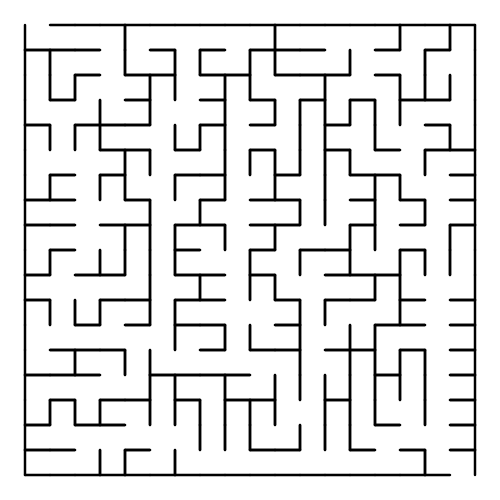
\includegraphics[scale=0.3]{img/maze.eps}
 \caption{A maze}
 \label{fig:maze}
\end{figure}

There are multiple methods to solve maze puzzle. We'll intorduce an effective, yet not the best one in this
section. There are some well known sayings about how to find the way out in maze, while not all of them are
true.

For example, one method states that, wherever you have multiple ways, always turn right. This doesn't work
as shown in figure \ref{fig:maze-loop}. The obvious solutoin is first to go along the top horizontal line,
then turn right,
and keep going ahead at the 'T' section. However, if we always turn right, we'll endless
loop around the inner big block.

\begin{figure}[htbp]
 \centering
 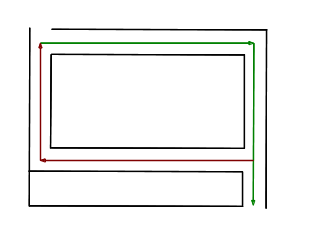
\includegraphics[scale=0.6]{img/maze-loop.eps}
 \caption{it leads to loop way if always turns right.}
 \label{fig:maze-loop}
\end{figure}

This example tells us that the decision when there are multiple choices matters the solution. Like the
fairy tale we read in our childhood, we can take some bread crumbs when walk in a maze, when there
are multiple ways, we can simply select one, left a piece of bread crumbs to mark this attempt as well
as the locations we've visited so far. If we enter a died end, we go back to the last place where
we've made a decision by back-tracking the bread crumbs. Then we can alter to another way. If the
bread crumbs show that all the ways have been tried, we must go back even further and try again.

At any time, if we find there have been already bread crumbs left, it means we have entered a loop, we
must go back and try different ways. Repeat these try-and-check steps, we can either find the way
out, or reveal the `no solution' fact. In the later case, we will back-track to the start point.

One easy way to describe a maze, is by a $m \times n$ matrix, each element is either 0 or 1, which
indicates if there is a way at this cell. The maze
illustrated in figure \ref{fig:maze-loop} can be defined as the following matrix.

\[
\begin{matrix}
0 & 0 & 0 & 0 & 0 & 0 \\
0 & 1 & 1 & 1 & 1 & 0 \\
0 & 1 & 1 & 1 & 1 & 0 \\
0 & 1 & 1 & 1 & 1 & 0 \\
0 & 1 & 1 & 1 & 1 & 0 \\
0 & 0 & 0 & 0 & 0 & 0 \\
1 & 1 & 1 & 1 & 1 & 0
\end{matrix}
\]

Given a start point $s=(i, j)$, and a goal $e=(p, q)$, we need find all solutions, that are the
paths from $s$ to $e$.

There is an obviously recursive exhaustive search method. That in order to find all paths from
$s$ to $e$, we can check all connected points to $s$, for every such point $k$, we recursively
find all paths from $k$ to $e$. This method can be illustrated as the following.

\begin{itemize}
\item Trivial case, if the start point $s$ is as same as the target point $e$, we are done;
\item Otherwise, for every connected point $k$ to $s$, recursively find the paths from $k$
to $e$; If $e$ can be reached via $k$, put section $s$-$k$ in front of each path between $k$
and $e$.
\end{itemize}

However, we have to left 'bread crumbs' to avoid repeatedly trying same attempts. This is because
otherwise in the recursive case, we start from $s$, find a connected point $k$, then we further
try to find paths from $k$ to $e$. Since $s$ is connected to $k$ as well, so in the next
recursion, we'll again try to find paths from $s$ to $e$. This ends up the very same origin
problem, and we are trapped in infinit recursions.

Our solution is to initialize an empty list, use it to record all the points we've visited so
far. For every connected points, we examine if it has already been visited by using this list.
We skip all the visited candidates and try those new ones. The coresponding algorithm can be
defined like this.

\be
solveMaze(m, s, e) = solve(s, \{ \Phi \})
\label{eq:solve-maze-reversed}
\ee

Where $m$ is the matrix which defines a maze, $s$ is the start point, and $e$ is the end point.
Function $solve$ is defined in the context of $solveMaze$, so that the maze and the end point
can be accessed. It can be realized recursively like what we described above\footnote{Function
$concat$ can flatten a list of lists. For example.
$concat(\{\{a, b, c\}, \{x, y, z\}\}) = \{a, b, c, x, y, z\}$. Refer to appendix A for detail.}.

\be
solve(s, P) = \left \{
  \begin{array}
  {r@{\quad:\quad}l}
  \{ \{ s\} \cup p | p \in P \} & s = e \\
  concat(\{ solve(s', \{ \{ s\} \cup p | p \in P \}) | \newline
  s' \in adjacent(s), \lnot visited(s')\}) & otherwise
  \end{array}
\right.
\ee

Note that $P$ also serves as an accumulator. Every connected point is recorded in all the
possible pahts to the current position. But they are stored in reversed order, that is
the newly visited point is put to the head of all the lists, and the start point is the last
element in these lists. This is because appending operation is linear ($O(n)$, where $n$ is
the number of elements stored in a list), while link to the head is just constant time
operation. We can output the result in correct order by reversing all possible solutions
in equation (\ref{eq:solve-maze-reverse})\footnote{the detailed defintion of $reverse$ can
be found in the appendix A.}

\be
solveMaze(m, s, e) = map(reverse, solve(s, \{ \Phi \}))
\ee

We need define functions $adjacent(p)$ and $visited(p)$, which finds all the connected
points to $p$, and test if point $p$ has been visited respectively. We only consider
two points are connected if and only if in the maze matrix they are next cells horizontally
or vertically, and both with value zero.

\be
\begin{array}{ll}
adjacent((x, y)) = \{ (x', y') | & (x', y') \in \{ (x-1, y), (x+1, y), (x, y-1), (x, y+1)\}, \\
 & 1 \leq x' \leq M, 1 \leq y' \leq N, m_{x' y'} = 0\} \\
\end{array}
\ee

Where $M$ and $N$ are the widths and heights of the maze.

Function $visited(p)$ just examine if point $p$ has been recoreded in any list in $P$.

\be
visited(p, P) = \exists path \in P, p \in path
\ee

The following Haskell example code implements this algorithm.

\lstset{language=Haskell}
\begin{lstlisting}
solveMaze m from to = map reverse $ solve from [[]] where
    solve p paths | p == to = map (p:) paths
                  | otherwise = concat [solve p' (map (p:) paths) |
                                        p' <- adjacent p, not $ visited p' paths]
    adjacent (x, y) = [(x', y') | (x', y') <- [(x-1, y), (x+1, y), (x, y-1), (x, y+1)],
                                  inRange (bounds m) (x', y'),
                                  m ! (x', y') == 0]
    visited p paths = any (p `elem`) paths
\end{lstlisting} %$

For a maze defined as a matrix like below example, all the solutions can be given
by this program.

\lstset{language=Haskell}
\begin{lstlisting}
mz = [[0, 0, 1, 0, 1, 1],
      [1, 0, 1, 0, 1, 1],
      [1, 0, 0, 0, 0, 0],
      [1, 1, 0, 1, 1, 1],
      [0, 0, 0, 0, 0, 0],
      [0, 0, 0, 1, 1, 0]]

maze  = listArray ((1,1), (6, 6)) . concat

solveMaze (maze mz) (1,1) (6, 6)
\end{lstlisting}

As we mentioned, this is a style of 'exhaustive search'. It recursively search all the connected
points as candidates. In a real maze solving game, a robot mouse competition for instance,
it's enough to just find a route. We can adapt to a method close to what described at the
begining of this section. That ask the robot mouse to try the first connected point, and won't
try others until it can't arrive the target location. We need some data structure to
store the 'bread crumbs', which help to remember the decisions being made. As we always attempt
to find the way on top of the latest decision, it's in the last-in, first-out manner. Which
indicate that we can use a stack.

At the very begining, only the starting point $s$ is stored in the stack. we pop it out,
find, for example, points $a$, and $b$, are connected to $s$, we push these two possible
paths: $\{a, s\}$ and $\{b, s\}$ to the stack. Next we pop $\{a, s\}$ out, and examine
connected points to $a$, if there are, all the 3-steps paths will be pushed back. We
repeat this process. At anytime, each element stored in the stack is a path, from the
starting point to the farest place this path can arrive in the reversed order.
This can be illustrated in figure \ref{fig:dfs-stack}.

\begin{figure}[htbp]
 \centering
 \includegraphics[scale=0.5]{img/dfs-stack.ps}
 \caption{The stack is intialized with a singleton list of the starting point $s$. $s$ is connected with point $a$ and $b$. Paths $\{a, s\}$ and $\{b, s\}$ are pushed back. In some step, the path ended with point $p$ is popped.
$p$ is connected with points $i$, $j$, and $k$. These 3 points are expanded as different options and pushed
back to the stack. The candidate path ended with $q$ won't be examined unless all the options above fail.}
 \label{fig:dfs-stack}
\end{figure}

The stack can be realized as a list, that the latest option is picked from the head, and new candidates are
added to the head. The maze puzzle can be solved by using such a list of paths:

\be
solveMaze'(m, s, e) = reverse(solve'(\{\{s\}\}))
\ee

As we are finding the first path, instead of all of them, $map$ isn't used here. When the stack is empty, it
means that we've tried all the options and failed to find a way out. The solution is therefore empty; otherwise,
the top option is popped, expanded with all the adajcent points which haven't been visited before, and pushed
back to the stack. Denote the stack as $S$, if it isn't empty, the top element is $s_1$, and the new stack
after the top is popped as $S'$. The top element $s_1$ is actually a path $P$, which is a list of points. Denote
the latest point in this path as $p_1$, and the rest of points as $P'$. The solution can be formalized as
the following.

\be
solve'(S) = \left \{
  \begin{array}
  {r@{\quad:\quad}l}
  \Phi & S = \Phi \\
  s_1 & s_1 = e \\
  solve'(S') & C = \{ c | c \in adjacent(p_1), c \not\in P' \} = \Phi \\
  solve'(\{ \{p\}\cup P | p \in C\} \cup S) & otherwise, C \neq \Phi
  \end{array}
\right.
\ee

Where the $adjacent$ function is defined above. This updated maze solution can be implemented with the
below example Haskell program \footnote{The same code of $adjacent$ function is skipped}.

\lstset{language=Haskell}
\begin{lstlisting}
dfsSolve m from to = reverse $ solve [[from]] where
    solve [] = []
    solve (c@(p:path):cs)
        | p == to = c -- stop at the first solution
        | otherwise = let os = filter (`notElem` path) (adjacent p) in
                          if os == []
                          then solve cs
                          else solve ((map (:c) os) ++ cs)
\end{lstlisting} %$

It's quite easy to modify this solution to another different version, which finds all possible
paths from the starting point to the end. When we found a solution in the second clause, instead
of returning this path, we record it and go on checking the rest memorized options in the stack
till all the possible ways are tried, which ends with an empty stack. We left it as an exercise to
the reader.

The same idea can also be realized imperatively. We maintain a stack to store all possible paths
begins from the starting point. In each iteration, the top option path is popped from the stack,
if the farest position is the end point, a solution is found; otherwise, all the adjacent, not
visited yet points are appended as new option paths and pushed back to the stack. This is repeated
till all the candidate paths in the stacks are checked, thus the stack ends up empty.

Use the same notation to represent the stack $S$. But the paths will be stored as arrays
instead of list in imperative settings as the former is more effective. Because of this
the starting point is the first element in the path array, while the farest reached
place is the right most element. We use $p_n$ to represent \textproc{Last}($P$) for
path $P$. The imperative algorithm can be given as below.

\begin{algorithmic}[1]
\Function{Solve-Maze}{$m, s, e$}
  \State $S \gets \Phi$
  \State \Call{Push}{$S, \{ s \}$}
  \State $L \gets \Phi$ \Comment{the result list}
  \While{$S \neq \Phi$}
    \State $P \gets$ \Call{Pop}{$S$}
    \If{$e = p_n$}
      \State \Call{Add}{$L, P$}
    \Else
      \For{$\forall p \in $ \Call{Adjacent}{$m, p_n$}}
        \If{$\lnot p \in P$}
          \State \Call{Push}{$S, P \cup \{ p \}$}
        \EndIf
      \EndFor
    \EndIf
  \EndWhile
  \State \Return $L$
\EndFunction
\end{algorithmic}

The following example Python program implements this maze solving algorithm.

\lstset{language=Python}
\begin{lstlisting}
def solve(m, src, dst):
    stack = [[src]]
    s = []
    while stack != []:
        path = stack.pop()
        if path[-1] == dst:
            s.append(path)
        else:
            for p in adjacent(m, path[-1]):
                if not p in path:
                    stack.append(path + [p])
    return s

def adjacent(m, p):
    (x, y) = p
    ds = [(0, 1), (0, -1), (1, 0), (-1, 0)]
    ps = []
    for (dx, dy) in ds:
        x1 = x + dx
        y1 = y + dy
        if 0 <= x1 and x1 < len(m[0]) and 0 <= y1 and y1 < len(m) and m[y][x] == 0:
            ps.append((x1, y1))
    return ps
\end{lstlisting}

And the same maze example given above can be solved by this program like the following.

\lstset{language=Python}
\begin{lstlisting}
mz = [[0, 0, 1, 0, 1, 1],
      [1, 0, 1, 0, 1, 1],
      [1, 0, 0, 0, 0, 0],
      [1, 1, 0, 1, 1, 1],
      [0, 0, 0, 0, 0, 0],
      [0, 0, 0, 1, 1, 0]]

solve(mz, (0, 0), (5,5))
\end{lstlisting}

It seems that in the worst case, there are 4 options (up, down, left, and right) at
each step, each option is pushed to the stack and eventually examined during backtracking.
Thus the complexity is bound to $O(4^n)$. The actual time won't be so big
because we filtered out the places which have been visited before.
In the worst case, all the reachable
points are visited exactly once. So the time is bound to $O(n)$, where $n$ is the
number of points connected in total. As a stack is used to store candidate solutions,
the space complexity is $O(n^2)$.

\subsubsection{8 queens puzzle}
Eight queeens puzzle is also a famous problem. Although cheese has very long history, this
puzzle was first published in 1848 by Max Bezzel\cite{wiki-8-queens}.
Queen in the cheese game is quite powerful.
It can attack any other pieces in the same row, column and diagonal at any distance within
the cheese board. The puzzle is to find ways to put 8 queens in the board, so that none of
them will attack each other. Figure \ref{fig:8-queens-puzzle} (a) illustrate the places can
be attacked by a queen and \ref{fig:8-queens-puzzle} (b) shows a solution of 8 queens puzzle.

\begin{figure}[htbp]
 \centering
 \subfloat[A queen piece.]{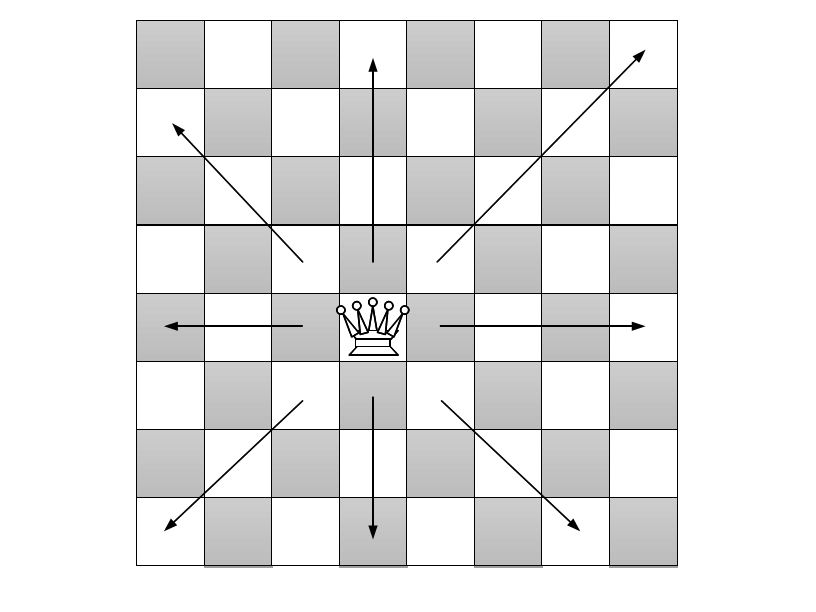
\includegraphics[scale=1]{img/queen.eps}}
 \subfloat[An example solution]{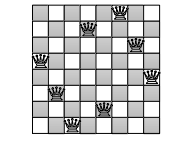
\includegraphics[scale=1]{img/queens-example.eps}}
 \caption{The eight queens puzzle.}
 \label{fig:8-queens-puzzle}
\end{figure}

It's obviously that this puzzle can be solved by brute-force, which takes $P^8_{64}$ times.
This number is about $4 \times 10^{10}$. This can be easily improved by observing that,
no two queens can be in the same row, and each queeen must be put on one column between
1 to 8. Thus we can represent a arrangement as a permutation of $\{1,2,3,4,5,6,7,8\}$.
For instance, arrangement $\{6,2,7,1,3,5,8,4\}$ means, we put the first queen at row 1,
column 6, the second queen at row 2 column 2, ..., and the last queen at row 8, column 4.
With this representation, we need only examine $8! = 40320$ possibilities.

We can find better solutions than this. Similar to the maze puzzle, we put queens one by
one from the first row. For the first queen, there are 8 options, that we can put it
at one of the eight columns. Then for the next queen, we again examine the 8 candidate
columns, some of them are not valid because those position will be attacked by the first
queen we've put, We repeat this process, for the $i$-th queen, we examine the 8 columns
in row $i$, find which columns are safe. If none column are valid, which means all the
columns in this row will be attacked by some queen we've previously arranged, we have
to backtrack as what we did in the maze puzzle. When all the 8 queens are successfully
put to the board, we find a solution. In order to find all the possible solutions, we
need record it and go on to examine other candidate columns and perform back track if
neccessary. This process ends when all the candidate columns in the first row have been
examined. The below equation starts the search.

\be
solve(\{\Phi\}, \Phi)
\ee

In order to manage the candidate attemptions, a stack $S$ can be used as same as in maze
puzzle. The stack is initialized with one empty element.
And a list $L$ is used to record all possible solutions.
Denote the top element in the stack as $s_1$. It's actually an intermediate state of
assignment, which is a partial permutation of 1 to 8.
after pop it, the stack is $S'$. The $solve$ function can be defined as the following.

\be
solve(S, L) = \left \{
  \begin{array}
  {r@{\quad:\quad}l}
  L & S = \Phi \\
  solve(S', \{s_1\} \cup L) & |s_1| = 8 \\
  solve(\{\{i\} \cup s_1| i \in [1,8], i \notin s_1, safe(i, s_1)\} \cup S', L) & otherwise
  \end{array}
\right.
\ee

If the stack is empty, it means all the possible candidates have been examined, It's not possilbe
to backtrack any more. $L$ has been accumulated all found solutions and returned as the result;
Otherwise, we pop the first candidate in the stack, if its length is 8, it means this candidate
is a valid solution. We record it by adding to $L$, and go on finding other solutions; If
its length is less than 8, we try to put the next queen. Among all the columns from 1 to 8, we
pick those not already occupied by previous queens (through the $i \notin s_1$ clause), and
must not be attacked in diagonal direction (through the $safe$ predication). These valid
assignments will be pushed to the stack for the further searching.

Function $safe(x, C)$ detects if the assigment of a queen in position $x$ will be attacked
by other queens in $C$ in diagonal direction. There are 2 possible cases, one is the
$45^{\circ}$ direction, the other is the $135^{\circ}$ dirction. Since the row of this new
queen is $y = 1 + |C|$, where $|C|$ is the length of $C$, the $safe$ function can be
defined as the following.

\be
safe(x, C) = \forall (c, r) \in zip(reverse(C), \{1, 2, ...\}), |x - c| \neq |y - r|
\ee

Where $zip$ takes two lists, and pairs every elements in them to a new list. Thus
If $C = \{ c_{i-1}, c_{i-2}, ..., c_2, c_1\}$ represents the column of the first $i-1$
queens has been assigned, the above function will check list of pairs
$\{(c_1, 1), (c_2, 2), ..., (c_{i-1}, i-1)\}$ with position $(x, y)$ form any
diagonal line.

Translate this algorithm into Haskell gives the below example program.

\lstset{language=Haskell}
\begin{lstlisting}
solve = dfsSolve [[]] [] where
    dfsSolve [] s = s
    dfsSolve (c:cs) s
             | length c == 8 = dfsSolve cs (c:s)
             | otherwise = dfsSolve ([(x:c) | x <- [1..8] \\ c,
                               not $ attack x c] ++ cs) s
    attack x cs = let y = 1 + length cs in
                  any (\(c, r) -> abs(x - c) == abs(y - r)) $
                      zip (reverse cs) [1..]
\end{lstlisting}

Observing that the algorithm is tail recursive, it's easy to transform it into
imperative one. Instead of using list, we use array to represent queens assignment.
Denote the stack as $S$, and the possible solutions as $A$. The imperative
algorithm can be described as the following.

\begin{algorithmic}[1]
\Function{Solve-Queens}{}
  \State $S \gets \{\Phi\}$
  \State $L \gets \Phi$ \Comment{The result list}
  \While{$S \neq \Phi$}
    \State $A \gets$ \Call{Pop}{$S$} \Comment{$A$ is an intermediate assignment}
    \If{$|A|=8$}
      \State \Call{Add}{$L, A$}
    \Else
      \For{$i \gets 1$ to $8$}
        \If{\Call{Valid}{$i, A$}}
          \State \Call{Push}{$S, A \cup \{i\}$}
        \EndIf
      \EndFor
    \EndIf
  \EndWhile
  \State \Return $L$
\EndFunction
\end{algorithmic}

The stack is initialized with an empty assignment. The main process repeatedly
pops the top candidate from the stack, If there are still queens left, the algorithm
examines possible columns in the next row from 1 to 8, if a column is safe, that
it won't be attacked by any previous queens, this column will be appended
to the assignment, and pushed back to the stack. Different from the functional
approach, since array, but not list, is used, we simply record the solution
when the length of the assignment array is 8 without reverse it.

Function \textproc{Valid} check if column $x$ is safe with some queens put
according to $A$. It filters the columns have already occupied out, and calulate
if any diagonal lines are formed with existing queens.

\begin{algorithmic}[1]
\Function{Valid}{$x, A$}
  \State $y \gets 1 + |A|$
  \For{$i \gets 1$ to $|A|$}
    \If{$x = i \lor |y-i| = |x - A[i]|$}
      \State \Return False
    \EndIf
  \EndFor
  \State \Return True
\EndFunction
\end{algorithmic}

The following Python example program implements this imperative algorithm.

\lstset{language=Python}
\begin{lstlisting}
def solve():
    stack = [[]]
    s = []
    while stack != []:
        a = stack.pop()
        if len(a) == 8:
            s.append(a)
        else:
            for i in range(1, 9):
                if valid(i, a):
                    stack.append(a+[i])
    return s

def valid(x, a):
    y = len(a) + 1
    for i in range(1, y):
        if x == a[i-1] or abs(y - i) == abs(x - a[i-1]):
            return False
    return True
\end{lstlisting}

Although there are 8 optional columns when assign eash queen, but not all of them
are valid and thus further expanded. Only those columns haven't been occupied by
previous queens are attempted. The algorithm only examines 15720, which is far
less than $8^8 = 16777216$ possibilities \cite{wiki-8-queens}.

It's quite easy to extend the algorithm, so that it can solve $N$ queens puzzle, where
$N \geq 4$, although the time cost increase fast. The backtrack algorithm is just
slightly better than the one permunate the sequence of 1 to 8 (which is bound to $o(N!)$).
Another extension to the algorithm is based on the fact that the chess board is
square, which is symmetric both vertically and horizontally. Thus a solution can
generate other solutions by rotate it or flip it. These 2 aspects are left as
exercises to the reader.

\subsubsection{Peg puzzle}
I onced received a puzzle of the leap frogs. It said to be homework
for 2nd grade student in China. As illustrated in figure \ref{fig:leapfrog}, there
are 6 frogs in 7 stones. Each frog can either hop to the next stone if it is not
occupied, or leap over one frog to another empty stone. The frogs on the left side
can only move to the right, while the ones on the right side can only move to the
left. These rules are described in figure \ref{fig:pegrules}

\begin{figure}[htbp]
 \centering
 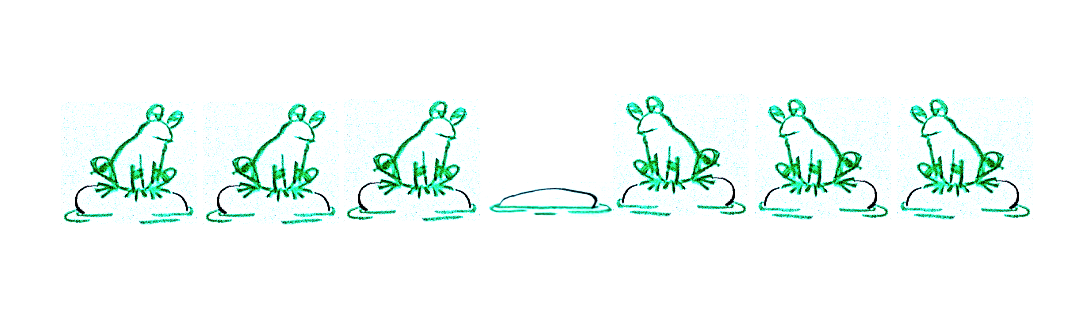
\includegraphics[scale=0.4]{img/leapfrogs.eps}
 \caption{The leap frogs puzzle.}
 \label{fig:leapfrog}
\end{figure}

The goal of these puzzle is to arrange the frogs to jump according to the rules, so
that the positions of the left 3 frogs are finaly exchange with the 3 on the right.
If we denote the left frog as 'A', the right as 'B', the empty stone as 'O'. The
puzzle is to find a solution to transform from 'AAAOBBB' to 'BBBOAAA' according
to the moving rules.

\begin{figure}[htbp]
 \centering
 \subfloat[Jump to the next stone]{
\includegraphics[scale=0.3]{img/leapfrog1.eps}} \hspace{0.02\textwidth}
 \subfloat[Jump over to the right]{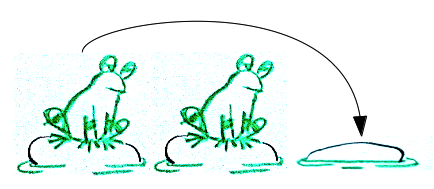
\includegraphics[scale=0.3]{img/leapfrog2.eps}} \hspace{0.02\textwidth}
 \subfloat[Jump over to the left]{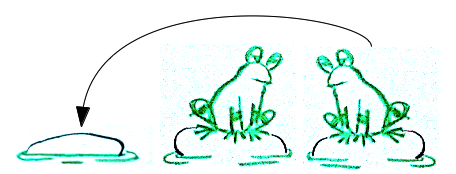
\includegraphics[scale=0.3]{img/leapfrog3.eps}}
 \caption{Moving rules.}
 \label{fig:pegrules}
\end{figure}

This puzzle is just a special form of the peg puzzles. The number of pegs are not
limited to 6. it can be 8 or even bigger even numbers. Figure \ref{fig:pegpuzzles}
shows some variants.

\begin{figure}[htbp]
 \centering
 \subfloat[Solitaire]{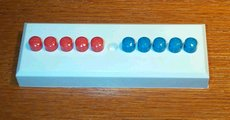
\includegraphics[scale=0.5]{img/solitaire.eps}} \hspace{0.02\textwidth}
 \subfloat[Hop over]{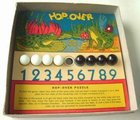
\includegraphics[scale=0.7]{img/hop-over.eps}} \hspace{0.02\textwidth}
 \subfloat[Draught board]{
\includegraphics[scale=0.3]{img/draught-board.eps}}
 \caption{Variants of the peg puzzles from http://home.comcast.net/~stegmann/jumping.htm}
 \label{fig:pegpuzzles}
\end{figure}

We can solve this puzzle by computer program. The idea is similar to the 8 queens puzzle.
Denote the position from the left most stone as 1, 2, ..., 7.
In ideal cases, there are 4 options to arrange the move. For example when start, the frog
on 3rd stone can hop right to the empty stone; symmetrically, the frog on the 5th stone
can hop left; Alternatively, the frog on the 2nd stone can leap right, while the frog on
the 6th stone can leap left.

We can record the state and try one of these 4 options at every step. Of course not all of them
are possible at any time. If get stuck, we can backtrack and try other options.

As we restrict the left side frogs only move to the right, and the right frogs only
move to the left. The moves are not reversable. There won't be any repeatation cases as
what we have to deal with in the maze puzzle. However, we still need record the steps
in order to print them out finally.

In order to enforce these restriction, let A, O, B in representation 'AAAOBBB' be -1, 0,
and 1 repectively. A state $L$ is a list of elements, each elements is one of these 3
values. It starts from $\{-1, -1, -1, 0, 1, 1, 1\}$. $L[i]$ access the $i$-th element,
its value means if the $i$-th stone is empty, occupied by a frog from left side, or
occupied by a frog from right side. Denote the position of the vacant stone as $p$.
The 4 moving options can be stated as below.

\begin{itemize}
\item Leap left: $p < 6$ and $L[p+2] > 0$, swap $L[p] \leftrightarrow L[p+2]$;
\item Hop left: $p < 7$ and $L[p+1] > 0$, swap $L[p] \leftrightarrow L[p+1]$;
\item Leap right $p > 2$ and $L[p-2] < 0$, swap $L[p-2] \leftrightarrow L[p]$;
\item Hop right $p > 1$ and $L[p-1] < 0$, swap $L[p-1] \leftrightarrow L[p]$.
\end{itemize}

Four functions $leap_l(L), hop_l(L), leap_r$ and $hop_r(L)$ are defined accordingly.
If the state $L$ does not satisfy the move restriction, these function return $L$
unchanged, otherwise, the changed state $L'$ is given accordingly.

We can also explicityly maintain a stack $S$, which stores the attemptation as
well as the historic movements. The stack is initilaized with a singleton list
of start state. The solution is put to a list $M$, which is empty at the begining:

\be
solve(\{\{-1, -1, -1, 0, 1, 1, 1\}\}, \Phi)
\ee

As far as the stack isn't empty, we pop one possible itermediate attemptation. If
the latest state is equal to $\{1, 1, 1, 0, -1, -1, -1\}$, a solution is found,
we append the series of moves till this state to the result list $M$; otherwise,
We expand to next possible state by trying all four possible moves, and push
them back to the stack for further search. Denote the top element in the stack
$S$ as $s_1$, and the lastest state in $s_1$ as $L$. The algorithm can be
defined as the following.

\be
solve(S, M) = \left \{
  \begin{array}
  {r@{\quad:\quad}l}
  M & S = \Phi \\
  solve(S', \{reverse(s_1)\} \cup M) & |L| = \{1, 1, 1, 0, -1, -1, -1\} \\
  solve(P \cup S', M) & otherwise
  \end{array}
\right.
\ee

Where $P$ are possible moves from the latest state $L$, that
\[
P = \{ L'  | L' \in \{leap_l(L), hop_l(L), leap_r(L), hop_r(L)\}, L \neq L'\}
\]

Note that the start state is stored as the last element, while the
final state is stored as the first, that's why we reverse it when add
to solution list.

Translating this algorithm to Haskell gives the following example program.

\lstset{language=Haskell}
\begin{lstlisting}
solve = dfsSolve [[[-1, -1, -1, 0, 1, 1, 1]]] [] where
    dfsSolve [] s = s
    dfsSolve (c:cs) s
             | head c == [1, 1, 1, 0, -1, -1, -1] = dfsSolve cs (reverse c:s)
             | otherwise = dfsSolve ((map (:c) $ moves $ head c) ++ cs) s

moves s = filter (/=s) [leapLeft s, hopLeft s, leapRight s, hopRight s] where
    leapLeft [] = []
    leapLeft (0:y:1:ys) = 1:y:0:ys
    leapLeft (y:ys) = y:leapLeft ys
    hopLeft [] = []
    hopLeft (0:1:ys) = 1:0:ys
    hopLeft (y:ys) = y:hopLeft ys
    leapRight [] = []
    leapRight (-1:y:0:ys) = 0:y:(-1):ys
    leapRight (y:ys) = y:leapRight ys
    hopRight [] = []
    hopRight (-1:0:ys) = 0:(-1):ys
    hopRight (y:ys) = y:hopRight ys
\end{lstlisting}

Running this program finds 2 symmetric solution, each takes 15 steps. One solution
is list in the below table.

\begin{tabular}{|c||c|c|c|c|c|c|c|}
\hline
step & -1 & -1 & -1 & 0 & 1 & 1 & 1 \\
1 & -1 & -1 & 0 & -1 & 1 & 1 & 1 \\
2 & -1 & -1 & 1 & -1 & 0 & 1 & 1 \\
3 & -1 & -1 & 1 & -1 & 1 & 0 & 1 \\
4 & -1 & -1 & 1 & 0 & 1 & -1 & 1 \\
5 & -1 & 0 & 1 & -1 & 1 & -1 & 1 \\
6 & 0 & -1 & 1 & -1 & 1 & -1 & 1 \\
7 & 1 & -1 & 0 & -1 & 1 & -1 & 1 \\
8 & 1 & -1 & 1 & -1 & 0 & -1 & 1 \\
9 & 1 & -1 & 1 & -1 & 1 & -1 & 0 \\
10 & 1 & -1 & 1 & -1 & 1 & 0 & -1 \\
11 & 1 & -1 & 1 & 0 & 1 & -1 & -1 \\
12 & 1 & 0 & 1 & -1 & 1 & -1 & -1 \\
13 & 1 & 1 & 0 & -1 & 1 & -1 & -1 \\
14 & 1 & 1 & 1 & -1 & 0 & -1 & -1 \\
15 & 1 & 1 & 1 & 0 & -1 & -1 & -1 \\
\hline
\end{tabular}

Observe that the algorithm is in tail recursive manner, it can also be realized imperatively
in a straightforward way. The algorithm can also be more generalized, so that it can be
used to solve the puzzle that there are $n$ frogs on each side. We represent the start
state \{-1, -1, ..., -1, 0, 1, 1, ..., 1\} as $s$, and the mirrored end state as $e$.

\begin{algorithmic}[1]
\Function{Solve}{$s, e$}
  \State $S \gets \{\{s\}\}$
  \State $M \gets \Phi$
  \While{$S \neq \Phi$}
    \State $s_1 \gets$ \Call{Pop}{$S$}
    \If{$s_1[1] = e$}
      \State \textproc{Add}($M$, \Call{Reverse}{$s_1$})
    \Else
      \For{$\forall m \in$ \Call{Moves}{$s_1[1]$}}
        \State \textproc{Push}($S$, $\{m\} \cup s_1$)
      \EndFor
    \EndIf
  \EndWhile
  \State \Return $M$
\EndFunction
\end{algorithmic}

The possible moves can be also generalized to handle arbitrary frogs. The following
Python program implements this generalized solution.

\lstset{language=Python}
\begin{lstlisting}
def solve(start, end):
    stack = [[start]]
    s = []
    while stack != []:
        c = stack.pop()
        if c[0] == end:
            s.append(reversed(c))
        else:
            for m in moves(c[0]):
                stack.append([m]+c)
    return s

def moves(s):
    ms = []
    n = len(s)
    p = s.index(0)
    if p < n - 2 and s[p+2] > 0:
        ms.append(swap(s, p, p+2))
    if p < n - 1 and s[p+1] > 0:
        ms.append(swap(s, p, p+1))
    if p > 1 and s[p-2] < 0:
        ms.append(swap(s, p, p-2))
    if p > 0 and s[p-1] < 0:
        ms.append(swap(s, p, p-1))
    return ms

def swap(s, i, j):
    a = s[:]
    (a[i], a[j]) = (a[j], a[i])
    return a
\end{lstlisting}

For 3 frogs in one side, we know that it takes 15 steps to exchange them.
It's interesting to examine the table that how many steps need to exchange
the frogs along with the number of frogs in each side. Drive the example
program gives the following result.

\begin{tabular}{c|c|c|c|c|c|c}
number of frogs & 1 & 2 & 3  & 4  & 5 & ... \\
\hline
number of steps & 3 & 8 & 15 & 24 & 35 & ...
\end{tabular}

It seems that the number of steps are all square numbers minus one.
It's natural to guess that the number of steps for $n$ frogs in one side is
$(n+1)^2 - 1$. Actually we can prove it's true.

Compare to the final state and the start state, each frog moves ahead $n+1$
stones in its opposite direction. Thus total $2n$ frogs moves $2n(n+1)$ stones.
Another important fact is that each frog on the left has to meet every one
on the right one time, where leap will happen if meets. The frog moves two
stones ahead by leap. There are total $n^2$ meets happen, so that all these
meets cause moving $2n^2$ stones ahead. The rest moves are not leap, but hop.
The number of hops are $2n(n+1) - 2n^2 = 2n$. Sum up all $n^2$ leaps and $2n$
hops, the total number of steps are $n^2 + 2n = (n+1)^2 -1$.

\subsubsection{Summary of DFS}
Observe the above three puzzles, although they vary in many aspects, their
solutions show quite similar common structures. They all have some starting
state. The maze starts from the entrence point; The 8 queens puzzle starts
from the empty board; The leap frogs start from the state of 'AAAOBBB'.
The solution is a kind of searching, at each attemptation, there are several
possible ways. For the maze puzzle, there are four different directions to try;
For the 8 queens puzzle, there are eight columns to choose; For the leap
frogs puzzle, there are four movements of leap or hop. We don't know how
far we can go when make a decision, although the final state is clear.
For the maze, it's the exit point; For the 8 queens puzzle, we are done
when all the 8 queens being assigned on the board; For the leap frogs
puzzle, the final state is that all frogs exchanged.

We use a common approach to solve them. We repeatedly select one possible
candidate to try, record where we've achieved; If we get stuck, we backtrack
and try other options. We are sure by using this strategy, we can either
find a solutoin, or tell that the problem is unsolvable.

Of course there can be some variation, that we can stop when find an answer,
or go on finding all the possible solutions.

If we draw a tree rooted at the starting state, expand it so that every
branch stands for a different attemptation, our solution searching process
is in a manner, that we search deeper and deeper. We won't consider any
other options in the same depth unless the searching fails so that we've
to backtrack to upper level of the tree. Figure \ref{fig:dfs-tree} illustrates
the order we search a state tree. The arrow indicates how we go down
and backtrack up. The number of the nodes is the order we visit them.

\begin{figure}[htbp]
 \centering
 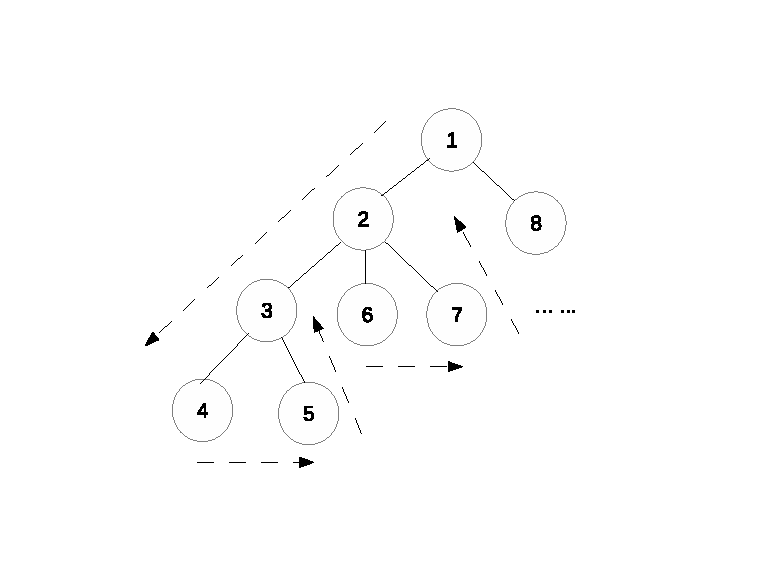
\includegraphics[scale=0.5]{img/dfs-tree.eps}
 \caption{Example of DFS search order.}
 \label{fig:dfs-tree}
\end{figure}

This kind of search strategy is called 'DFS' (Deep-first-search). We widely
use it unintentionally. Some programming environment, Prolog for instance,
adopt DFS as the default evaluation model. If a maze is given by a set
of rule base, such as:

\lstset{language=Prolog}
\begin{lstlisting}
c(a, b). c(a, e).
c(b, c). c(b, f).
c(e, d), c(e, f).
c(f, c).
c(g, d). c(g, h).
c(h, f).
\end{lstlisting}

Where predicate $c(X, Y)$ means place $X$ is connected with $Y$. Note that
this is a directed predicate, we can make $Y$ is connected with $X$ as well
by either adding a symmetric rule, or create a undirected predicate. Figure
\ref{fig:directed-graph} shows such a directed graph. Given two places $X$ and $Y$, prolog can
tell if they are connected by the following program.

\begin{figure}[htbp]
 \centering
 \includegraphics[scale=0.5]{img/directed-graph.ps}
 \caption{A directed graph.}
 \label{fig:directed-graph}
\end{figure}

\lstset{language=Prolog}
\begin{lstlisting}
go(X, X).
go(X, Y) :- c(X, Z), go(Z, Y)
\end{lstlisting}

This program says that, a place is connected with itself. If given two different places $X$ and
$Y$, if $X$ is connected with $Z$, and $Z$ is connected with $Y$, then $X$ is connected with $Y$.
Note that, there might be multiple choices for $Z$. Prolog choses a candidate, and go on further
searching. It only tries other candidates if the recursive searching fails. In that case, Prolog
backtracks and tries other alternatives. This is exactly what DFS does.

DFS is quite straightforward when we only need a solution, but don't care if it the solution takes
fewest steps. For example, the solution it gives, may not be the shortest path for the maze. We'll
see some more puzzles next. They need find the solution with minimum attempts.


\subsubsection{The wolf, goat, and cabbage puzzle}
This puzzle says that a farmer wants to cross a river with a wolf, a goat, and a bucket of cabbage.
There is a boat. Only the farmer can drive it. But the boat is small. it can only hold one of the
wolf, the goat, and the bucket of cabbage with the farmer at a time. The farmer has to pick
them one by one to the other side of the river. However, the wolf would eat the goat, and the
goat would eat the cabbage if the farmer is absent. The puzzle asks to find the fast solution
so that they can all safely go cross the river.

\begin{figure}[htbp]
 \centering
 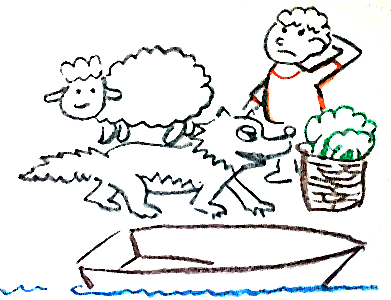
\includegraphics[scale=0.3]{img/wgc-puzzle.eps}
 \caption{The wolf, goat, cabbage puzzle}
 \label{fig:wgc-puzzle}
\end{figure}

The key point to this puzzle is that the wolf does not eat the cabbage. The farmer can safely
pick the goat to the other side. But next time, no matter if he pick the wolf or the cabbage
to cross the river, he has to take one back to avoid the confliction. In order to find the
fast the solution, at any time, if the farmer has multiple options, we can examine all of them
in parallel, so that these different decisions compete. If we count the number of the
times the farmer cross the river without considering the direction, that crossing the river
back and forth means 2 times, we are actually checking the complete possibilities after 1 time,
2 times, 3 times, ... When we find a situation, that they all arrive the other bank,
we are done. And this solution wins the compete, which is the fast solution.

The problem is that we can't really examine all possible solutions in parrallel ideally.
Even with a super computer equipped with many CPU cores, the setup is too expensive to
solve such a simple puzzle.

Let's consider a lucky draw game. People blindly pick from a box with colored balls. There
is only one black ball, all the others are white. The one who pick the black ball wins the
game; Otherwise, he must return the ball to the box and wait for the next chance.
In order to be fair enough, we can setup a rule that no one can try the second time before
all others have tried. We can line people to a queue. Every time the first guy
pick a ball, if he does not win, he then stands at the tail of the queue to wait for the
second try. This queue helps to ensure our rule.

\begin{figure}[htbp]
 \centering
 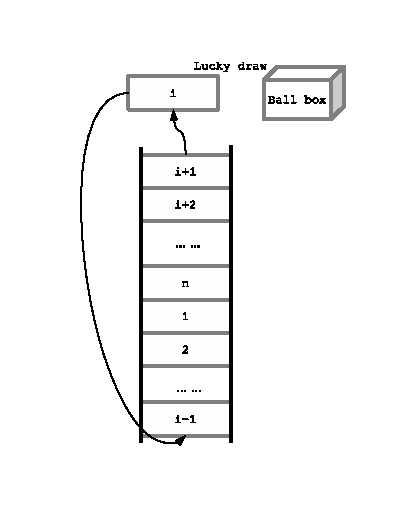
\includegraphics[scale=1]{img/lucky-draw.eps}
 \caption{A lucky-draw game, the $i$-th person goes from the queue, pick a ball, then join the queue at tail if he fails to pick the black ball.}
 \label{fig:luck-draw}
\end{figure}

We can use the quite same idea to solve our puzzle. The two banks of the river can be
represented as two sets $A$ and $B$. $A$ contains the wolf, the goat, the cabbage and
the farmer; while $B$ is empty. We take an element from one set to the other
each time. The two sets can't hold conflict things if the farmer is absent. The goal is
to exchange the contents of $A$ and $B$ with fewest steps.

We intialize a queue with state $A = \{w, g, c, p\}, B=\Phi$ as the only element.
As far as the queue isn't empty, we pick the first element from the head, expand it
with all possible options, and put these new expanded candidates to the tail of the queue.
If the first element on the head is the final goal, that $A=\Phi, B=\{w, g, c, p\}$,
we are done. Figure \ref{fig:bfs-tree} illustrates the idea of this search order.
Note that as all possibilites in the same level are examined, there is no need for
back-tracking.

\begin{figure}[htbp]
 \centering
 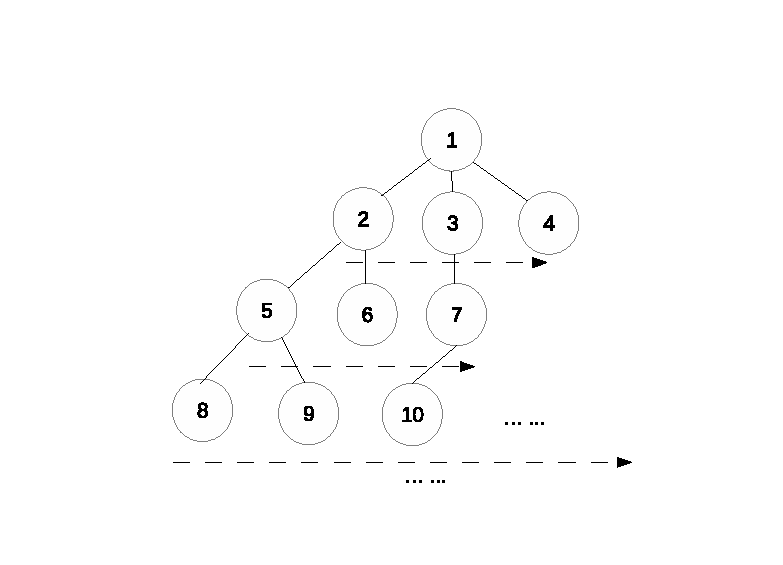
\includegraphics[scale=0.5]{img/bfs-tree.eps}
 \caption{Start from state 1, check all possible options 2, 3, and 4 for next step; then all nodes in level 3, ...}
 \label{fig:bfs-tree}
\end{figure}

There is a simple way to treat the set. A four bits binary number can be used, each
bit stands for a thing, for example, the wolf $w=1$, the goat $g=2$, the cabbate
$c=4$, and the farmer $p=8$. That 0 stands for the empty set, 15 stands for a
full set. Value 3, solely means there are a wolf and a goat on the river bank. In
this case, the wolf will eat the goat. Simliarily, value 6 stands for another
conflicting case. Every time, we move the highest bit (which is 8), or together
with one of the other bits (4 or 2, or 1) from one number to the other. The
possilbe moves can be defined as below.

\be
mv(A, B) = \left \{
  \begin{array}
  {r@{\quad:\quad}l}
  \{(A - 8 - i, B + 8 + i) | i \in \{0, 1, 2, 4\}, i = 0 \lor A \overline{\land} i \neq 0 \} & B < 8 \\
  \{(A + 8 + i, B - 8 - i) | i \in \{0, 1, 2, 4\}, i = 0 \lor B \overline{\land} i \neq 0 \} & Otherwise
  \end{array}
\right.
\ee

Where $\overline{\land}$ means bitwise and operation.

the solution can be given by reusing the queue defined in previous chapter. Denote
the queue as $Q$, which is initialed with a singleton list \{(15, 0)\}. If $Q$ is
not empty, function $DeQ(Q)$ extracts the head element $M$, the updated queue
becomes $Q'$. $M$ is a list of pairs, stands for a series of movements between the
river banks. The first element in $m_1=(A', B')$ is the latest state. Function
$EnQ'(Q, L)$ push all possible moving sequence in $L$ to the tail of the
queue one by one and returns the updated queue.
With these notations, the solution funciton is defined like below.

\be
solve(Q) = \left \{
  \begin{array}
  {r@{\quad:\quad}l}
  \Phi & Q = \Phi \\
  reverse(M) & A' = 0 \\
  solve(EnQ'(Q', \{\{m\} \cup M| m \in mv(m_1), valid(m, M)\})) & otherwise
  \end{array}
\right.
\ee

Where function $valid(m, M)$ check new moving candidate $m=(A'', B'')$ is valid.
That neither $A''$ nor $B''$ is 3 or 6, and $m$ hasn't been tried before in $M$,
so that to avoid any repeatedly attemptations.

\be
valid(m, M) = A'' \neq 3, A'' \neq 6, B'' \neq 3, B'' \neq 6, m \notin M
\ee

The following example Haskell program implements this solution. Note that it
uses a plain list to represent the queue for illustration purpose.

\lstset{language=Haskell}
\begin{lstlisting}
import Data.Bits

solve = bfsSolve [[(15, 0)]] where
    bfsSolve :: [[(Int, Int)]] -> [(Int, Int)]
    bfsSolve [] = [] -- no solution
    bfsSolve (c:cs) | (fst $ head c) == 0 = reverse c
                    | otherwise = bfsSolve (cs ++ map (:c)
                                      (filter (`valid` c) $ moves $ head c))
    valid (a, b) r = not $ or [ a `elem` [3, 6], b `elem` [3, 6], (a, b) `elem` r]

moves (a, b) = if b < 8 then trans a b else map swap (trans b a) where
    trans x y = [(x - 8 - i, y + 8 + i)
                     | i <-[0, 1, 2, 4], i == 0 || (x .&. i) /= 0]
    swap (x, y) = (y, x)
\end{lstlisting}

This algorithm can be easily modified to find all the possible solutions, but
not just stop when find the first one. This is left as an exercise to the
reader. The following are the only two solutions for this puzzle.

Solution 1:

\begin{tabular}{l|c|l}
Left & river & Right \\
\hline
wolf, goat, cabbage, farmer &   & \\
wolf, cabbage &   & goat, farmer \\
wolf, cabbage, farmer &   & goat \\
cabbage &   & wolf, goat, farmer \\
goat, cabbage, farmer &   & wolf \\
goat &   & wolf, cabbage, farmer \\
goat, farmer &   & wolf, cabbage \\
 &  & wolf, goat, cabbage, farmer
\end{tabular}

Solution 2:

\begin{tabular}{l|c|l}
Left & river & Right \\
\hline
 wolf, goat, cabbage, farmer & & \\
 wolf, cabbage & & goat, farmer \\
 wolf, cabbage, farmer & & goat \\
 wolf & & goat, cabbage, farmer \\
 wolf, goat, farmer & & cabbage \\
 goat & & wolf, cabbage, farmer \\
 goat, farmer & & wolf, cabbage \\
 & & wolf, goat, cabbage, farmer
\end{tabular}

This algorithm can also be realized imperatively. Observing that our
solution is in tail recursive manner, we can translate it directly
to a loop. We use a list $S$ to hold all the solutions can be found.
The singleton list $\{(15, 0)\}$ is pushed to queue when initializing.
As long as the queue isn't empty, we extract the head $C$ from the
queue by calling \textproc{DeQ} procedure. Examine if it reaches the
final goal, if not, we expand all possible moves and push to the
tail of the queue for further searching.

\begin{algorithmic}[1]
\Function{Solve}{}
  \State $S \gets \Phi$
  \State $Q \gets \Phi$
  \State \Call{EnQ}{$Q, \{(15, 0)\}$}
  \While{$Q \neq \Phi$}
    \State $C \gets $ \Call{DeQ}{$Q$}
    \If{$c_1 = (0, 15)$}
      \State \textproc{Add}($S$, \Call{Reverse}{$C$})
    \Else
      \For{$\forall m \in $ \Call{Moves}{$C$}}
        \If{\Call{Valid}{$m, C$}}
          \State \Call{EnQ}{$Q, \{m\} \cup C$}
        \EndIf
      \EndFor
    \EndIf
  \EndWhile
  \State \Return $S$
\EndFunction
\end{algorithmic}

Where \textproc{Moves}, and \textproc{Valid} procedures are as
same as before. The following Python example program implements
this imperative algorithm.

\lstset{language=Python}
\begin{lstlisting}
def solve():
    s = []
    queue = [[(0xf, 0)]]
    while queue != []:
        cur = queue.pop(0)
        if cur[0] == (0, 0xf):
            s.append(reverse(cur))
        else:
            for m in moves(cur):
                queue.append([m]+cur)
    return s

def moves(s):
    (a, b) = s[0]
    return valid(s, trans(a, b) if b < 8 else swaps(trans(b, a)))

def valid(s, mv):
    return [(a, b) for (a, b) in mv
        if a not in [3, 6] and b not in [3, 6] and (a, b) not in s]

def trans(a, b):
    masks = [ 8 | (1<<i) for i in range(4)]
    return [(a ^ mask, b | mask) for mask in masks if a & mask == mask]

def swaps(s):
    return [(b, a) for (a, b) in s]
\end{lstlisting}

There is a minor difference between the program and the code, that the function
to generate candidate moving options filters the invalid cases inside it.

Every time, no matter the farmer drives the boat back and forth, there are
$m$ options for him to choose, where $m$ is the number of objects on the
river bank the farmer drives from. $m$ is always less than 4, that the
algorithm won't take more than $n^4$ times at step $n$. This estimation
is far more than the actual time, because we avoid trying all invalid
cases. Our solution examines all the possible moving in the worst case.
Because we check recorded steps to avoid repeated attemptations, the
algorithm takes about $O(n^2)$ time to search $n$ possible moving.

\subsubsection{Water jugs puzzle}
This is a popular puzzle in classic AI. The history of it should be very long.
It says that there are only two jugs, one is 9 quarts jug, the other is 4 quarts
jug. How to use them to bring up from the river exactly 6 quarts of water?

Thera are varies versions of this kind of puzzle, although the volume
of the jugs, and the target volume of water differs. The solver is said to
be young Blaise Pascal when he was a child, the French mathematican,
scientist in one story, and Sim\`{e}on Denis Poisson in another story.
Later in the popular Hollywood movie `Die-Hard 3', actor Bruce Willis
and Samuel L. Jackson were also confronted with this puzzle.

P\`{o}lya gave a nice way to solve this problem backwards in \cite{how-to-solve-it}.

\begin{figure}[htbp]
 \centering
 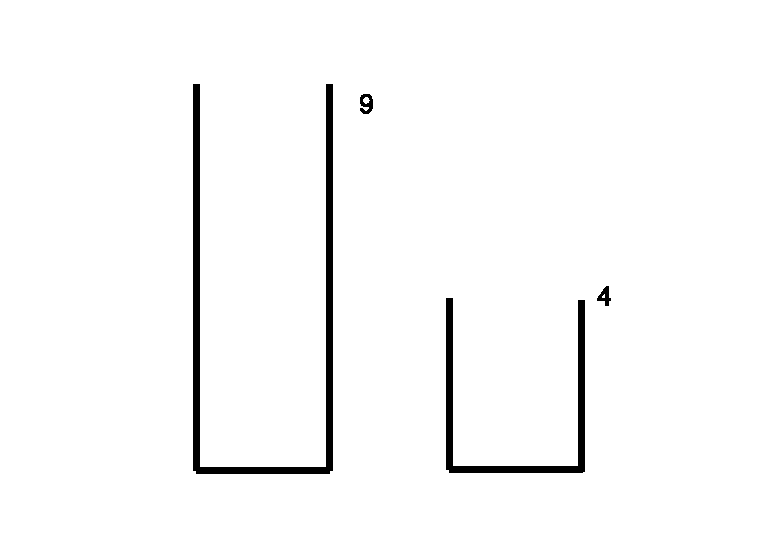
\includegraphics[scale=0.5]{img/jugs-start.eps}
 \caption{Two jugs with volume of 9 and 4.}
 \label{fig:jugs-start}
\end{figure}

Instead of thinking from the start state as shown in figure \ref{fig:jugs-start}.
P\`{o}lya pointed out that there will be 6 quarts of water in the bigger jugs
at the final stage, which indicats the last second step, we can fill the
9 quarts jug, then pour out 3 quarts from it. In order to achieve this, there
should be 1 quart of water left in the smaller jug as shown in figure
\ref{fig:jugs-r1}.

\begin{figure}[htbp]
 \centering
 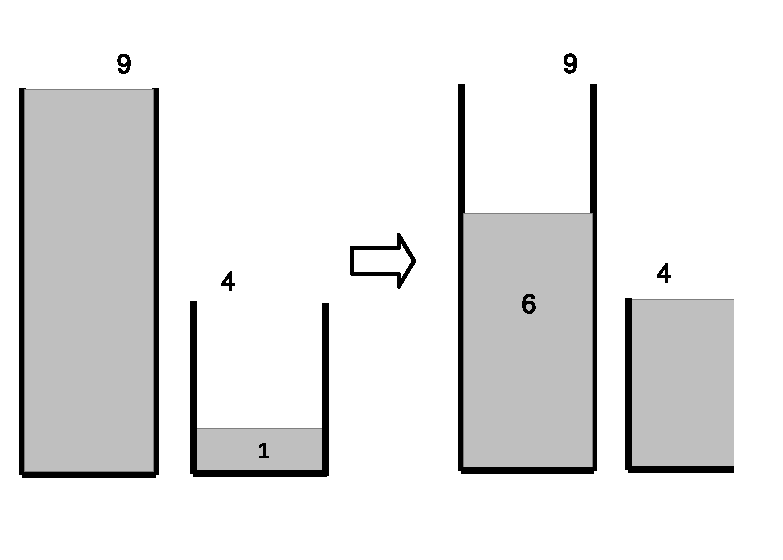
\includegraphics[scale=0.5]{img/jugs-r1.eps}
 \caption{The last two steps.}
 \label{fig:jugs-r1}
\end{figure}

It's easy to see that fill the 9 quaters jug, then pour to the 4 quaters
jug twice can bring 1 quaters of water. As shown in figure \ref{fig:jugs-r2}.
At this stage, we've found the solution. By reversing our findings, we
can give the correct steps to bring exactly 6 quaters of water.

\begin{figure}[htbp]
 \centering
 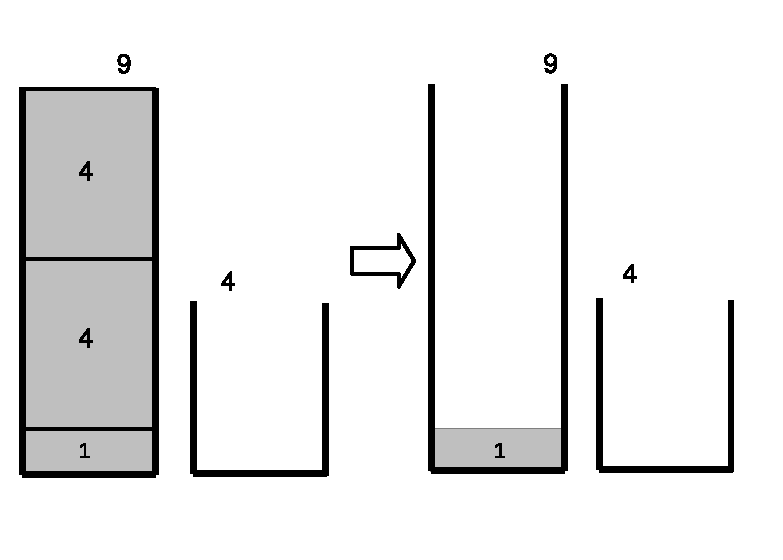
\includegraphics[scale=0.5]{img/jugs-r2.eps}
 \caption{Fill the bigger jugs, and pour to the smaller one twice.}
 \label{fig:jugs-r2}
\end{figure}

P\`{o}lya's methodology is gerneral. It's still hard to solve it without
concrete algorithm. For instance, how to bring up 2 gallons of water from
899 and 1147 gallon jugs?

There are 6 ways to deal with 2 jugs in total. Denote the smaller jug as $A$,
the bigger jug as $B$.

\begin{itemize}
\item Fill jug $A$ from the river;
\item Fill jug $B$ from the river;
\item Empty jug $A$;
\item Empty jug $B$;
\item Pour water from jug $A$ to $B$;
\item Pour water from jug $B$ to $A$.
\end{itemize}

The following sequence shows an example. Note that in this example, we
assume that $a < b < 2a$.

\begin{tabular}{l|l|l}
$A$ & $B$ & operation \\
\hline
0 & 0 & start \\
a & 0 & fill $A$ \\
0 & a & pour $A$ into $B$ \\
a & a & fill $A$ \\
2a - b & b & pour $A$ into $B$ \\
2a - b & 0 & empty $B$ \\
0 & 2a - b & pour $A$ into $B$ \\
a & 2a - b & fill $A$ \\
3a - 2b & b & pour $A$ into $B$ \\
... & ... & ... \\
\end{tabular}

No matter what the above operations are taken, the amount of water in
each jug can be expressed as $xa + yb$, where $a$ and $b$ are volumes
of jugs, for some integers $x$ and $y$. All the amounts of water we
can get are linear combination of $a$ and $b$. We can immediately
tell given two jugs, if a goal $g$ is solvable or not.

For instance, we can't bring 5 gallons of water with two jugs of volume
4 and 6 gallon. The number theory ensures that, the 2 water jugs puzzle
can be solved if and only if $g$ can be divided the greatest common
divisor of $a$ and $b$. Written as:

\be
gcd(a, b) | g
\ee

Where $ m | n $ means $n$ can be divided by $m$. What's more, if $a$
and $b$ are relatively prime, which means $gcd(a, b) = 1$, it's possible
to bring up any quantity $g$ of water.

Although $gcd(a, b)$ enables us to determine if the puzzle is solvable, it
doesn't give us the detailed pour sequence. If we can find some integer
$x$ and $y$, so that $g = xa + yb$. We can arrange a sequence of operation
(even it may not be the best solution) to solve it. The idea is that,
without loss of generality, suppose $x > 0, y < 0$, we need fill jug $A$
$x$ times, and empty jug $B$ $y$ times in total.

Let's take $a=3$, $b=5$, and $g=4$ for example, since $4 = 3 \times 3 - 5$,
we can arrange a sequence like the following.

\begin{tabular}{l|l|l}
$A$ & $B$ & operation \\
\hline
0 & 0 & start \\
3 & 0 & fill $A$ \\
0 & 3 & pour $A$ into $B$ \\
3 & 3 & fill $A$ \\
1 & 5 & pour $A$ into $B$ \\
1 & 0 & empty $B$ \\
0 & 1 & pour $A$ into $B$ \\
3 & 1 & fill $A$ \\
0 & 4 & pour $A$ into $B$ \\
\end{tabular}

In this sequence, we fill $A$ 3 times, and empty $B$ 1 time. The procedure
can be described as the following:

Repeat $x$ times:
\begin{enumerate}
\item Fill jug $A$;
\item Pour jug $A$ into jug $B$, whenever $B$ is full, empty it.
\end{enumerate}

So the only problem left is to find a $x$ and $y$. There is a powerful tool
in number theory called, {\em Extended Euclid algorithm}, which can achieve this.
Compare to the classic Euclid GCD algorithm, which can only give the greatest
common divisor, The extended Euclid algorithm can give a pair of $x, y$ as well,
so that:

\be
(d, x, y) = gcd_{ext}(a, b)
\ee

where $d = gcd(a, b)$ and $ax + by = d$. Without loss of generality, suppose
$a < b$, there exits quotation $q$ and remainder $r$ that:

\be
b = a q + r
\ee

Since $d$ is the common divisor, it can divide both $a$ and $b$, thus $d$ can
divide $r$ as well. Becuase $r$ is less than $a$, we can scale down the
problem by finding GCD of $a$ and $r$:

\be
(d, x', y') = gcd_{ext}(r, a)
\label{eq:recursive-ext-gcd}
\ee

Where $d = x' r + y' a$ according to the definition of the extended Euclid
algorithm. Transform $b = a q + r$ to $r = b - a q$, substitute $r$ in above
equation yields:

\be
\begin{array}{rcl}
d & = & x' (b - a q) + y' a \\
  & = & (y' - x' q) a + x' b
\end{array}
\ee

This is the linear combination of $a$ and $b$, so that we have:

\be
\left \{
  \begin{array}{l}
  x = y' - x' \displaystyle \frac{b}{a} \\
  y = x'
  \end{array}
\right.
\ee

Note that this is a typical recursive relationship. The edge case happens
when $a=0$.

\be
gcd(0, b) = b = 0 a + 1 b
\ee

Summarize the above result, the extended Euclid algorithm can be defined
as the following:

\be
gcd_{ext}(a, b) = \left \{
  \begin{array}
  {r@{\quad:\quad}l}
  (b, 0, 1) & a = 0 \\
  (d, y' - x' \displaystyle \frac{b}{a}, x') & otherwise
  \end{array}
\right.
\ee

Where $d$, $x'$, $y'$ are defined in equation (\ref{eq:recursive-ext-gcd}).

The 2 water jugs puzzle are almost solved, but there are still two detailed
problems need to be tackled. First, extended Euclid algorithm give the linear
combination for the greatest common divisor $d$. While the target volume
of water $g$ isn't neccessarily equal to $d$. This can be easily solved
by multiplying $x$ and $y$ $m$ times, where $m = g / gcd(a, b)$;
Second, we assume $x>0$, to form a procedure to fill jug $A$ with $x$ times.
However, the extended Euclid algorithm doesn't ensure $x$ to be positive.
For instance $gcd_{ext}(4, 9) = (1, -2, 1)$. Whenever we get a negative
$x$, since $d = x a + y b$, we can continously add $b$ to $x$, and decrease
$y$ by $a$ till $a$ is greater than zero.

At this stage, we are able to give the complete solution to the 2 water jugs
puzzle. Below is an example Haskell program.

\lstset{language=Haskell}
\begin{lstlisting}
extGcd 0 b = (b, 0, 1)
extGcd a b = let (d, x', y') = extGcd (b `mod` a) a in
               (d, y' - x' * (b `div` a), x')

solve a b g | g `mod` d /= 0 = [] -- no solution
            | otherwise = solve' (x * g `div` d)
    where
      (d, x, y) = extGcd a b
      solve' x | x < 0 = solve' (x + b)
               | otherwise = pour x [(0, 0)]
      pour 0 ps = reverse ((0, g):ps)
      pour x ps@((a', b'):_) | a' == 0 = pour (x - 1) ((a, b'):ps) -- fill a
                             | b' == b = pour x ((a', 0):ps) -- empty b
                             | otherwise = pour x ((max 0 (a' + b' - b),
                                                    min (a' + b') b):ps)
\end{lstlisting}

Although we can solve the 2 water jugs puzzle with extended Euclid algorithm, the
solution may not be the best. For instance, when we are going to bring 4 gallons
of water from 3 and 5 gallons jugs. The extended Euclid algorithm produces the
following sequence:

\begin{verbatim}
[(0,0),(3,0),(0,3),(3,3),(1,5),(1,0),(0,1),(3,1),
(0,4),(3,4),(2,5),(2,0),(0,2),(3,2),(0,5),(3,5),
(3,0),(0,3),(3,3),(1,5),(1,0),(0,1),(3,1),(0,4)]
\end{verbatim}

It takes 23 steps to achieve the goal, while the best solution only need 6 steps:

\begin{verbatim}
[(0,0),(0,5),(3,2),(0,2),(2,0),(2,5),(3,4)]
\end{verbatim}

Observe the 23 steps, and we can find that jug $B$ has already contained 4 gallons
of water at the 8 step. But the algorithm ignores this fact and goes on executing
the left 15 steps. The reason is that the linear combination $x$ and $y$ we find
with the extended Euclid algorithm are not the only numbers satisifying
$g = x a + b y$. For all these numbers, the smaller $|x| + |y|$, the less steps
are needed. There is an exercise to addressing this problem in this section.

The interesting problem is how to find the best solution? We have two approaches,
one is to find $x$ and $y$ to minimize $|x| + |y|$; the other is to adopt the quite
similar idea as the wolf-goat-cabbage puzzle. We focus on the latter in this
section. Since there are at most 6 possible
options: fill $A$, fill $B$, pour $A$ into $B$, pour $B$ into $A$, empty $A$ and
empty $B$, we can try them in parallel, and check which decision can lead to the
best solution. We need record all the states we've achieved to avoid any potential
repeatation. In order to realize this parallel approach with reasonable resources,
a queue can be used to arrange our attemptations. The element stored in this queue
are series of pairs $(p, q)$, where $p$ and $q$ represent the volume of waters
contained in each jug. These pairs records the sequence of our operations from
the beginning to the latest. We intialize the queue with the singleton list
contains the start state $\{ (0, 0) \}$.

\be
solve(a, b, g) = solve' \{ \{ (0, 0) \} \}
\ee

Every time, when the queue isn't empty, we pick a sequence from the head of the
queue. If this sequence
ends with a pair contains the target volume $g$, we find a solution, we can
print this sequence by reversing it; Otherwise, we expand the lastest pair
by trying all the possible 6 options, remove any duplicated states, and add
them to the tail of the queue. Denote the queue as $Q$, the first sequence
stored on the head of the queue as $S$, the latest pair in $S$ as $(p, q)$,
and the rest of pairs as $S'$. After popping the head element, the queue
becomes $Q'$. This algorithm can be defined like below:

\be
solve'(Q) = \left \{
  \begin{array}
  {r@{\quad:\quad}l}
  \Phi & Q = \Phi \\
  reverse(S) & p = g \lor q = g \\
  solve'(EnQ(Q', \{\{s'\} \cup S' | s' \in try(S)\})) & otherwise
  \end{array}
\right.
\ee

Where function $EnQ$ pushes a list of sequence to the queue one by one.
Function $try(S)$ will try all possible 6 options to generate new
pairs of water volumes:

\be
try(S) = \{s' | s' \in \{ \begin{array}{l}
  fillA(p, q), fillB(p, q), \\
  pourA(p, q), pourB(p, q), \\
  emptyA(p, q), emptyB(p, q)
  \end{array}
  \}, s' \notin S' \}
\ee

It's intuitive to define the 6 options, for fill operations, the
result is that the volume of the filled jug is full; for empty
operation, the result volume is empty; for pour operation, we
need test if the jug is big enough to hold all the water.

\be
\begin{array}{ll}
fillA(p, q) = (a, q) & fillB(p, q) = (p, b) \\
emptyA(p, q) = (0, q) & emptyB(p, q) = (p, 0) \\
pourA(p, q) = (max(0, p + q - b), min(x + y, b)) & \\
pourB(p, q) = (min(x + y, a), max(0, x + y - a)) &
\end{array}
\ee

The following example Haskell program implements this method:

\lstset{language=Haskell}
\begin{lstlisting}
solve' a b g = bfs [[(0, 0)]] where
  bfs [] = []
  bfs (c:cs) | fst (head c) == g || snd (head c) == g = reverse c
             | otherwise = bfs (cs ++ map (:c) (expand c))
  expand ((x, y):ps) = filter (`notElem` ps) $ map (\f -> f x y)
                           [fillA, fillB, pourA, pourB, emptyA, emptyB]
  fillA _ y = (a, y)
  fillB x _ = (x, b)
  emptyA _ y = (0, y)
  emptyB x _ = (x, 0)
  pourA x y = (max 0 (x + y - b), min (x + y) b)
  pourB x y = (min (x + y) a, max 0 (x + y - a))
\end{lstlisting} %$

This method always returns the fast solution. It can also be realized in
imperative approach, instead of storing the complete sequence of operation
in every element in the queue, we can store the unique state in a
global history list, and use link to track the operation sequence, this
can save spaces.

\begin{figure}[htbp]
  \centering
  \includegraphics[scale=0.5]{img/water-jugs.ps}
  \caption{All attempted states are stored in a global list.}
  \label{fig:water-jugs}
\end{figure}

The idea is illustrated in figure \ref{fig:water-jugs}. The initial state
is (0, 0). Only `fill A' and `fill B' are possilbe. They are tried and
added to the record list; Next we can try and record `fill B' on top of (3, 0),
which yields new state (3, 5). However, when try `empty A' from state (3, 0),
we would return to the start state (0, 0). As this previous state has been
recorded, it is ignored. All the repeated states are in gray color in this
figure.

With such setting, we needn't remember the operation sequence in each element
in the queue explictly. We can add a `parent' link to each node in figure
\ref{fig:water-jugs}, and use it to back-traverse to the start point from
any state. The following example ANSI C code shows such a definition.

\lstset{language=C}
\begin{lstlisting}
struct Step {
    int p, q;
    struct Step* parent;
};

struct Step* make_step(int p, int q, struct Step* parent) {
    struct Step* s = (struct Step*) malloc(sizeof(struct Step));
    s->p = p;
    s->q = q;
    s->parent = parent;
    return s;
}
\end{lstlisting}

Where $p, q$ are volumes of water in the 2 jugs. For any state $s$,
define functions $p(s)$ and $q(s)$ return these 2 values, the imperative algorithm
can be realized based on this idea as below.

\begin{algorithmic}[1]
\Function{Solve}{$a, b, g$}
  \State $Q \gets \Phi$
  \State \Call{Push-and-record}{$Q$, (0, 0)}
  \While{$Q \neq \Phi$}
    \State $s \gets$ \Call{Pop}{$Q$}
    \If{$p(s) = g \lor q(s) = g$}
      \State \Return $s$
    \Else
      \State $C \gets$ \Call{Expand}{$s$}
      \For{$\forall c \in C$}
        \If{$c \neq s \land \lnot$ \Call{Visited}{$c$}}
          \State \Call{Push-and-record}{$Q, c$}
        \EndIf
      \EndFor
    \EndIf
  \EndWhile
  \State \Return NIL
\EndFunction
\end{algorithmic}

Where \textproc{Push-and-record} does not only push an element to the queue, but also
record this element as visited, so that we can check if an element has been visited
before in the future. This can be implemented with a list. All push operations
append the new elements to the tail. For pop operation, instead of removing the element
pointed by head, the head pointer only advances to the next one. This list contains
historic data has to be reset explictly. The following ANSI C
code illustrates this idea.

\lstset{language=C}
\begin{lstlisting}
struct Step *steps[1000], **head, **tail = steps;

void push(struct Step* s) { *tail++ = s; }

struct Step* pop() { return *head++; }

int empty() { return head == tail; }

void reset() {
    struct Step **p;
    for (p = steps; p != tail; ++p)
        free(*p);
    head = tail = steps;
}
\end{lstlisting}

In order to test a state has been visited, we can traverse the list to compare $p$ and $q$.

\lstset{language=C}
\begin{lstlisting}
int eq(struct Step* a, struct Step* b) {
    return a->p == b->p && a->q == b->q;
}

int visited(struct Step* s) {
    struct Step **p;
    for (p = steps; p != tail; ++p)
        if (eq(*p, s)) return 1;
    return 0;
}
\end{lstlisting}

The main program can be implemented as below:

\lstset{language=C}
\begin{lstlisting}
struct Step* solve(int a, int b, int g) {
    int i;
    struct Step *cur, *cs[6];
    reset();
    push(make_step(0, 0, NULL));
    while (!empty()) {
        cur = pop();
        if (cur->p == g || cur->q == g)
            return cur;
        else {
            expand(cur, a, b, cs);
            for (i = 0; i < 6; ++i)
                if(!eq(cur, cs[i]) && !visited(cs[i]))
                    push(cs[i]);
        }
    }
    return NULL;
}
\end{lstlisting}

Where function \texttt{expand} tries all the 6 possible options:

\lstset{language=C}
\begin{lstlisting}
void expand(struct Step* s, int a, int b, struct Step** cs) {
    int p = s->p, q = s->q;
    cs[0] = make_step(a, q, s); /*fill A*/
    cs[1] = make_step(p, b, s); /*fill B*/
    cs[2] = make_step(0, q, s); /*empty A*/
    cs[3] = make_step(p, 0, s); /*empty B*/
    cs[4] = make_step(max(0, p + q - b), min(p + q, b), s); /*pour A*/
    cs[5] = make_step(min(p + q, a), max(0, p + q - a), s); /*pour B*/
}
\end{lstlisting}

And the result steps is back tracked in reverse order, it can be output
with a recursive function:

\lstset{language=C}
\begin{lstlisting}
void print(struct Step* s) {
    if (s) {
        print(s->parent);
        printf("%d, %d\n", s->p, s->q);
    }
}
\end{lstlisting}

\subsubsection{Kloski}
Kloski is a block sliding puzzle, which appears in many countries. There are different
sizes and layouts. Figure \ref{fig:klotski-cn} illustrates a traditional kloski game in China.

\begin{figure}[htbp]
 \centering
 \subfloat[Initial layout of blocks]{\includegraphics[scale=0.5]{img/klotski-cn1.eps}} \hspace{.01\textwidth}
 \subfloat[Block layout after several movements]{\includegraphics[scale=0.5]{img/klotski-cn2.eps}}
 \caption{`Huarong Dao', the traditional klotski game in China.}
 \label{fig:klotski-cn}
\end{figure}

In this puzzle, there are 10 blocks, each is labelled with text or icon. The smallest block has
size of 1 unit squre, the biggest one is $2 \times 2$ units size. Note there is a slot of 2 units
wide at the middle-bottom of the board. The biggest block represents a king in acient time, while
the others are enemies. The goal is to move the biggest block to that position, so
that the king can escape. This game is named as `Huarong Dao', or `Huarong Escape' in China.
Figure \ref{fig:klotski-jp} shows the similar klotski puzzle in Japan. The biggest block means
daughter, while the others are her family members. This game is named as `Daughter in the box'
in Japan (japanese name: {\em hakoiri musume}).

\begin{figure}[htbp]
 \centering
 \includegraphics[scale=0.5]{img/klotski-jp.eps}
 \caption{`Daughter in the box', the klotski game in Japan.}
 \label{fig:klotski-jp}
\end{figure}

In this section, we want to find a solution, which can slide blocks from the initial state to
the final state with minimum movements.

The intuitive idea to model this puzzle is to use a $5 \times 4$ matrix representing the
board. All pieces are labelled with a number. The following matrix $M$, for example,
shows the initial state of the puzzle.

\[
M = \left [
  \begin{array}{cccc}
  1 & 10 & 10 & 2 \\
  1 & 10 & 10 & 2 \\
  3 & 4 & 4 & 5 \\
  3 & 7 & 8 & 5 \\
  6 & 0 & 0 & 9
  \end{array}
\right ]
\]

In this matrix, the cells of value $i$ mean the $i$-th piece covers this cell. The special
value 0 represents a free cell. By using sequence 1, 2, ... to identify pieces, a special
layout can be further simplified as an array $L$. Each element is a list of cells covered by
the piece indexed with this element.
For example, $L[4] = \{(3, 2), (3, 3)\}$ means the $4$-th piece covers cells at
position $(3, 2)$ and $(3, 3)$, where $(i, j)$ means the cell at row $i$ and column $j$.

The starting layout can be written as the following Array.

\[
\begin{array}{l}
\{ \{(1, 1), (2, 1) \},
 \{(1, 4), (2, 4) \},
 \{(3, 1), (4, 1) \},
 \{(3, 2), (3, 3) \},
 \{(3, 4), (4, 4) \}, \\
 \{(5, 1) \},
 \{(4, 2) \},
 \{(4, 3) \},
 \{(5, 4) \},
 \{(1, 2), (1, 3), (2, 2), (2, 3) \} \}
\end{array}
\]

When moving the klotski blocks, we need examine all the 10 blocks, checking each block if
it can move up, down, left and right. it seems that this approach would lead to a very huge
amount of possibilities, because each step might have $10 \times 4$ options, there will be
about $40^n$ cases in the $n$-th step.

Actually, there won't be so much options. For example, in the first step, there are only 4
valid moving: the 6-th piece moves right; the 7-th and 8-th move down; and the 9-th moves left.

All others are invalid moving. Figure \ref{fig:klotski-valid-move} shows how to test if moving
is possible.

\begin{figure}[htbp]
 \centering
 \includegraphics[scale=0.4]{img/klotski-valid-move.eps}
 \caption{Left: both the upper and the lower 1 are OK; Right: the upper 1 is OK, the lower 1 conflicts with 2.}
 \label{fig:klotski-valid-move}
\end{figure}

The left example illustrates sliding block labeled with 1 down. There are two cells covered by
this block. The upper 1 moves to the cell previously occupied by this same block, which is also
labeled with 1; The lower 1 moves to a free cell, which is labeled with 0;

The right exmaple, on the other hand, illustrates invalid sliding. In this case, the upper cells
could move to the cell occupied by the same block. However, the lower cell labeled with 1 can't
move to the cell occupied by other block, which is labeled with 2.

In order to test validate moving, we need examine all cells a block will cover. If all cells are lebeled
with 0 or a number as same the this block, the moving is valid. Otherwise it conflicts with some
other block. For a layout $L$, the corresponding matrix is $M$, suppose we want to move the $k$-th
block with $(\Delta x, \Delta y)$, where $|\Delta x| \leq 1, |\Delta y| \leq 1$. The following
equation tells if the moving is valid:

\be
\begin{array}{rl}
valid(L, k, \Delta x, \Delta y): & \\
\forall (i, j) \in L[k] \Rightarrow & i' = i + \Delta y, j' = j + \Delta x, \\
& (1, 1) \leq (i', j') \leq (5, 4), M_{i'j'} \in \{k, 0\}
\end{array}
\ee

Another important point to solve klotski puzzle, is about how to avoid repeated attemptation.
The obvious case is that after a series of sliding, we end up a matrix which have been
transformed from. However, only avoid same matrix isn't enough. Consider the following
two matrics. Although $M_1 \neq M_2$, we need drop options to $M_2$, because they are
essentially same.

\[
\begin{array}{cc}
M_1 = \left [
  \begin{array}{cccc}
  1 & 10 & 10 & 2 \\
  1 & 10 & 10 & 2 \\
  3 & 4 & 4 & 5 \\
  3 & 7 & 8 & 5 \\
  6 & 0 & 0 & 9
  \end{array}
\right ] &
M_2 = \left [
  \begin{array}{cccc}
  2 & 10 & 10 & 1 \\
  2 & 10 & 10 & 1 \\
  3 & 4 & 4 & 5 \\
  3 & 7 & 6 & 5 \\
  8 & 0 & 0 & 9
  \end{array}
\right ]
\end{array}
\]

This fact tells us, that we should compare the layout, but not merely matrix to avoid
repeatation. Denote the corresponding layouts as $L_1$ and $L_2$ respectively, it's
easy to verify that $||L_1|| = ||L_2||$, where $||L||$ is the normalized layout, which
is defined as below:

\be
||L|| = sort(\{sort(l_i) | \forall l_i \in L\})
\ee

In other words, a normalized layout is ordered for all its elements, and every element
is also ordered. The ordering can defined as that $(a, b) \leq (c, d) \Leftrightarrow
a n + b \leq c n + d$, where $n$ is the width of the matrix.

Observing that the klotski board is symmetric, thus a layout can be mirrored from
another one. Mirrored layout is also a kind of repeating, which should be avoided.
The following $M_1$ and $M_2$ shows such an example.

\[
\begin{array}{cc}
M_1 = \left [
  \begin{array}{cccc}
  10 & 10 & 1 & 2 \\
  10 & 10 & 1 & 2 \\
  3 & 5 & 4 & 4 \\
  3 & 5 & 8 & 9 \\
  6 & 7 & 0 & 0
  \end{array}
\right ] &
M_2 = \left [
  \begin{array}{cccc}
  3 & 1 & 10 & 10 \\
  3 & 1 & 10 & 10 \\
  4 & 4 & 2 & 5 \\
  7 & 6 & 2 & 5 \\
  0 & 0 & 9 & 8
  \end{array}
\right ]
\end{array}
\]

Note that, the normalized layouts are symmetric to each other.
It's easy to get a mirrored layout like this:

\be
mirror(L) = \{\{(i, n - j + 1) | \forall (i, j) \in l \} | \forall l \in L \}
\ee

We find that the matrix representation is useful in validation a moving, while the
layout is handy to modeling moving and avoid repeated attemptation. We use similar
approach to solve the klotski puzzle. We need a queue, every element in the queue
contains two parts: a series of moving and the latest layout led by the moving.
Each moving is in form of $(k, (\Delta y, \Delta x))$, which means moving the $k$-th
block, with $\Delta y$ in row, and $\Delta x$ in column in the board.

We initialize a queue, contains the starting
layout. Whenever this queue isn't empty, we pick the first one from the head,
checking if the biggest block is on target, that $L[10] = \{(4, 2), (4, 3), (5, 2), (5, 3)\}$.
If yes, then we are done; otherwise, we try to move every block with 4 options:
left, right, up, and down, and store all the possible, unique new layout to the
tail of the queue. During this searching, we need record all the normalized
layouts we've ever found to avoid any duplication.

Denote the queue as $Q$, the historic layouts as $H$, the first layout on the
head of the queue as $L$, its corresponding matrix as $M$. and the moving sequence
to this layout as $S$. The algorithm can be defined as the following.

\be
solve(Q, H) = \left \{
  \begin{array}
  {r@{\quad:\quad}l}
  \Phi & Q = \Phi \\
  reverse(S) & L[10] = \{(4, 2), (4, 3), (5, 2), (5, 3)\} \\
  solve(Q', H') & otherwise
  \end{array}
\right.
\ee

The first clause says that if the queue is empty, we've tried all the possibilities
and can't find a solution; The second caluse finds a solution, it returns the moving
sequence in reversed order; These are edge cases. Otherwise, the algorithm
expands the current layout, puts all the valid new layouts to the tail of the
queue to yield $Q'$, and updates the normalized layouts to $H'$, and recursive
search.

In order to expand a layout to valid unique new layouts, we can define a function
as below:

\be
\begin{array}{rl}
expand(L, H) = \{(k, (\Delta y, \Delta x) | & \forall k \in \{1, 2, ..., 10\}, \\
  &  \forall (\Delta y, \Delta x) \in \{(0, -1), (0, 1), (-1, 0), (1, 0)\}, \\
  &  valid(L, k, \Delta x, \Delta y), unique(L', H)\}
\end{array}
\ee

Where $L'$ is the the new layout by moving the $k$-th block with $(\Delta y, \Delta x)$
from $L$, $M'$ is the corresponding matrix, and $M''$ is the matrix to the mirrored
layout of $L'$. Function unique is defined like this:

\be
unique(L', H) = M' \notin H \land M'' \notin H
\ee

We'll next show some example Haskell Klotski programs. As array isn't mutable in
the purely functional settings, tree based map is used to represent layout
\footnote{Alternatively, finger tree based sequence shown in previous chapter
can be used}. Some type synonyms defined as below:

\lstset{language=Haskell}
\begin{lstlisting}
import qualified Data.Map as M
import Data.Ix
import Data.List (sort)

type Point = (Integer, Integer)
type Layout = M.Map Integer [Point]
type Move = (Integer, Point)

data Ops = Op Layout [Move]
\end{lstlisting}

The main program is almost as same as the $sort(Q, H)$ function defined above.

\lstset{language=Haskell}
\begin{lstlisting}
solve :: [Ops] -> [[[Point]]]-> [Move]
solve [] _ = [] -- no solution
solve (Op x seq : cs) visit | M.lookup 10 x == Just [(4, 2), (4, 3), (5, 2), (5, 3)] = reverse seq
                            | otherwise = solve q visit'
  where
    ops = expand x visit
    visit' = map (layout . move x) ops ++ visit
    q = cs ++ [Op (move x op) (op:seq) | op <- ops ]
\end{lstlisting}

Where function \texttt{layout} gives the normalized form by sorting. \texttt{move} returns
an updated map by sliding the $i$-th block with $(\Delta y, \Delta x)$.

\lstset{language=Haskell}
\begin{lstlisting}
layout = sort . map sort . M.elems

move x (i, d) = M.update (Just . map (flip shift d)) i x

shift (y, x) (dy, dx) = (y + dy, x + dx)
\end{lstlisting}

Function \texttt{expand} gives all possible new options, which is a direct translation
from $expand(L, H)$.

\lstset{language=Haskell}
\begin{lstlisting}
expand :: Layout -> [[[Point]]] -> [Move]
expand x visit = [(i, d) | i <-[1..10], d <- [(0, -1), (0, 1), (-1, 0), (1, 0)],
                           valid i d, unique i d] where
  valid i d = all (\p -> let p' = shift p d in
                    inRange (bounds board) p' &&
                    (M.keys $ M.filter (elem p') x) `elem` [[i], []])
              (maybe [] id $ M.lookup i x)
  unique i d = let mv = move x (i, d) in all (`notElem` visit) (map layout [mv, mirror mv])
\end{lstlisting}

Note that we also filtered out mirrored layout. The \texttt{mirror} function is given
as the following.

\lstset{language=Haskell}
\begin{lstlisting}
mirror = M.map (map (\ (y, x) -> (y, 5 - x)))
\end{lstlisting}

This program takes several minutes to produce the fast soltuion, which takes 116 steps.
The final 3 steps are shown as below:

\begin{verbatim}
...

['5', '3', '2', '1']
['5', '3', '2', '1']
['7', '9', '4', '4']
['A', 'A', '6', '0']
['A', 'A', '0', '8']

['5', '3', '2', '1']
['5', '3', '2', '1']
['7', '9', '4', '4']
['A', 'A', '0', '6']
['A', 'A', '0', '8']

['5', '3', '2', '1']
['5', '3', '2', '1']
['7', '9', '4', '4']
['0', 'A', 'A', '6']
['0', 'A', 'A', '8']

total 116 steps
\end{verbatim}

The Klotski solution can also be realized imperatively. Note that the $solve(Q, H)$ is
tail-recursive, it's easy to translate it with looping. We can also link one layout
to its parent layout, so that the moving sequence can be recorded globally.
It can save some spaces, as the queue needn't store the moving in every element.
When output the result, we only need back-tracking to the starting layout from the
last one.

Suppose function \textproc{Link}($L', L$) links a new layout $L'$ to its parent layout
$L$.
The following algorithm takes a starting layout, and searching for best moving sequence.

\begin{algorithmic}[1]
\Function{Solve}{$L_0$}
  \State $H \gets ||L_0||$
  \State $Q \gets \Phi$
  \State \textproc{Push}($Q$, \Call{Link}{$L_0$, NIL})
  \While{$Q \neq \Phi$}
    \State $L \gets $ \Call{Pop}{$Q$}
    \If{$L[10] = \{(4, 2), (4, 3), (5, 2), (5, 3)\}$}
      \State \Return $L$
    \Else
      \For{each $L' \in$ \Call{Expand}{$L, H$}}
        \State \textproc{Push}($Q$, \Call{Link}{$L', L$})
        \State \Call{Append}{$H, ||L'||$}
      \EndFor
    \EndIf
  \EndWhile
  \State \Return NIL \Comment{No solution}
\EndFunction
\end{algorithmic}

The following example Python program implements this algorithm:

\lstset{language=Python}
\begin{lstlisting}
class Node:
    def __init__(self, l, p = None):
        self.layout = l
        self.parent = p

def solve(start):
    visit = [normalize(start)]
    queue = [Node(start)]
    while queue != []:
        cur = queue.pop(0)
        layout = cur.layout
        if layout[-1] == [(4, 2), (4, 3), (5, 2), (5, 3)]:
            return cur
        else:
            for brd in expand(layout, visit):
                queue.append(Node(brd, cur))
                visit.append(normalize(brd))
    return None # no solution
\end{lstlisting}

Where \texttt{normalize} and \texttt{expand} are implements as below:

\lstset{language=Python}
\begin{lstlisting}
def normalize(layout):
    return sorted([sorted(r) for r in layout])

def expand(layout, visit):
    def bound(y, x):
        return 1 <= y and y <= 5 and 1 <= x and x <= 4
    def valid(m, i, y, x):
        return m[y - 1][x - 1] in [0, i]
    def unique(brd):
        (m, n) = (normalize(brd), normalize(mirror(brd)))
        return all(m != v and n != v for v in visit)
    s = []
    d = [(0, -1), (0, 1), (-1, 0), (1, 0)]
    m = matrix(layout)
    for i in range(1, 11):
        for (dy, dx) in d:
            if all(bound(y + dy, x + dx) and valid(m, i, y + dy, x + dx)
                    for (y, x) in layout[i - 1]):
                brd = move(layout, (i, (dy, dx)))
                if unique(brd):
                    s.append(brd)
    return s
\end{lstlisting}

Like most programming languages, arrays are indexed from 0 but not 1 in Python.
This has to be handled properly. The rest functions including \texttt{mirror},
\texttt{matrix}, and \texttt{move} are implemented as the following.

\lstset{language=Python}
\begin{lstlisting}
def mirror(layout):
    return [[(y, 5 - x) for (y, x) in r] for r in layout]

def matrix(layout):
    m = [[0]*4 for _ in range(5)]
    for (i, ps) in zip(range(1, 11), layout):
        for (y, x) in ps:
            m[y - 1][x - 1] = i
    return m

def move(layout, delta):
    (i, (dy, dx)) = delta
    m = dup(layout)
    m[i - 1] = [(y + dy, x + dx) for (y, x) in m[i - 1]]
    return m

def dup(layout):
    return [r[:] for r in layout]
\end{lstlisting}

It's possible to modify this klotski algorithm, so that it does not only stop at the
fast solution, but also search all the solutions. In such case, the computation time
is bound to the size of a space $V$, where $V$ holds all the layouts can be transfered
from the starting layout. If all these layouts are stored globally, with a parent field
point to the predecesor, the space is also bound to $O(V)$.

\subsubsection{Summary of BFS}
The above three puzzles, the wolf-goat-cabbage puzzle, the water jugs puzzle, and the
klotski puzzle show some common solution structure. Similar to the DFS problems, they
all have starting state and end state.
The wolf-goat-cabbage puzzle starts with all the wolf, the goat,
the cabbage and the farmer in one side, while the other side is empty. It ends up
in a state that they all moved to the other side.  The water jugs
puzzle start with two empty jugs, and ends with either jug contains a certain volume
of water. The klotski puzzle starts from a layout and ends to another layout that
the biggest block beging slided to a given position.

All of the problems specify a set of rules which can transfer from one state to another.
Different form the DFS approach, we try all the possible options `in parallel'. We won't
search further until all the other alternatives in the same step have been examined.
This method ensures that the solution with the minimum steps can be found before those
with more steps. Review and compare the two figures we've drawn before shows the difference
between this two approaches. For the later one, because we expand the searching horizontally,
it is called as Breadth-first search (BFS for short).

\begin{figure}[htbp]
 \centering
 \subfloat[Depth First Search]{ \includegraphics[scale=0.5]{img/dfs-tree.eps}}
 \subfloat[Breadth First Search]{ \includegraphics[scale=0.5]{img/bfs-tree.eps}}
 \caption{Search ordres for DFS and BFS.}
 \label{fig:dfs-bfs-tree}
\end{figure}

As we can't perform search really in parallel, BFS realization typically utilizes a queue
to store the search options, the candidate with less steps pops from the head, while
the new candidate with more steps is pushed to the tail of the queue. Note that a
queue should meet constant time enqueue and dequeue requirement, which we've explained
in previous chapter of queue. Strictly speaking, the example functional programs shown above
don't meet this criteria. They use list to mimic queue, which can only provide
linear time pushing. Readers can replace them with the functional queue we explained
before.

BFS provides us a simple method to search for optimal solutions in terms of the number
of steps. However, it can't search for more general optimal solution.
Consider another directed graph for example as shown in figure xxx, the length of
each section varies. We can't use BFS to find the shortest route from one city to
another.

\begin{figure}[htbp]
 \centering
 \includegraphics[scale=0.5]{img/weighted-dag.ps}
 \caption{A weighted directed graph.}
 \label{fig:weighted-dag}
\end{figure}

Note that the shortest route from city $a$ to city $c$ isn't the one of the fewest steps
$a \to b \to c$. The total length of this route is 22; But the one with more steps
$a \to e \to f \to c$ is the best. The length of it is 20. In the coming sections
will introduce other algorithms to search for optimal solution.

\subsection{Search the optimal solution}
Searching for optimal solution is quite important in many aspects. People need the `best'
solution to save time, space, cost, or energy. However, it's not easy to find the
best solution with limited resources. There have been many optimal problems can
only be solved by brute-force. Neverthless, we've found that, for some of them,
There exists speical simplified ways to search the optimal solution.

\subsubsection{Grady algorithm}

\paragraph{Huffman coding}
Huffman coding is a solution to encode infomation with the shortest length of
code. Considering the popular ASCII code, which uses 7 bit to encode characters, digits,
and symbols. ASCII code can represent $2^7 = 128$ different symbols. With 0, 1 bits
we need at least $\log_2 n$ bits to distinguish $n$ different symbols. For text with
only case insensitive English letters, we can define a code table like below.

\begin{tabular}{l|l||l|l}
char & code & char & code \\
\hline
A & 00000 & N & 01101 \\
B & 00001 & O & 01110 \\
C & 00010 & P & 01111 \\
D & 00011 & Q & 10000 \\
E & 00100 & R & 10001 \\
F & 00101 & S & 10010 \\
G & 00110 & T & 10011 \\
H & 00111 & U & 10100 \\
I & 01000 & V & 10101 \\
J & 01001 & W & 10110 \\
K & 01010 & X & 10111 \\
L & 01011 & Y & 11000 \\
M & 01100 & Z & 11001 \\
\hline
\end{tabular}

With this code table, text `INTERNATIONAL' is encoded to 65 bits.

\begin{verbatim}
00010101101100100100100011011000000110010001001110101100000011010
\end{verbatim}

Observe the above code table, which actually maps the letter `A' to 'Z' from
0 to 25. There are 5 bits to represent every code. Code zero is forced
as '00000' but not '0' for example. Such kind of coding method, is called
fixed-length coding.

Another coding method is variable-length coding. That we can use just one bit `0'
for `A', two bits `10' for C, and 5 bits `11001' for `Z'. Although this approach
can shorten the total length of the code for `INTERNATIONAL' from 65 bits
dramatically, it causes problem when decoding. When processing a sequence of
bits like `1101', we don't know if it means `1' followed by `101', which stands
for `BF'; or `110' followed by `1', which is `GB', or `1101' which is `N'.

The famous Morse code is variable-length coding system. That the most used letter `E'
is encoded as a dot, while `Z' is encoded as two dashes and two dots. Morse code
uses a special pause separator to indicate the termination of a code, so that
the above problem won't happen. There is another solution to avoid ambiguity.
Consider the following code table.

\begin{tabular}{l|l||l|l}
char & code & char & code \\
\hline
A & 110 & E & 1110 \\
I & 101 & L & 1111 \\
N & 01 & O & 000 \\
R & 001 & T & 100 \\
\hline
\end{tabular}

Text `INTERNALTIONAL' is encoded to 38 bits only:

\begin{verbatim}
10101100111000101110100101000011101111
\end{verbatim}

If decode the bits against the above code table, we won't meet any ambiguity symbols.
This is because there is no code for any symbol is the prefix of another one. Such
code is called {\em prefix-code}. (You may wonder why it isn't called as non-prefix code.)
By using prefix-code, we needn't separators at all. So that the length of the code
can be shorten.

This is a very interesting problem. Can we find a prefix-code table, which produce
the shortest code for a given text? The very same problem was given to David A. Huffman
in 1951, who was still a student in MIT\cite{Huffman}. His professor Robert M. Fano
told the class that those who could solve this problem needn't take the final exam.
Huffman almost gave up and started preparing the final exam when he found the most
efficient answer.

The idea is to create the coding table according to the frequency of the symbol appeared
in the text. The more used symbol is assigned with the shorter code.

It's not hard to process some text, and calculate the occurrence for each symbol.
So that we have a symbol set, each one is augmented with a weight. The weight can
be the number which indicates the frequency this symbol occurs. We can use the
number of occurrence, or the probabilities for example.

Huffman discovered that a binary tree can be used to generate prefix-code. All
symbols are stored in the leaf nodes. The codes are generated by traversing
the tree from root. When go left, we add a zero; and when go right we add a one.

Figure \ref{fig:huffman-tr} illustrates a binary tree. Taking symbol 'N' for example,
starting from the root, we first go left, then right and arrive at 'N'. Thus the
code for 'N' is '01'; While for symbol 'A', we can go right, right, then left.
So 'A' is encode to '110'. Note that this approach ensures none code is the prefix
of the other.

\begin{figure}[htbp]
 \centering
 \includegraphics[scale=0.5]{img/huffman-tr.ps}
 \caption{An encoding tree.}
 \label{fig:huffman-tr}
\end{figure}

Note that this tree can also be used directly for decoding. When scan a series of
bits, if the bit is zero, we go left; if the bit is one, we go right. When arrive
at a leaf, we decode a symbol from that leaf. And we restart from the root of the
tree for the coming bits.

Given a list of symbols with weights, we need build such a binary tree, so that the
symbol with greater weight has shorter path from the root. Huffman developed a bottom-up
solution. When start, all symbols are put into a leaf node. Every time, we pick two
nodes, which has the smallest weight, and merge them into a branch node. The weight
of this branch is the sum of its two children. We repeatedly pick the two smallest
weighted node and merge till there is only one tree left. Figure \ref{fig:huffman-build}
illustrates one such a building process.

\begin{figure}[htbp]
 \centering
 \subfloat[1. ]{ \includegraphics[scale=0.4]{img/huffman-tr1.ps}}
 \subfloat[2. ]{ \includegraphics[scale=0.4]{img/huffman-tr2.ps}}
 \subfloat[3. ]{ \includegraphics[scale=0.4]{img/huffman-tr3.ps}} \\
 \subfloat[4. ]{ \includegraphics[scale=0.4]{img/huffman-tr4.ps}}
 \subfloat[5. ]{ \includegraphics[scale=0.4]{img/huffman-tr5.ps}} \\
 \subfloat[6. ]{ \includegraphics[scale=0.3]{img/huffman-tr6.ps}} \\
 \subfloat[7. ]{ \includegraphics[scale=0.3]{img/huffman-tr.ps}}
 \caption{Steps to build a Huffman tree.}
 \label{fig:huffman-build}
\end{figure}

We can reuse the binary tree definition to formalize Huffman coding. We augment
the weight information, and the symbols are only stored in leaf nodes. The following
ANSI C like definition, shows an example.

\lstset{language=C}
\begin{lstlisting}
struct Node {
    int w;
    char c;
    struct Node *left, *right;
};
\end{lstlisting}

Some limitation can be added to the definition, as empty tree isn't allowed.
A huffman tree is either a leaf, which contains a symbol, and its weight; or
a branch, which only holds total weight of all leaves. The following Haskell
code, for instance, explicity specifies these two cases.

\lstset{language=Haskell}
\begin{lstlisting}
data HTr w a = Leaf w a | Branch w (HTr w a) (HTr w a)
\end{lstlisting}

When merge two huffman trees $T_1$ and $T_2$ to a bigger one, These two trees
are set as its children. We can select either one as the left, and the other
as the right. the weight of the result tree $T$ is the sum of its two children.
so that $w = w_1 + w_2$. Define $T_1 < T_2$ if $w_1 < w_2$, One possible Huffman
tree building algorithm can be realized as the following.

\be
build(A) = \left \{
  \begin{array}
  {r@{\quad:\quad}l}
  T_1 & A = \{ T_1 \} \\
  build(\{ merge(T_a, T_b) \} \cup A') & otherwise
  \end{array}
\right.
\ee

$A$ is a list of trees. It is intialized as leaves for all symbols and their
weights. If there is only one tree in this list, we are done, the tree is the final
Huffman tree. Otherwise, The two smallest tree $T_a$ and $T_b$ are extracted, after
that the left trees are hold in list $A'$. $T_a$ and $T_b$ are merged to one bigger
tree, and put back to the tree list for further recursive building.

\be
(T_a, T_b, A') = extract(A)
\ee

We can scan the tree list to extract the 2 nodes with the smallest weight. Below
equation shows that when the scan begins, the first 2 elements are compared and
initialized as the two minimum one. An empty accumulator is passed as the last
argument.

\be
extract(A) = extract'(min(T_1, T_2), max(T_1, T_2), \{T_3, T_4, ... \}, \Phi)
\ee

For every tree, if its weight is less than the smallest two we've ever found, we
update the result to contain this tree. For any given tree list $A$, denote the
first tree in it as $T_1$, and the rest trees except $T_1$ as $A'$. The scan
process can be defined as the following.

\be
extract'(T_a, T_b, A, B) = \left \{
  \begin{array}
  {r@{\quad:\quad}l}
  (T_a, T_b, B) & A = \Phi \\
  extract'(T_a', T_b', A', \{T_b\} \cup A) & T_1 < T_b\\
  extract'(T_a, T_b, A', \{T_1\} \cup A) & otherwise
  \end{array}
\right.
\ee

Where $T_a' = min(T_1, T_a)$, $T_b' = max(T_1, T_a)$ are the updated two trees with
the smallest weights.

The following Haskell example program implements this Huffman tree building algorithm.

\lstset{language=Haskell}
\begin{lstlisting}
build [x] = x
build xs = build ((merge x y) : xs') where
  (x, y, xs') = extract xs

extract (x:y:xs) = min2 (min x y) (max x y) xs [] where
  min2 x y [] xs = (x, y, xs)
  min2 x y (z:zs) xs | z < y = min2 (min z x) (max z x) zs (y:xs)
                     | otherwise = min2 x y zs (z:xs)
\end{lstlisting}

This building solution can also be realized imperatively. Given an array of huffman
nodes, we can use the last two cells to hold the nodes with the smallest weights.
Then we scan the rest of the array from right to left. Whenever there is a node with
the smaller weight, this node will be exchanged with the bigger one of the last two.
After all nodes have been examined, we merge the trees in the last two cells, and drop
the last cell. This shrink the array by one. We repeat this process till there is only
one tree left.

\begin{algorithmic}[1]
\Function{Huffman}{$A$}
  \While{$|A|>1$}
    \State $n \gets |A|$
    \For{$i \gets n - 2 $ down to $1$}
      \If{$A[i] <$ \Call{Min}{$A[n], A[n-1]$}}
        \State \textproc{Exchange} $A[i]$ $\leftrightarrow$ \Call{Min}{$A[n], A[n-1]$}
      \EndIf
    \EndFor
    \State $A[n-1] \gets$ \Call{Merge}{$A[n], A[n-1]$}
    \State \Call{Drop}{$A[n]$}
  \EndWhile
  \State \Return $A[1]$
\EndFunction
\end{algorithmic}

The following ISO C++ example program implements this algorithm. Note that this algorithm
doesn't need the last two elements are ordered.

\lstset{language=C++}
\begin{lstlisting}
void swap(Nodes& ts, int i, int j, int k) {
    swap(ts[i], ts[ts[j] < ts[k] ? k : j]);
}

Node* huffman(vector<Node*> ts) {
    int n;
    while((n = ts.size()) > 1) {
        for (int i = n - 3; i >= 0; --i)
            if (ts[i] < min(ts[n-1], ts[n-1]))
                swap(ts, i, n-1, n-2);
        ts[n-2] = merge(ts[n-1], ts[n-2]);
        ts.pop_back();
    }
    return ts.front();
}
\end{lstlisting}

The algorithm merges all the leaves, and each time it need scan the list. Thus the performance
is quadratic. This algorithm can be improved. Observe that each time, only the two trees with the
smallest weights are merged. This reminds us the heap data structure. Heap ensure us to access
the smallest element fast. We can put all the leaves in a heap, for binary heap, this is typically
a linear operation. Then we extract the minimum elements twice, merge them, then put the bigger
tree back to the heap. This is $O(\lg n)$ operation if binary heap is used. So the total performance
is $O(n \lg n)$, which is better than the above algorithm. The next algorithm extract the
node from the heap, and start huffman tree building.

\be
build(H) = reduce(top(H), pop(H))
\ee

This algorithm stops when the heap is empty; Otherwise, it extract another nodes from the heap for
merging.

\be
reduce(T, H) = \left \{
  \begin{array}
  {r@{\quad:\quad}l}
  T & H = \Phi \\
  build(insert(merge(T, top(H)), pop(H))) & otherwise
  \end{array}
\right.
\ee

TODO: The heap solution

TODO: The linear solution when the assoc is ordered.

\subsubsection{Dynamic programming}

\begin{Exercise}
\begin{itemize}
\item Realize a maze solver by using the stack approach, which can find all the possible paths.
\item There are 92 distinct solutions for the 8 queens puzzle. For any one solution, rotating it
$90^{\circ}, 180^{\circ}, 270^{\circ}$ gives solutions too. Also flipping it vertically and horizontally
also gives solutions. Some solutions are symmetric, so that rotation or flip gives the same one.
There are 12 unique solutoins in this sense. Modify the program to find the 12 unique solutions.
Improve the program, so that the 92 distinct solutions can be found with fewer search.
\item Make the 8 queens puzzle solution generic so that it can solve $n$ queens puzzle.
\item Make the functional solutoin to the leap frogs puzzle generic, so that it can solve $n$
frogs case.
\item Modify the wolf, goat, and cabbage puzzle algorith, so that it can find all possible
solutions.
\item Give the complete algorithm definition to solve the 2 water jugs puzzle with extended
Euclid algorithm.
\item We needn't the exact linear combination information $x$ and $y$ in fact. After we know
the puzzle is solvable by testing with GCD, we can blindly execute the process that:
fill $A$, pour $A$ into $B$, whenever $B$ is full, empty it till there is expected volume
in one jug. Realize this solution. Can this one find faster solution than the original
version?
\item Compare to the extended Euclid method, the DFS approach is a kind of brute-force searching.
Improve the extended Euclid approach by finding the best linear combination which minimze
$|x| + |y|$.
\end{itemize}
\end{Exercise}

\section{Short summary}
summary

\begin{thebibliography}{99}

\bibitem{TAOCP}
Donald E. Knuth. ``The Art of Computer Programming, Volume 3: Sorting and Searching (2nd Edition)''. Addison-Wesley Professional; 2 edition (May 4, 1998) ISBN-10: 0201896850 ISBN-13: 978-0201896855

\bibitem{CLRS}
Thomas H. Cormen, Charles E. Leiserson, Ronald L. Rivest and Clifford Stein.
``Introduction to Algorithms, Second Edition''. ISBN:0262032937. The MIT Press. 2001

\bibitem{median-of-median}
M. Blum, R.W. Floyd, V. Pratt, R. Rivest and R. Tarjan, "Time bounds for selection," J. Comput. System Sci. 7 (1973) 448-461.

\bibitem{programming-pearls}
Jon Bentley. ``Programming pearls, Second Edition''. Addison-Wesley Professional; 1999. ISBN-13: 978-0201657883

\bibitem{fp-pearls}
Richard Bird. ``Pearls of functional algorithm design''. Chapter 3. Cambridge University Press. 2010. ISBN, 1139490605, 9781139490603

\bibitem{saddle-back}
Edsger W. Dijkstra. ``The saddleback search''. EWD-934. 1985. http://www.cs.utexas.edu/users/EWD/index09xx.html.

\bibitem{boyer-moore-majority}
Robert Boyer, and Strother Moore. `MJRTY - A Fast Majority Vote Algorithm'. Automated Reasoning: Essays in Honor of Woody Bledsoe, Automated Reasoning Series, Kluwer Academic Publishers, Dordrecht, The Netherlands, 1991, pp. 105-117.

\bibitem{kmp}
Knuth Donald, Morris James H., jr, Pratt Vaughan. ``Fast pattern matching in strings''. SIAM Journal on Computing 6 (2): 323�C350. 1977.

\bibitem{boyer-moore}
Robert Boyer, Strother Moore. ``A Fast String Searching Algorithm''. Comm. ACM (New York, NY, USA: Association for Computing Machinery) 20 (10): 762�C772. 1977

\bibitem{boyer-moore-horspool}
R. N. Horspool. ``Practical fast searching in strings''. Software - Practice \& Experience 10 (6): 501�C506. 1980.

\bibitem{wiki-boyer-moore}
Wikipedia. ``Boyer-Moore string search algorithm''. http://en.wikipedia.org/wiki/Boyer-Moore\_string\_search\_algorithm

\bibitem{wiki-8-queens}
Wikipedia. ``Eight queens puzzle''. http://en.wikipedia.org/wiki/Eight\_queens\_puzzle

\bibitem{how-to-solve-it}
George P\'{o}lya. ``How to solve it: A new aspect of mathmematical method''. Princeton University Press(April 25, 2004). ISBN-13: 978-0691119663

\bibitem{Huffman}
Wikipedia. ``David A. Huffman''. http://en.wikipedia.org/wiki/David\_A.\_Huffman

\end{thebibliography}

\ifx\wholebook\relax\else
\end{document}
\fi
